\documentclass[11pt, floatsintext]{apa6}
\usepackage{amssymb}
\usepackage{graphicx}
\usepackage[outdir=./]{epstopdf}
%\DeclareGraphicsExtensions{.eps}

\usepackage{mathtools}
\usepackage{enumerate}
\usepackage{apacite}
\usepackage{listings}
\usepackage{multirow}
\usepackage{todonotes}
\usepackage{svg}
\usepackage{booktabs}


\newcommand{\den}[2][]{
\(
\left\llbracket\;\text{#2}\;\right\rrbracket^{#1}
\)
}

\synctex=1
\usepackage{soul}

\newcommand{\KL}[2]{\ensuremath{D_{KL}({#1}\, \| \, {#2})}}
\newcommand{\E}[2]{\ensuremath{\mathbb{E}_{#1}\left [#2 \right]}}

\newenvironment{figurehere}
	{\def\@captype{figure}}
	{}

\usepackage{lipsum}
%\pagenumbering{gobble}
%\usepackage{apacite}

\linespread{1}
\usepackage{textcomp}
\usepackage{lingmacros}

\DeclareGraphicsRule{.tif}{png}{.png}{`convert #1 `dirname #1`/`basename #1 .tif`.png}
\graphicspath{{./figures/}}
 
 \definecolor{Green}{RGB}{10,200,100}
  \definecolor{Red}{RGB}{200,100,50}
\newcommand{\ndg}[1]{\textcolor{Green}{[ndg: #1]}}  
\newcommand{\rdh}[1]{\textcolor{Red}{[rdh: #1]}}  


\makeatother

\title{Why do you ask? The informational dynamics of questions and answers}
% Other options considered...
% * Why do you ask? Asking and answering questions in a social context
% * Why do you ask? Private goals and social inference in questions and answers
% * Why do you ask? The pragmatics of questions and answers in cooperative dialogue
% ...
\shorttitle{Questions and answers}
\author{Robert X.D. Hawkins, Noah D. Goodman}
\affiliation{Stanford University} 

\abstract{%What makes a question useful? What makes an answer helpful? 
Asking questions is one of our most efficient and reliable means of learning about the world. 
Yet we do not often pose these questions to an impartial oracle; we ask cooperative social partners, in dialogue. 
In this paper, we aim to reconcile formal models of optimal question asking and answering with classic effects of social context. 
%Agents hear an utterance, update their beliefs through social reasoning, and select an utterance in response. 
We begin from the observation that question-answer dialogue is motivated by a two-sided asymmetry in beliefs: questioners have a private goal but lack goal-relevant information about the world, and answerers have private information but lack knowledge about the questioner's goal.
We formalize this problem in a computational framework and derive pragmatic questioner and answerer behavior from recursive social reasoning.
Critically, we predict that pragmatic answerers go beyond the literal meaning of the question to be informative with respect to inferred goals, and that pragmatic questioners may therefore select questions partly to signal their goals.
%The utility of producing a question in this framework is the expected reduction in uncertainty about the aspects of the world relevant to the speaker's goal upon hearing an answer from their partner. 
We evaluate our pragmatic models against asocial models in two ways.
First, we present computational simulations accounting for three classic answerer effects in psycholinguistics.
We then introduce the Hidden Goal paradigm for experimentally eliciting questioner and answerer behavior in scenarios where there is uncertainty about the questioner's goal. 
We report data from three experiments in this paradigm and show how our core computational framework can be composed with more sophisticated question semantics, hierarchical goal spaces, and a persistent state over which extended dialogue can unfold.
We find that social inference is needed to account for critical aspects of the data. 
%\hl{DRAFT 2/13//2018: THIS PAPER HAS NOT BEEN PEER REVIEWED. PLEASE DO NOT COPY OR CITE WITHOUT AUTHOR'S PERMISSION}
}

\keywords{questions and answers, semantics and pragmatics, social reasoning, social learning, language, computational modeling, active learning}

\authornote{This report is based in part on work presented at the 37th Conference of the Cognitive Science Society. Correspondence should be addressed to Robert X.D. Hawkins, e-mail: rxdh@stanford.edu}

\begin{document}
\maketitle
Asking questions is one of our most valuable methods of gathering information and learning from others. 
At a very young age, children begin asking questions in order to solve problems and test lay theories \cite{LegareEtAl13_QuestionsChildhood, Chouinard07_ChildrenQuestions,CallananOakes92_PreschoolerQuestions}. 
Robots that ask questions to clarify commands \cite{DeitsTellex___Roy13_HumanRobotDialog} or obtain assistance with a task \cite{FongThorpeBaur03_RobotQuestions} make for better collaborators. 
Students who ask better questions in the classroom tend to be more successful \cite{GraesserPerson94_QuestionAskingTutoring}, and scientists who design their surveys to ask better questions can obtain more informative results \cite{ClarkSchober92_InfluencingAnswers}.

How, then, do people decide which question to ask in a given situation?
One particularly influential rational account formalizes human inquiry as an \emph{optimal experiment design} (OED) problem \cite{OaksfordChater94_RationalAnalysisSelectionTask,Nelson05_UsefulQuestions,MyungPitt09_OED, GureckisMarkant12_SelfDirectedLearning,coenen2018asking}, where people choose a question to maximize the knowledge they expect to gain from knowing its answer. 

A central component in the OED framework is the distribution over possible answers questioners expect to receive after asking a particular question.
This distribution is typically assumed to be determined by the ground truth of the task. 
For instance, in a category learning task \cite{MarkantGureckis14_ActiveLearning}, the possible answers to a query about the category membership of a particular object are simply the possible categories.
\enumsentence{
Q: Which category is this?\\
A: It's a \emph{dax}.}

In other words, an OED questioner expects answers to come from an impartial oracle that responds truthfully but literally with the requested information.
This answering strategy has been implemented in sophisticated semantic parsers that extract the logical form of the question and either execute it on the world state or efficiently search a database for an entity that satisfies it \cite{rothe2017question}.

While this `oracle' assumption has been sufficient to capture a wide variety of inquiry phenomena in active learning domains, including causal learning \cite{bramley2015conservative} and sequential information search \cite{RuggeriLombrozo15_ChildrenAdaptQuestions}, it is violated precisely under the social learning conditions where inquiry may be most prevalent and useful: asking linguistic questions to other social agents in cooperative dialogue.
Answerers regularly go \emph{beyond} the literal meaning of a question in helpful, context-dependent ways.

A simple example is an indirect speech act, where questioners typically will not be satisfied with a literal yes/no answer to their yes/no question \cite{Clark79_IndirectSpeechActs}:  
\enumsentence{
	Q: Do you know the time?\\
	A: It's a quarter past 3.}
%\enumsentence{
%	Q: Do you know how to get to the campus bookstore?\\ 
%	A: It's on the other side of campus, but there's a shop just down the street with a better selection.}
 
But answerers will go beyond the literal meaning even for \emph{direct} questions. 
A corpus study found that 14\% of responses to direct yes/no questions used a full declarative statement instead of a simple ``yes'' or ``no'' \cite{DeMarneffeGrimmPotts09_IndirectAnswersCorpus}:
\enumsentence{
	Q: Is it in Dallas?\\
	A: Uh, it's in Lewisville.}
Questions like ``where are you?'' permit answers at many degrees of specificity: \emph{the United States}, \emph{my apartment}, and \emph{by the big tree} are each perfectly appropriate in some context and highly inappropriate in others \cite{Potts12_CardsDialogueCorpus}. 
Or, If a child asks ``What's that?'' while pointing at a common household object, a parent's response will likely be much different than if one of their adult friends asked the same question. 
Identification questions like ``who is X?'' can be resolved in many ways  \cite{BoerLycan75_KnowingWho, Gerbrandy00_Identity, Aloni05_ConceptualCovers}. 
For example, if an undergraduate asked ``Who is Noam Chomsky?'' in an introductory course, it would be appropriate to respond ``The influential scholar who wrote \emph{Aspects of the Theory of Syntax}'' or ``The father of modern linguistics.'' 
If a potential donor asked the same question at a fundraiser that Chomsky was attending, though, it would be more appropriate to answer by pointing at him in the crowd. 

Specific \emph{wh}-questions like ``Who passed the examination?'' may also receive different answers in different contexts. 
If an instructor asks their teaching assistants this question in a meeting, they likely want an \emph{exhaustive} list, while a group of students talking amongst themselves may only care about a \emph{selective} list of relevant entities \cite{SchulzVanRooij06_ExhaustiveInterpretation}.
In some domains, radically underspecified questions are the rule rather than the exception. 
Teachers, doctors, technical troubleshooters, concierges, and others in the service industry are regularly faced with the challenge of responding helpfully even when the questioner themselves may not be clear about precisely what information they need:

\enumsentence{
	Q: What's wrong with my answer to \#1?\\ 
	A: Well, let me remind you how to compute a derivative...}

These cases present two immediate challenges for computational models of inquiry. 
First, if people do not simply respond literally to questions, how \emph{do} they choose answers? 
What makes an answer more or less helpful?
To extend rational models of question asking to social settings, we must first formulate a social and context-sensitive model of question \emph{answering} that captures the relevant psycholinguistic phenomena.
Second, if questions are not just distributions over their possible (literal) answers, as OED models have assumed, then what is the meaning of a question?
This problem has been addressed extensively in a largely independent literature in linguistics focusing on the semantics of questions and answers \cite{GroenendijkStokhof84_SemanticsOfQuestions,Ginzburg95_ResolvingQuestions,VanRooy03_QuestioningDecisionProblems,ciardelli2013inquisitive}. 
These formal accounts have successfully worked through a number of thorny semantic problems, but a psychological account of question \emph{pragmatics} based on these insights has remained elusive.

This paper presents a unified computational framework that synthesizes and extends accounts of inquiry in linguistics and psychology to address these challenges.
%Yet this literature has been 
% What is needed What do these exchanges have in common? 
We begin with the idea that the functional conditions for inquiry in social contexts emerge from a \emph{two-sided} asymmetry in beliefs between social agents. 
One agent, the questioner, has a private \emph{goal} but lacks goal-relevant information about the world.
Another agent, the answerer, has private information about the \emph{world} but critically lacks foreknowledge of the questioner's goals.
If either of these conditions were not satisfied, there would be no need for a question: the questioner would either already have the information they need, or the answerer could provide the relevant information without being asked.
This formulation suggests a dependence between the two agents and a theoretical view where question asking and answering behavior is derived from deeply intertwined \emph{social inferences}.

We make this view precise below in a recursive probabilistic model of language understanding, and show that existing OED models of question asking are a special case at lower levels of recursion.
By adding additional layers of recursive reasoning, we derive a pragmatic answerer that uses the question to infer the questioner's underlying goal and provides an answer that attempts to address this goal. 
A pragmatic questioner, in turn, can then select questions that more clearly signal her goals and intentions.
This model supports an alternative view of the function of a question: not as a request for information, but as a signal about private goals \cite{de2012questions}.
%They may be impolite or embarrassing, they may be too long or costly to fully explain, or she may just not know enough about the topic she's interested in to articulate them.
%Depending on the circumstances, he can adjust his response to be over- or under-informative with respect to the literal question, or to address a different issue altogether. 

%
%This is straightforward in some cases. 
%For simple factual questions, which clearly identify a gap in the questioner's knowledge, and respond with the requested piece of information (if it is known): 
%\enumsentence{
%	Q: Who was the 16th president of the U.S.?\\
%	A: Abraham Lincoln.}


%Many questions in everyday conversation, however, are not so straightforward. 

%We suggest, following recent accounts \cite<see>[]{coenen2018asking}, that the value of a natural-language question is the extent to which it can be expected to elicit useful information. 

%\todo[inline]{This paragraph is bad and needs revision.}
%This paper makes two key theoretical contributions. 
%First, while psychologists have learned a lot about questioner behavior and answerer behavior by studying the two processes in isolation, we argue that there are significant theoretical benefits in viewing them as deeply intertwined \emph{social} inferences. 
%Second, we formalize this view in a probabilistic model of pragmatic language understanding, bridging the gap between the simple queries used in psychological research on optimal information search and the natural language questions studied by linguistics. 
%This is the first time that such pragmatic language models have been extended beyond single utterances and hence provides a first step toward modeling longer dialogues.
%

The rest of this paper is structured as follows. 
After reviewing previous experimental and formal modeling efforts we lay out the details of our computational framework, formalizing different hypotheses in a series of questioner and answerer models. 
We then evaluate these models in two ways: through a set of computational experiments capturing three classic \emph{answerer} sensitivity effects, and through three novel behavioral experiments addressing a longstanding paucity of data on social reasoning in \emph{questioner} behavior. 

Our behavioral experiments introduce and develop the \emph{Hidden Goal} paradigm, a novel family of cooperative communication tasks inducing uncertainty for the answerer over the questioner's private goal. 
In this paradigm, different questioner and answerer models can be rigorously distinguished through both qualitative predictions falsifying previous models as well as quantitative model comparisons based on relative fit. 
Additionally, each experiment demonstrates how our core computational framework can be composed and extended with additional elements to capture more sophisticated behaviors, including more complex question semantics (Exp.~1), hierarchically structured goals (Exp.~2), and multi-round dialogue (Exp.~3). 

% Finally, we demonstrate how smoothly our framework interfaces with insights from linguistics: incorporating \emph{salience} into the interpretation of the definite article improves predictions on our experimental data.
%we specify a family of questioner and answerer agents, highlighting some points of divergence from previous RSA models. 
%We then formally individuate literal, explicit, and pragmatic models in this family, which represent different hypotheses about how questioners and answerers reason about their task. 
%In particular, we compare a pragmatic answerer making inferences about the questioner's goals to two simpler models: one that takes into account only that an answerer wants to be maximally informative with respect to the explicit question asked (without inferring the questioner's underlying decision problem) and one that provides a literal answer to the question (without attempting to be maximally informative).  
% We close with a brief discussion of how our approach grounds question-asking and answering in social cognition, noting the potential scalability of our framework to more complex discourse contexts, natural language understanding, and active learning.

\subsection{Evidence for goal-sensitivity in question answering}

While we do not attempt to overview all work on questions and answers in psycholinguistics, a number of studies have provided direct empirical evidence that answerers are both sensitive to a questioner's goals and attempt to be informative with respect to those goals.
In \citeA{Clark79_IndirectSpeechActs}, for instance, researchers called liquor merchants and asked ``Does a fifth of Jim Beam cost more than \$5?'' 
Before asking the question, they provided some context for their call by saying either ``I want to buy some bourbon'' (the \emph{uninformative} condition) or ``I've got \$5 to spend'' (the \emph{five dollar} condition). 
These contexts were designed to establish different speaker goals. 
In the uninformative condition, where the goal was to buy whiskey, the exact price would be relevant information; 
in the five dollar condition, where the goal was simply to find out whether or not the whiskey was affordable, a yes/no answer would suffice. 
If merchants inferred these goals from the context signal and responded with respect to these goals, we would expect different types of answers in the two conditions. 
Indeed, merchants gave a literal yes/no answer more often in the latter condition than the former, where an exact price was more common. 

Goals can also be inferred from non-linguistic environmental cues. 
For instance, \citeA{DerHenstCarlesSperber02_RelevanceTellingTime} investigated answers to questions like ``Do you have the time?'' that permit answers with different degrees of approximation to the true time \cite<see also>{GibbsBryant08_OptimalRelevance}. 
In a baseline condition, participants approached in public typically rounded their answers to the nearest 5 or 10 minute interval even when they were wearing a digital watch. 
%This showed that answerers were not simply reducing their \emph{own} effort, since rounding a time displayed on a digital watch requires an extra processing step. 
When the experimenter mentioned that they had an appointment at a given time, however, answers became more precise as the true time approached the appointment time, indicating sensitivity to implicit time-related goals like being on time.  
%In a later study,  introduced a condition in which this question was preceded by the statement ``My watch stopped,'' and found that answerers were more likely to make their response precise to the minute. 
%An approximate time is sufficiently informative with respect to most common goals, like making it to a meeting on time, yet answerers were able to adjust their response after inferring a less common goal, like setting a watch, which required more precise information.

% investigated the relationship between questioner goals and answerer sensitivity using the Cards corpus, a collection of transcripts and associated contextual information from a two-person collaborative game. 
%In the game, two players were placed in a virtual world where they were instructed to collect cards with six consecutive numbers from the same suit. Each player could only hold three cards at a time, and neither player could see the other, thereby requiring the players to explicitly coordinate their locations. 
%Using an information-theoretic measure to quantify a response's degree of specificity, Potts found that answers tended to be more specific when the questioner was trying to meet up or direct the answerer to a specific card, and less specific when developing a general search strategy. 

%Linguists interested in answerer behavior have noted a number of additional scenarios with more nebulous goals. 


% "WHY ARE WE DOING THIS?" paragraph
These studies suggest that \emph{goal-relevance} is a critical feature of question-answering: answerers are sensitive to questioner goals and go beyond the literal meaning of a question to help the questioner achieve them. 
To our knowledge, this empirical work has focused entirely on the answerer, with the experimenter holding the question constant and investigating the effect of different contexts. 
To date, empirical evidence about how social context affects the \emph{questioner}'s choice has been scarce. 
Next, we turn to a set of existing formal proposals about how goals may be incorporated into models of optimal question asking and answering.

\subsection{Formal approaches to goal-sensitivity}

The earliest attempts to construct artificial agents who could answer natural-language questions in a goal-sensitive manner took place within the artificial intelligence community \cite{Simmons65_QuestionsComputer, Lehnert77_QuestionAnswering, AllenPerrault80_IntentionUtterances, GreenCarberry94_IndirectAnswersModel, MollaVicedo07_QARestrictedDomains}. 
Many of these classic systems were essentially domain-restricted interfaces for databases, with applications in customer service, technical support, health care, or financial consulting.
Other systems, however, built on insights from early work in cognitive science to represent questioner intentions as schemas or plans. 
For instance, the system designed by \citeA{AllenPerrault80_IntentionUtterances} used a set of logical rules to generate a space of possible plans the questioner may be pursuing, searched this space using a set of heuristics, identified obstacles to fulfilling likely plans, and finally took a set of actions to address the obstacles to help the questioner. 
Because these systems relied heavily on problem-specific rules and heuristics, it has not been straightforward to generalize them into a broader computational framework for inquiry.

A more promising thread of formal work on goal-sensitivity in inquiry has been developed in the field of linguistics \cite<see>[for a thorough review of this literature]{ciardelli2018inquisitive}. 
It is a fundamental problem in formal semantics to precisely define the meaning of questions and answers. 
Like the OED framework in psychology, early approaches in linguistics simply identified the meaning of a question with a set of possible answers.  \cite{hamblin1973questions,Karttunen77_SyntaxSemanticsQuestions}.
Seminal work by \citeA{GroenendijkStokhof84_SemanticsOfQuestions}, however, pointed out several limitations of these early approaches and formulated an influental alternative where questions have a single exhaustive answer in each world. 
Because each possible world has a unique answer, questions induce a \emph{partition} or \emph{coarse-graining} over the space of possible worlds, where all worlds in a particular cell of the partition have the same answer.
This partition, then, is taken to be the formal meaning of a question.
%However, as van Rooy \citeyear{VanRooy03_QuestioningDecisionProblems} and others have pointed out, this predicts that wh-questions like ``Where do they sell Italian newspapers in Amsterdam?'' can only be fully resolved by exhaustively mentioning whether or not such a newspaper can be bought at each possible location in the city. Clearly, this is not the case: a single nearby location would suffice. Even theories that allow for `mention-some' answers cannot account for contextual variation in what counts as a useful answer: if a media executive asked this same question at a corporate meeting, they might legitimately be requesting an exhaustive list.

While subsequent developments of partition-based question semantics  have grappled with increasingly subtle phenomena, the meanings they assign are by definition context-independent. 
A question like ``Where are you?'' will always induce the same partition, demanding the same answers.
Several accounts have addressed this limitation by arguing that the `goodness' of an answer for resolving a question ought to be defined relative to the questioner's current goals  \cite<e.g>{Ginzburg95_ResolvingQuestions,AsherLascarides98_QuestionsInDialogue}. 
The most relevant formalization of this idea is due to \citeA{VanRooy03_QuestioningDecisionProblems}, who elegantly incorporated goals using a decision-theoretic framework. 
In this framework, questioners face a \emph{decision problem} under uncertainty, and may ask a question to gain information before acting.

It can be shown that a rational questioner should choose the question yielding the maximal expected increase in payoff for the decision problem they are facing, similar to OED accounts.
An answerer agent can similarly be formulated, who attempts to select the maximally useful answer \emph{with respect to that decision problem}.
Because both questioner and answerer expect one another to behave rationally, the questioner can assume their partner will take their decision-problem into account when interpreting the question.
\citeA{VanRooy03_QuestioningDecisionProblems} argues further that the literal meaning of a question is underspecified: it only resolves to a particular partition given the contextual parameter of a specific decision problem. 

We take this proposal as a starting point for approaching context-sensitivity in our social inference framework below.
Our account, however, seeks to address a critical limitation the earlier proposal faces as a cognitive model of inquiry: how does the answerer know what the decision problem is? 
\citeA{VanRooy03_QuestioningDecisionProblems} and subsequent accounts in this tradition \cite<e.g.>{benz2006utility} implicitly assume that the decision problem is \emph{already mutual knowledge shared by both questioner and answerer}: ``On the assumption that the answerer knows what the agent's decision problem is, the coarser-grained, and thus partial, answer is [...] preferred.'' (p. 738).

In our view, this assumption undermines the two-sided functional conditions motivating inquiry. 
A cognitive account of answerer goal-sensitivity must provide an explicit mechanism for how the answerer learns the goal. 
We will suggest that the necessary mechanism is (Bayesian) social inference: the answerer inverts a model of the questioner to reason about their likely goals, conditioned on their question utterance (and other context).
Our framework can thus be viewed as introducing the cognitive mechanisms needed to extend Van Rooy's account to the more general case where answerers have a priori uncertainty over the questioner's goal\footnote{The only previous work we are aware of that considers how the answerer might determine the questioner's decision problem from a space of alternatives is by \citeA{stevens2014indirect} which treats a limited case under a game-theoretic perspective.}. 
This extension has a number of broad consequences and forces a re-evaluation of the meaning of a question, which we will return to in the General Discussion.
In addition, by formulating our model within the Rational Speech Act framework we expose connections to recent advances in computational psycholinguistics.

\section{A Rational Speech Act framework for \\ question and answer pragmatics}

\subsection{Overview}

% WHAT PROBLEMS NEED TO BE SOLVED IN DIALOGUE?
%We begin by presenting a general computational framework for agents in dialogue, then focus on the problem of question-asking and answering in particular. 
Broadly speaking, an agent must solve two problems to participate in a communicative exchange. 
First, they must \emph{listen}, interpreting the meaning of their partner's utterance and updating their own beliefs accordingly. 
Then they must \emph{speak}, producing an utterance that informatively addresses the current goal or topic of conversation. 
At either stage, the utterance may be a statement, a question, or another more exotic kind of speech act. 

\begin{figure*}[t]
\begin{center}
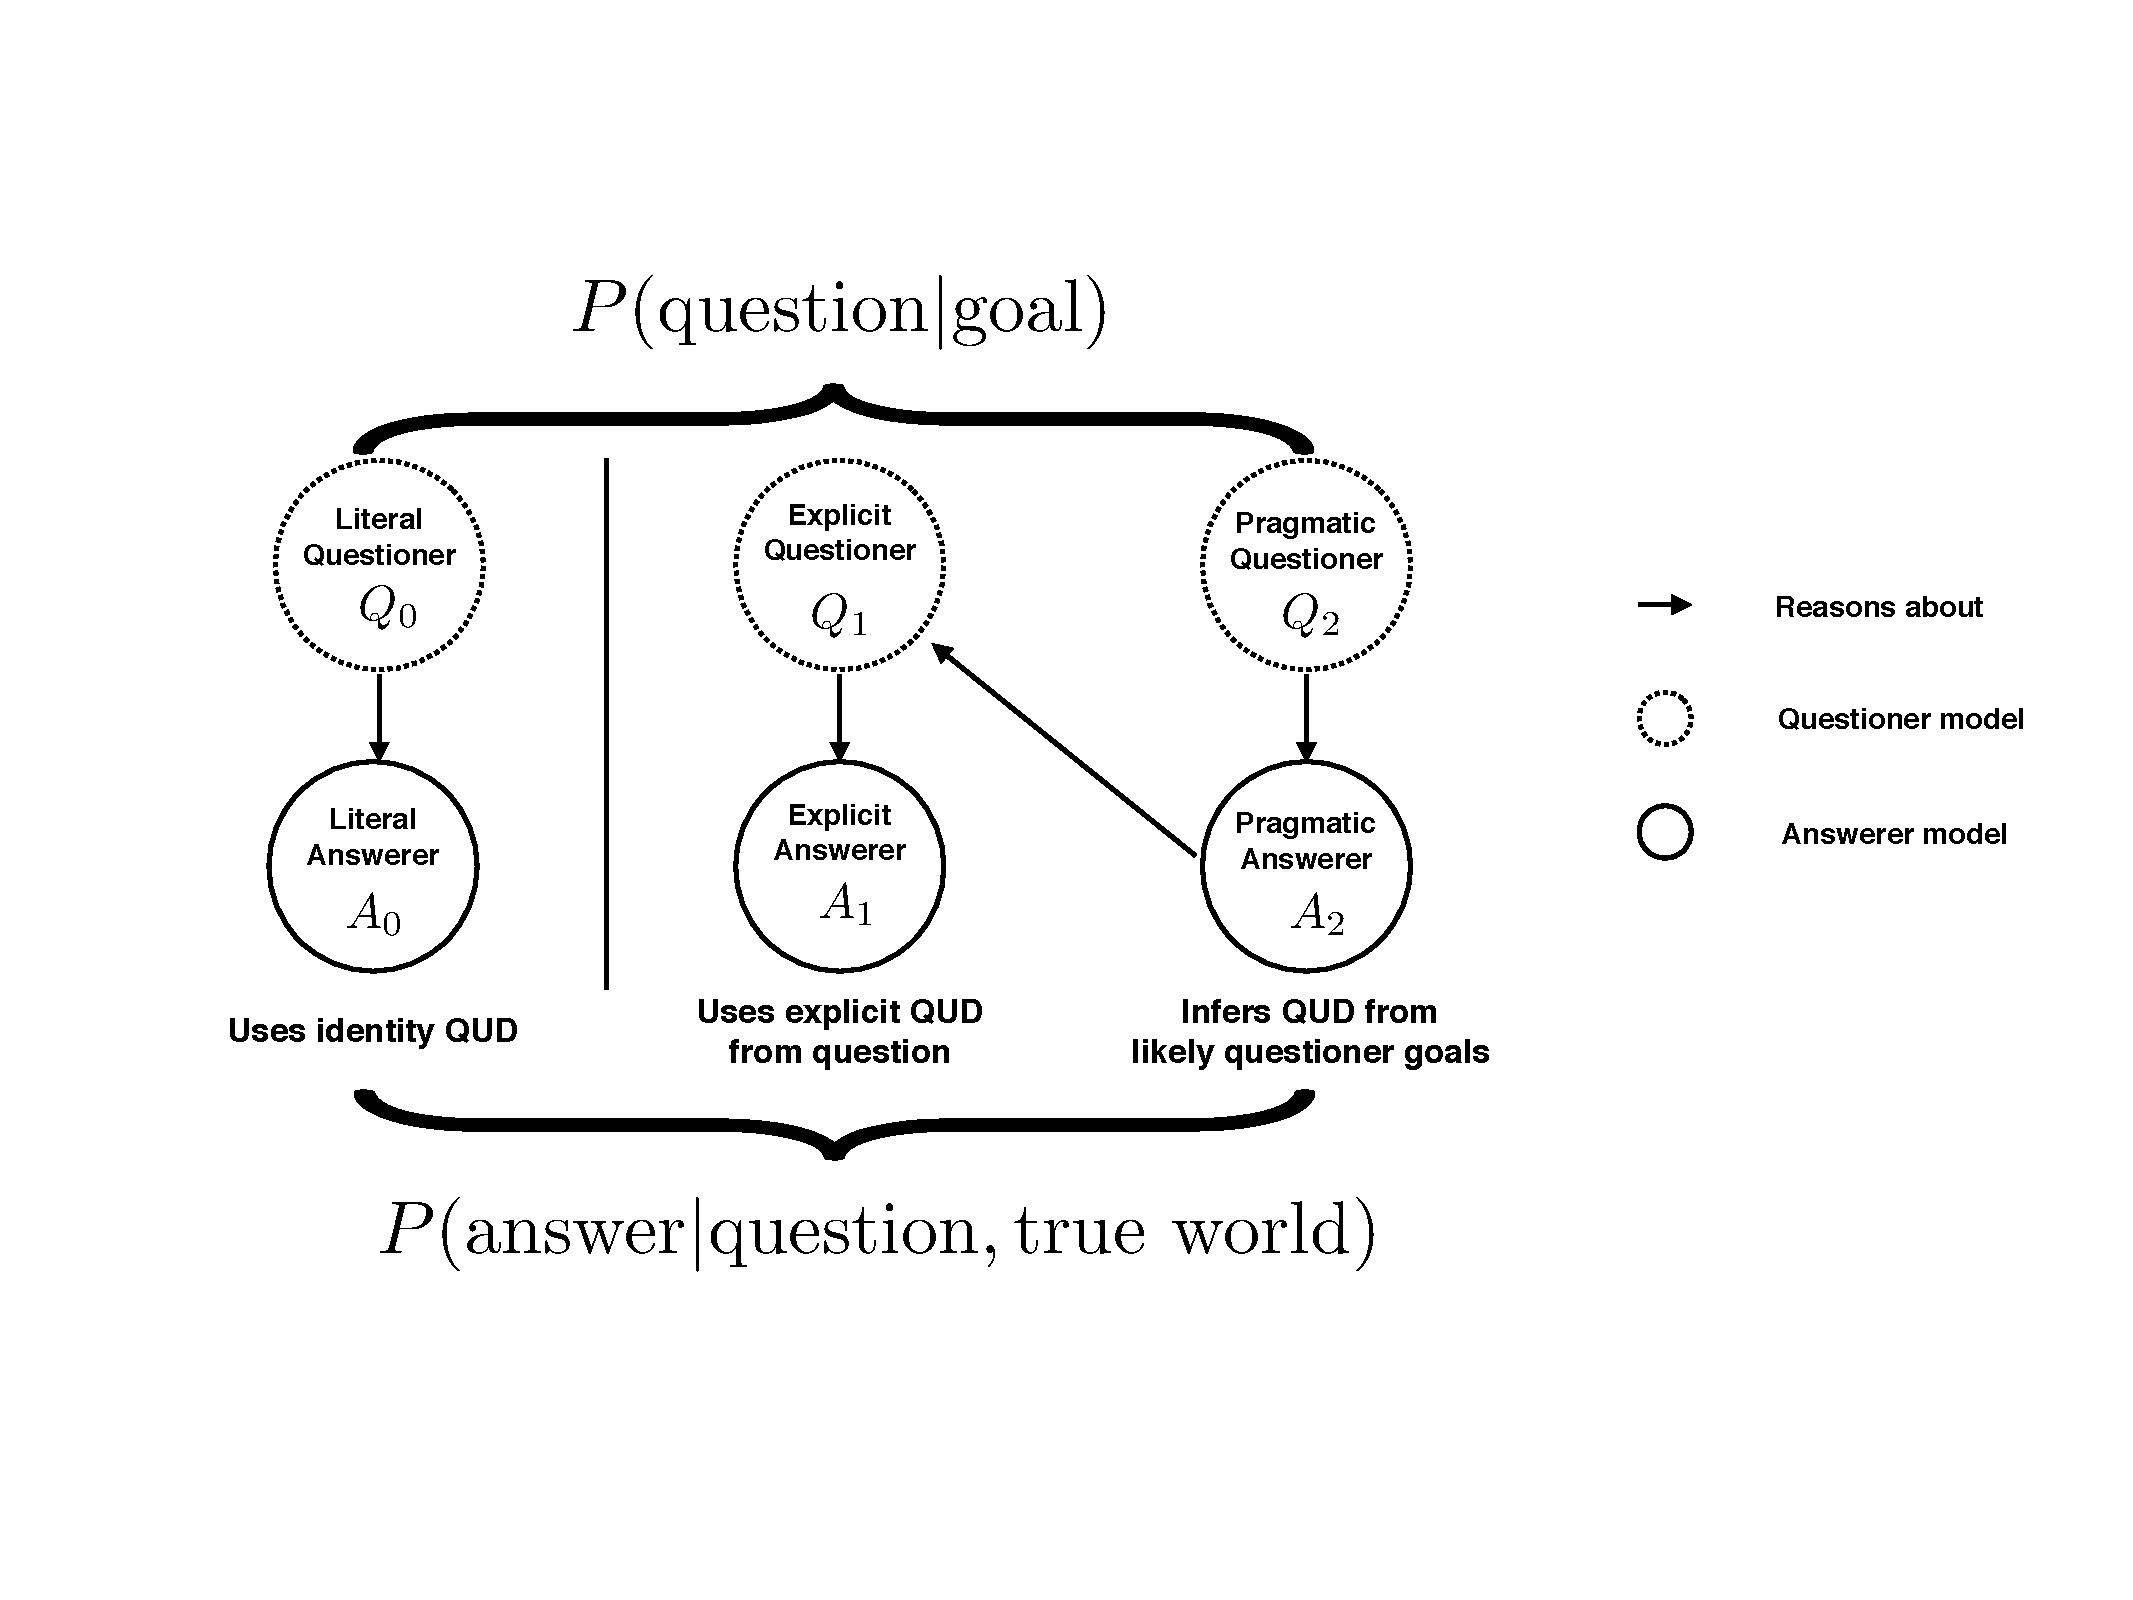
\includegraphics[scale = .5]{models.pdf}
\end{center}
\caption{Relationships between the questioner and answerer models we consider.}
\label{fig:models}
\end{figure*}

% HOW ARE THESE ADDRESSED IN RSA?
The listening problem and the speaking problem have been addressed separately in prior work within the Rational Speech Act (RSA) framework \cite{FrankGoodman12_PragmaticReasoningLanguageGames, GoodmanStuhlmuller13_KnowledgeImplicature, GoodmanFrank16_RSATiCS}, in which language understanding is formalized as recursive Bayesian inference. 
Pragmatic speaker agents choose utterances to minimize their partner's surprisal about the true state of the world -- a basic epistemic goal -- and pragmatic listener agents interpret utterances by inverting the speaker model. 
This basic framework has been used to account for a diverse selection of pragmatic phenomena including 
scalar implicature \cite{GoodmanStuhlmuller13_KnowledgeImplicature}, 
manner implicature \cite{BergenLevyGoodman16_LexicalUncertainty},
%prosody \cite{BergenGoodman15_StrategicUseOfNoise},
%the acquisition of word meanings \cite{FrankGoodman14_InferringWordMeanings}, and
generic language \cite{TesslerGoodman16_Generics}, and
interpretation of context-sensitive adjectives like ``tall'' or ``cheap'' \cite{LassiterGoodman15_AdjectivalVagueness}.

% HOW IS GOAL-RELEVANCE FORMALIZED IN RSA?
RSA models have also recently been extended to incorporate the critical notion of \emph{goal-relevance} into the speaker's utility \cite{Roberts96_InformationStructureDiscourse, WilsonSperber12_MeaningRelevance}. 
Instead of attempting to be maximally informative about the \emph{full} state of the world, a goal-relevant speaker ignores irrelevant dimensions and only attempts to be informative about relevant aspects. 
The projection function that collapses irrelevant dimensions is often called a Question Under Discussion (QUD) and is incorporated as a parameter of the speaker that a pragmatic listener may have uncertainty over and make inferences about.
RSA models with relevance have been used to capture non-literal language use like metaphor, irony, and hyperbole. 
In the case of hyperbole, for instance, a speaker who says ``It took a million years to get a table'' may be intending to be informative about the topic of their affective state (e.g. their frustration) rather than the exact time it took to get a table \cite{KaoWuBergenGoodman14_NonliteralNumberWords}.

% HOW IS OUR MODEL DIFFERENT FROM PAST MODELS (DIALOGUE!)
Although the social interplay between questioner and answerer may rely on that of the \emph{speaker} and \emph{listener} agents in previous RSA models, the minimal form of dialogue introduced by a question-answer exchange presents fundamentally new challenges.
Here, we build upon these recent modeling advances in several ways. 
First, while the role of a speaker in prior models is limited to production, and the role of listener is limited to interpretation, a question-answer exchange requires unifying the listening problem and speaking problem in a single agent. 
Addressing this problem in a rational model requires deriving the appropriate contingency between linguistic input and output.
Different kinds of input shift an agent's beliefs in different ways, motivating different kinds of responses. 

Second, the utilities used for previous RSA speakers cannot straightforwardly capture the utility of uttering a question, since questions don't provide direct information about the world to the listener.
While a declarative statement in our framework provides evidence about the true state of the world, as in previous models, we conjecture that a question is intended to be informative about the \emph{speaker's goals}. 
%Rather than defining the meaning of a question in terms of its possible answers, as in traditional linguistic theories, we treat it as a \emph{signal} that the listener can use to update their beliefs about the goals of the question-asker. 
When it is the listener's turn to speak, they can then generate statements that better address the goal-relevant aspects of the world. 
In the next section, we review the basic RSA framework and explore several different proposals for how agents interpret and respond to questions within this framework.

% HOW IS OUR MODEL DIFFERENT FROM PAST MODELS (QUESTIONS!)
%\footnote{That is, the literal meaning of a question does not seem to be new information about the world, per se. Questions do, of course, end up conveying information about the speaker's knowledge, needs, and so on---it is this conveyed information that we attempt to derive below.}. 

 %This diverges from previous RSA models in that the value of a question depends on information gained by the speaker (rather than listener), and that this information comes later in the (very short) conversation. 

%The account of questioner and answerer behavior we propose in this section is a an effort to synthesize linguistic theories of question semantics with rich, quantitative cognitive models of language understanding. 
%We jointly model the questioner's choice of question and the and answerer's choice of answer through recursive social reasoning, allowing the answerer to \emph{infer} the questioner's private goal from observing the context and question utterance. 

%If the questioner determines what question to ask by reasoning about likely answers, we must specify what kind of answerer they are reasoning about. We explore three increasingly sophisticated kinds of answerers, which serve as possible internal models used by the questioner, yielding three increasingly sophisticated kinds of questioners; these three models serve also independently as models of actual answerers. 
%The simplest agent, the literal answerer, simply attempts to be maximally informative about the true state of the world, ignoring the question;   
%the explicit answerer assumes that the question has a context-independent meaning and attempts to be informative with respect to that meaning (without inferring the questioner's underlying interests);  
%The latter model uses an extension of RSA to reason about the topic of conversation, as proposed by \citeA{KaoWuBergenGoodman14_NonliteralNumberWords}; it goes beyond previous work by using the explicit question as a (potentially indirect) cue to this topic. 

\label{sec:model}

\subsection{Preliminaries}

Our computational framework begins with the sets of world states, goals, and utterances (both questions and answers)\footnote{A particular choice of these sets specifies a model in the framework; they can be viewed as the basic cognitive primitives from which our framework derives question and answer behavior. Each experiment requires saying what these sets are for the scenario of interest.}. 
For concreteness, we use the scenario from \citeA{Clark79_IndirectSpeechActs} as an example throughout this section: 
\begin{description}
\item[$\mathcal{W}$:] a set of possible states of the world, such as the true price of a bottle of whiskey \{\$1, \$2, \dots, \$10\}. This may include arbitrarily many features of the world, such as the current weather, the location of nearby caf\'es, or the kinds of payment that the store accepts.
\item[$\mathcal{G}$:] a set of possible underlying questioner goals, such as learning the actual price of the whiskey or learning whether or not one can afford to buy the whiskey at all. 
Following previous RSA models, we formalize the key notion of a goal $g \in \mathcal{G}$ as a projection function $g: \mathcal{W} \rightarrow \widehat{\mathcal{W}}$ that maps a world state $w$ to a particular feature or set of features that the questioner cares about, which we denote $\widehat{w} = g(w)$. 
For example, when world states are prices, a customer's goal of learning the actual price of the whiskey is given by the identity function $g_{=}(w) = w$, while the goal of learning whether it is affordable is given by 
$$g_{<}(w) = \left\{\begin{array}{rcl}
1 & & w < 5 \\
0 & & \textrm{otherwise}
\end{array}\right.$$
such that all worlds where the agent can afford the whiskey are mapped onto one state, and all other worlds are mapped onto a different state.
\item[$\mathcal{Q}$:] a set of possible question utterances, such as ``Does a fifth of Jim Beam cost more than \$5?'' and alternatives like ``Do you accept credit cards?'' We take the literal meaning \den{$q$} of a question to be of the same type as a goal, such that a particular question utterance corresponds to a particular goal projection\footnote{This is equivalent to the partition semantics of \citeA{GroenendijkStokhof84_SemanticsOfQuestions}, as can be seen by considering the pre-image of such a projection: $q^{-1}(\hat{w})$.}. For example, the literal meaning of the question ``Does a fifth of Jim Beam cost more than \$5?'' is a function that maps all worlds $w$ such that $w > \$5$ to one value and all other worlds to a different value. Note that the correspondence between questions and goals is not necessarily symmetric: while every question corresponds to a goal, we do not expect that every possible goal corresponds to an easily articulated question utterance.
\item[$\mathcal{A}$:] a set of possible declarative utterances, such as ``It costs \$7.'' or ``Yes, it costs more than \$5.'' We take the literal meanings of these declarative utterances \den{$a$} to be truth-conditional: a map from world states to booleans. For instance, the utterance ``It costs \$7.'' would be true in the world where $w = \$7$ and false otherwise. 
\end{description}

Each of these sets is equipped with a prior, which we take to be shared in common ground.
This prior in principle allows us to explicitly model the knowledge that certain world states, goals, or utterances are \emph{a priori} more or less likely. 
Unless otherwise stated, we will assume uniform priors.
%and make the sources of any such knowledge explicit in the utility function. 
%Following previous RSA models, allowing questions and answers to have a production cost given by a function $C$; all else being equal, longer or less accessible utterances are less preferred.
These sets and their priors are the inputs we will vary to model different scenarios and experiments; the core computational machinery, described next, will be constant throughout the paper.
Our models of questioners depend on the answerer they imagine responses to come from, hence we first introduce a family of answerer models.

\subsection{$A_0$: Purely informative answerer}

We begin with the simplest possible answerer, $A_0$, which attempts to be informative about the state of the world without considering relevance to his partner's goals. 
Formally, $A_0$ hears a question utterance $q \in \mathcal{Q}$ and has private knowledge about the true world state $w \in \mathcal{W}$. 
He then uses a soft-max decision rule to choose an utterance $a \in \mathcal{A}$ proportional to the epistemic utility of that utterance to his communication partner: 
$$P_{A_0}(a | q, w) \propto \exp\{U_{A_0}(a;w)\}\cdot P(a)$$ 

\ndg{we don't need P(a) and P(q), since we have cost terms. is it worth including them for symmetry? i'd slightly favor leaving them out.}

We define the utility of the utterance using the information-theoretic measure of surprisal: the increase in an imagined interlocutor's $I$'s certainty about the true state of the world after hearing $a$. This surprisal is traded off against the cost $C(a)$ of producing the answer utterance:
\begin{equation}
\label{eq:A0utility}
U_{A_0}(a;w) =  \alpha_A \ln P_I(w|a) - \beta C(a)
\end{equation}
where $\alpha_A$ and $\beta$ are parameters weighting the importance of each term.

$A_0$ assumes that $I$ uses Bayesian inference to update their beliefs about worlds, conditioning on the literal meaning of the declarative utterance $a$ being true:
$$P_I(w|a) \propto \delta_{\textrm{\den{a}}(w)} P(w)$$
where $\delta_{e}$ is the delta function returning 1 when $e$ evaluates to true and 0 otherwise, and $P(w)$ is the (shared) prior over true states of the world. 
%In other words, the interpreter constrains the prior on worlds to the subset of its support that is consistent with the given utterance, and $A_0$ attempts to (soft)-maximize the probability of the true world in this posterior. 

This formulation of $A_0$ is equivalent to the pragmatic speaker $S_1$ for declarative utterances in previous RSA models \cite{GoodmanFrank16_RSATiCS}. 
It thus serves as a useful baseline, more charitable than a purely random speaker: if asked about a fifth of Jim Beam and knowing that it costs \$8, $A_0$ would prefer ``It costs \$8'' to ``It costs more than \$5'' or (falsely) ``It costs \$4'' simply because the former leads to an interpreter placing more probability on the true state of the world ($w = $ \$8).
Furthermore, because $A_0$ chooses utterances using the same core utilities as the more sophisticated models we consider, it serves as a ``lesioned'' speaker to evaluate the necessity of the relevance component. 


%%%
%\footnote{For the purposes of this paper, we assume answers are always full sentences, corresponding to truth-functional propositions that can be evaluated in a given world. The interpreter described is the simplest required to model such answers. For fragments such as `yes' or `Bob,' which can be used to answer questions like `Is dinner at 7pm?' or `Who got the promotion?' we would require a more sophisticated interpreter that can compositionally expand the fragment into a valid proposition, using the question. This is a standard operation in formal semantic models, and an interesting target for future research, but is not necessary for the experiments we report.}

\subsection{$A_1$: Relevantly Informative Answerer}

While $A_0$ is informative, he is not \emph{relevant}. When asked about the weather, he is just as likely to inform his partner about what he ate for breakfast as he is to say ``it's sunny.'' How do we incorporate relevance into the answerer's utility? 

Following \citeA{KaoWuBergenGoodman14_NonliteralNumberWords}, we formalize speaker relevance by means of a projection function. Instead of trying to increase the listener's certainty about the most fine-grained true world state, a relevant speaker only cares about the listener's certainty in a coarser space in which irrelevant features have been collapsed together. That coarser space is the image $\widehat{\mathcal{W}}$ of the goal-projection $g$. Crucially, a belief distribution over worlds, $P(w|\cdot)$, will project under $g$ to a belief distribution on this coarser space\footnote{For coarse goal-image spaces that are not discrete, it may be useful to replace the delta in this projection with a smoother kernel.}: 
$$\widehat{P^g}(\hat{w}|\cdot) = \sum_{w \in\mathcal{W}} \delta_{\hat{w} = g(w)} P(w|\cdot).$$
Thus, we may modify the utility from Eq. \ref{eq:A0utility} to define a relevantly informative answerer $A_1$: 
$$U_{A_1}(a; g, w) = \alpha_A \ln \widehat{P^g}(g(w)|a)  - \beta C(a).$$

%\begin{equation}
%U_{A_1}(a; g, w) = \alpha_A \ln \sum_{w' \in \mathcal{W}} K_g(w, w') P_I(w' | a) - \beta C(a)
%\end{equation}
%where $K_g(w,w')$ is a similarity function (or kernel) between worlds, determined by the goal. 
%For the discrete space of goals considered in the current work, we use the delta function $K_g(w,w') = \delta_{g(w)=g(w')}$ which combines the probabilities of all worlds that map to the same value in $\widehat{\mathcal{W}}$.\footnote{Note that $g$-projection is a generic operation on any probability distribution $P(w|\,\cdot)$, which we denote: 
%$$\widehat{P}^g(w|\, \cdot) = \E{P(w'|\, \cdot)}{K(w,w')}$$
%%\todo[inline]{rdh: not 100\% satisfied with this notation}
%}
\ndg{i switched back to using g-projection here, since we need it below. and the general kernel became a footnote, since we don't use it in this paper.}

%$$
%\begin{array}{rcl}
%U(a; g, w) & = & \ln \widehat{P^g_I}(g(w)|a) \\
%                 & = & \ln \sum_{w'\in\mathcal{W}} \delta_{g(w) = g(w')} P_I(w' | a) \\
%                 & = & \ln \sum_{w'\in\mathcal{W}} K_g(w,w')P_I(w' | a)
%\end{array}
%$$
In the context of a question answerer, the simplest assumption about the goal projection is that it is the literal meaning of the question:
%This modified utility suggests simply using the literal meaning of the question $q$ itself as the goal projection:
$$P_{A_1}(a|q,w) \propto \exp\{U_{A_1}(a; q,w)\} \cdot P(a)$$
This implements a literal answerer: $A_1$ directly interprets a question as an (epistemic) goal, then produces an informative utterance that reduces the questioner's uncertainty under that goal projection.
We note, however, that $A_1$ is not otherwise constrained in their set of possible answers by the question. 
For example, $A_1$ is capable of giving non-yes/no answers to polar questions to the extent that they resolve the literal goal raised by the question\footnote{Having the utility only depend on informativeness under the goal projection can lead to behavior where the goal-relevant answerer is happy to say something literally false as long as it maps to a truthful resolution of the coarser goal. Sometimes this is desired (as when we round the time to the nearest hour), but other times it is unintuitive. In principle, this problem could be solved by introducing the notion of a \emph{goal hierarchy} where the pure identity goal always has some small weight (see Exp.~2 for a formalization of this notion). In our simulations, however, we use a ``hard'' version of the same idea that removes literally false utterances from the possible answer set and then renormalizes the answer prior before computing the utility.}. 

$A_1$ may be sufficient for simple fact-based questions, like ``Who was the 16th president of the U.S.?'' given a rich enough semantic parser to supply the semantics of $q$ \cite{BerantChouFrostigLiang13_FreebaseQAPairs}. 
But the context-sensitivity and indirectness displayed in everyday communication suggests that deeper social reasoning may be at play. 
To explore more sophisticated answerers that reason about context and their partner's underlying goals, we must first address the problem of how a speaker chooses between questions.

\subsection{$Q_i$: Questioners}

If the utility of uttering a declarative statement is imparting information about the true state of the world, what is the utility of uttering a question? We begin by assuming that a questioner aims to \emph{learn information relevant to a private goal}.
%
In order to choose a question that results in useful information, the questioner reasons about how her dialogue partner would respond in different possible states of the world. 
She then selects among questions proportional to the extent that the answers they would elicit reduce her own uncertainty about goal-relevant information.
%

% This is a divergence from previous RSA models, where agents choose utterances with the goal of imparting information about the state of the world.

More formally, a questioner agent takes a goal $g \in \mathcal{G}$ as input and returns a distribution over question utterances $q \in \mathcal{Q}$ by solving a simple planning problem involving two components: (1) which answers are likely to come back after asking this question, and (2) how much would be learned from each of those answers. Critically, in order to solve either of these parts, the questioner must have in mind an imagined answerer who hears her question and responds appropriately: thus, we have a family of questioners $Q_i$, each using the corresponding answerer $A_i$:
%
$$
\begin{array}{lcl}
P_{Q_i}(q|g)  & \propto & \exp\{U_{Q_i}(q;g)\} \cdot P(q)\\
U_{Q_i}(q;g) & = & \alpha_Q \E{P(w)}{ \E{P_{A_i}(a|q,w)}{IG^g(a,q)}}\\
%	 & = & \alpha_Q \sum_{w\in\mathcal{W}} P_{A_i}(a|q,w)P(w) IG^g(a,q) 
\end{array}
$$
%
The expectation describes a questioner who first imagines what state the answerer might know the world to be in, then imagines what answer the answerer would thusly provide.
The value of this answer depends on its \emph{information gain} $IG^g(a,q)$: the gap between the questioner's beliefs about the $g$-relevant state of the world before and after hearing an answer.\footnote{A cost term $C(q)$ would also be appropriate in this utility, but for the cases we consider in this paper, the questions of interest have the same length, so we omit cost for simplicity.} Drawing again upon information theory, we formalize the notion of information gain using the Kullback-Leibler divergence between the $g$-projected world prior and posterior after hearing $a$:
%
$$
IG^g(a,q) = \KL{\widehat{P^g}(w|q, a)}{\widehat{P^g}(w)}\\
$$
%
In order to anticipate her posterior beliefs after hearing an answer, the questioner must again make use of an imagined answerer, but now imagining herself as a listener in the future and inverting that model to infer the true world the answerer was trying to communicate:
$$P(w|q,a) \propto P_{A_i}(a| q, w)P(w).$$

The above equations specify a questioner for each answerer model. $Q_0$, who plans their question by reasoning about the likely responses of $A_0$, does not prefer any utterance over any other, because they will all lead to the same distribution of (informative but not necessarily relevant) answers. $Q_1$, on the other hand, expects $A_1$ to directly interpret her question as a goal and respond informatively and relevantly, thus allowing for some questions to be better than others. It therefore instantiates a version of the expected information gain measure of usefulness proposed by Optimal Experiment Design (OED) models \cite{coenen2018asking}. Critically, in contrast to classical views \cite<e.g.>{GroenendijkStokhof84_SemanticsOfQuestions} the questioner's behavior is not necessarily governed fully by the semantics of the question she asks, but by what she actually expects her partner to say after hearing it. They coincide when reasoning about the simple $A_1$ answerer, but we next turn to a more socially perspicacious answerer where they diverge.

\subsection{$A_2$: Goal-Sensitive Answerer}

%\begin{table*}[h!]
%\centering
%\begin{tabular}{ p{5.15cm} | p{4cm} | p{7cm}}
%Case study &	Cue to goals	& Model variations \\
%\hline
%Clark (1979); Exp 4 &	prior verbal context	& likely goals depend on context \\
%\hline
%Groenendijk \& Stokhof (1984) & non-verbal features & multi-dimensional world representation, expanded space of answers \\
%\hline
%Gibbs Jr. \& Bryant (2008)  &	current world state &	expanded space of possible goals\\
%\hline
%Clark (1979); Exp 5 & choice of question & expanded space of question alternatives 
%\end{tabular}
%\\[1.5pt]
%\caption{Overview of the key features of the case studies we consider, and the modeling choices we make in each case. Note that while representations of sets $\mathcal{W}, \mathcal{Q}, \mathcal{A},$ and $\mathcal{G}$ adjust to capture the details of each scenario, the overall model framework is held constant.} 
%\end{table*}

Now that we have defined the utility of asking a question, we can construct our final pragmatic answerer: $A_2$. The speaker component of this answerer attempts to informatively and relevantly address the questioner's goal, like $A_1$. The listener component, however, accounts for the generative process of an asker with an underlying goal rather than taking that goal to be identical to the literal meaning of the question. That is, $A_2$ assumes that the question was produced by a rational agent $Q_1$, who is trying to address a private goal $g \in \mathcal{G}$, and then attempts to be relevantly informative with respect to his posterior over \emph{underlying} goals given the question $P(g|q)$:
\begin{equation}
U_{A_2}(a; q, w) = \alpha_A \E{P(g|q)}{\ln \widehat{P^g_I}(w|\,a) }- \beta C(a)
% \alpha_A \sum_{g \in \mathcal{G}} P(g|q) \ln \widehat{P^g_I}(w|\,a) - \beta C(a)
\end{equation}
%The \textbf{pragmatic answerer} also evaluates answers with respect to how well they address the questioner's goal, but doesn't take the question's explicit meaning at face value. Instead, the pragmatic answerer reasons about which underlying goals $g$ are likely given that a question $q$ was asked, and chooses answers that have high expected informativity:
%
Reasoning backwards from questions to goals is a simple Bayesian inversion of $Q_1$ using the prior on goals:
$$
P(g|q) \propto P_{Q_1}(q|g)\cdot P(g)
$$

Here we have defined $A_2$ recursively in terms of $Q_1$. This recursion could give rise to an arbitrarily deep chain of nested reasoning where $A_{i}$ infers a posterior over underlying goals by inverting $Q_{i-1}$, and so on, terminating in the base case $A_1$, which uses the literal question semantics. In this paper, we consider models up to a depth of $i=2$; beyond this depth there are no qualitative changes in the model's behavior for the cases we examine\footnote{Recent systematic model exploration by \citeA{frank2017rational} suggests that recursive depth trades off with the soft-max optimality parameter $\alpha$. Because these two parameters are not generally identifiable, we fix the maximal level of recursion and achieve the behavior of higher levels of recursion by allowing $\alpha$ to vary.}. 

The framework specified above has three free parameters: separate $\alpha$ parameters for the questioner and answerer, and an answerer cost weight $\beta$.
(In principle, this parameterization could be loosened by allowing different parameters at different levels of recursion, or tightened by requiring the questioner and answerer to use the same $\alpha$.)
%$A_2$ and $Q_2$ can be interpreted as pragmatic agents who are capable of going beyond    and $Q_2$, which can be interpreted as an agent who rationally selects a question not simply for its literal meaning but for the signal it provides about her underlying beliefs. 
This concludes our specification of the model space, giving a set of three answerers and three corresponding questioners (see Fig. \ref{fig:models}). In the remainder we consider evidence that allow us to select among these models.\footnote{We have implemented these models in WebPPL, a probabilistic programming language \cite{GoodmanStuhlmuller14_DIPPL}. Reproducible experimental materials as well as code for all reported analyses and model simulations is available at \url{https://github.com/hawkrobe/Q\_and\_A}}
 

%For all of the questioner and answerer models, we can vary how strongly optimizing they are---that is, to what extent they are sampling from the distributions defined above, and to what extent they deterministically choose the most likely element. For any such distribution over utterances, we introduce an optimality parameter $\alpha$ and transform it by $ P'(x) \propto P(x)^{\alpha} $. Furthermore, we have set the answer prior in all answerer models such that outright false responses are excluded. The answerer models naturally assign very low, but non-zero probability to these options (because they are minimally informative). However, we set them to zero probability for the sake of simplicity in reporting and visualizing predictions.
%



\section{Case studies in answerer sensitivity}

In this section, we illustrate our \emph{answerer} models through several classic goal-sensitivity effects reported by \citeA{Clark79_IndirectSpeechActs}.\footnote{These examples are implemented and runnable at \url{forestdb.org/models/questions-answers.html}} These case studies center around three empirical observations about the factors determining answerer behavior in dialogue. First, and most obviously, answers should be sensitive to the surface form of the question utterance: ``What time do you close tonight?'' should elicit a different distribution of responses than ``What is the price of a fifth of Jim Beam?''. Second, answers should be sensitive to context: the \emph{same} question utterance elicits different responses across contexts where different goals are more or less likely. Third, and most subtly, answers should be sensitive to the cue provided by the question utterance itself toward the questioner's underlying goals.


% We proceed to demonstrate the way our model addresses four classic examples of question and answer pragmatics from the psycholinguistics literature. There has been little use of questioner behavior as a dependent variable in previous literature, hence our examples explore the sensitivity of the answerer to plausible goals of the questioner. 
%These examples do not serve as a strong test of our model's predictions, because we will have to make post-hoc assumptions about prior distributions or goal spaces in each study.

%Yet it is important to show that our framework can accommodate these results.
%We see two additional benefits to re-formulating explanations from the original studies within our modeling framework: (1) the case studies are instructive as examples of how different components of the model interact to generate results and (2) by placing all four studies in a common framework, we more clearly see their commonalities and differences. 

%\ndg{i feel like this section gets pretty quickly lost in the weeds.... maybe we can reorganize it around the effects or model components explored? and move some of the details and conceptually redundant pieces to appendices?}

% \begin{figure*}[t!]
%\begin{center}
%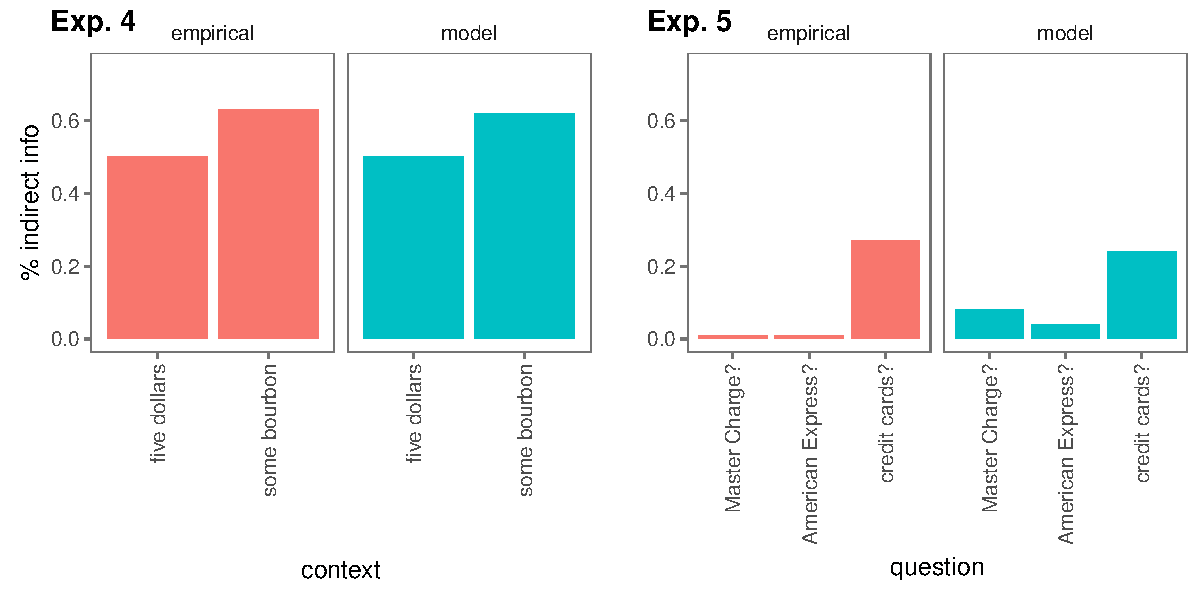
\includegraphics[scale = .6]{clarkCaseStudies.pdf}
%\end{center}
%\vspace{-.25cm}
%\caption{Comparison of questioner goal posteriors that the pragmatic answerer model infers after hearing two different question utterances in Clark (1979), Experiment 5.}
%\label{fig:clarkResults}
%\end{figure*}

%\begin{table*}[t]
%\centering
%\begin{tabular}{ p{3cm} | r | r ||||||  r | r }
%& \multicolumn{2}{c||||||}{Empirical} & \multicolumn{2}{c}{Model} \\
%\hline
%&           \% literal &   \%  info &           \% literal &   \%  info    \\
%\hline
%``Some bourbon'' &   0.37 & 0.63 &  0.38 & 0.62 \\
%\hline
%``Five dollars''     & 0.50 & 0.50 & 0.50 & 0.50 \\
%\specialrule{2.5pt}{1pt}{1pt}
%``Master Charge cards?'' &   1.00 & 0.00 &  0.92 & 0.08 \\
%\hline
%``American Express cards?''     & 1.00 & 0.00 & 0.96 & 0.04 \\
%\hline
%``Credit cards?''     & 0.73 & 0.27 & 0.76 & 0.24 \\
%\end{tabular}
%\\[1.5pt]
%\caption{Comparison of model predictions and data from Clark (1979). Shows the proportion of responses to the question ``Does a fifth of Jim Beam cost more than \$5?'' when paired with two contexts: ``I want to buy some bourbon'' (``Some bourbon'') and ``I've got \$5 to spend'' (``Five dollars''). } 
%\label{table:clark79exp4}
%\end{table*}

\subsection{Sensitivity to question utterance}

The minimal requirement for any answerer model is that it behaves differently in response to different questions. This can also be considered a special case of the minimal requirement for a dialogue agent: that their behavior at time $t$ is in some way dependent on their partner's at $t-1$. %We briefly illustrate this phenomenon in our model using two example sentences lightly adapted from \citeA{Clark79_IndirectSpeechActs}.
Consider the problem faced by a liquor store cashier answering one of the phone calls reported by \citeA{Clark79_IndirectSpeechActs}: they may be asked one of two questions: $q_t$ (``What time do you close tonight?'') and $q_p$ (``What is the price of a fifth of Jim Beam?''). How do our answerer models respond to each of these questions?

To model this situation, we take a world $w \in \mathcal{W}$ to be a tuple containing the closing time and the price of Jim Beam at the store in question. Thus, $\mathcal{W}$ is the set of all possible tuples $w = (t, p)$, where $t$ is a time in the (simplified) set $\{9\textrm{pm},10\textrm{pm}\}$ and $p$ is a price in $\{\$4, \$5, \$6\}$. Similarly, we consider a simplified set of answers $\mathcal{A}$: an answerer may either state a time $a_{t_i}$ (``We close at 9:00.'') or the price of Jim Beam $a_{p_i}$  (``A fifth costs \$5.''). These utterances evaluate to true in a particular world $w$ if and only the stated dimension has the stated level.

Our informative answerer $A_0$ does \emph{not} reply differently to the two questions. In either case, he slightly prefers to inform the questioner about the price using $a_{p_i}$ because he reasons that a literal interpreter $I$, after hearing such an utterance, would be left with uncertainty over only two possible worlds (where the closing time is either 9:00 or 10:00) rather than the three possible worlds consistent with an utterance stating the true time (where the price is either \$4, \$5, or \$6).

Both $A_1$ and $A_2$, on the other hand, appropriately give different answers to the two questions, though for different reasons. $A_1$ gives different answers because the two questions simply have different literal meanings: $q_t$ projects a world $w_i = (t_i, p_i)$ to its first element, $q_t(w_i) = t_i$, whereas $q_p$ projects $w_i$ to its second element $p_i$. In this example, because we take the space of goals $\mathcal{G}$ to contain these same two projections, $A_2$ makes essentially the same inference. He reasons it's more likely, via Bayes' Rule, that a questioner agent $Q_1$ who chose to ask $q_t$ would have the goal of learning the closing time than the price, and updates his beliefs accordingly.

These answerers then choose an utterance that \emph{relevantly} addresses the goal they inferred. $a_{p_i}$, for instance, would leave the questioner with perfect information about $p_i$ but gives no information at all about $t_i$. Thus, it would be a preferred response to $q_p$ and a dispreferred response to $q_t$. This shows the desired sensitivity to question.

\subsection{Sensitivity to context}

Next, we show how our models can provide different---sometimes over- or under-informative---answers to the same explicit question, depending on context. For this illustration, we consider the results of Experiment 4 from \citeA{Clark79_IndirectSpeechActs}. Recall that liquor merchants were more likely to give over-informative answers (specifying exact price) to the question ``Does a fifth of Jim Beam cost more than \$5?'' in the uninformative context (``I want to buy some bourbon'') than in the five dollar context (``I've got \$5 to spend''). Which of our answerer models, if any, shows a similar sensitivity to context?

Our space of possible worlds consists of possible prices for the whiskey: $\mathcal{W} = \{\$1, \dots, \$10\}$. We consider two possible goals with equal prior probability: $g_=$, learning the actual price of whiskey,  and $g_>$, learning whether or not the agent can afford to buy the whiskey at all (i.e. whether the price is greater or less than the amount the agent has in their pocket). The set of answers $\mathcal{A}$ includes exact prices $a~\in~\{\$1, \dots, \$10\}$ as well as ``yes'' and ``no.'' 
Although it does not change the qualitative effects of interest, we assume that bare ``yes/no'' answers are slightly less costly to produce than more informative ``price'' answers.

%Because the question was fixed in the experiment, the question space $\mathcal{Q}$ simply consists of the single question $q = $``Does a fifth of Jim Beam cost more than \$5?''\footnote{Note that because there are no alternatives for the ``pragmatic answerer'' to consider, they are not strictly engaging in Gricean reasoning; obvious alternatives like ``How much does Jim Beam cost?'' do not significantly change the model behavior in this case, but we omit them to isolate the effect of the QUD prior in this example.}  

We model the context sentence as a statement which the answerer must interpret before interpreting the question; we assume that it has the effect of shifting the answerer's beliefs about likely questioner goals $P(g)$. When the context is ``I'd like to buy some whiskey,'' we assume no shift from the goal prior: $P(g_= | c) = P(g_> | c) = 0.5$. When it is ``I only have \$5 to spend,'' we assume a shift toward the comparison goal: $P(g_> | c)~=~.99$.\footnote{This can be seen as a case of ``inquisitive content'' in a declarative sentence \cite{ciardelli2018inquisitive}: the sentence is literally informative about how much money the speaker has but it has the same inquisitive effect of shifting the listener's expectations about the speaker's goals as a question does. This could be derived via further pragmatic inference or via an explicitly inquisitive semantics. While our framework is compatible with either approach (see General Discussion), this is the only example of such a ``hybrid'' declarative utterance that arises in the paper, so to avoid complicating our presentation, we stipulate the effect and leave the formal derivation for future work.}

Now, $A_0$ is unable to show sensitivity to context for the same reason that he did not show sensitivity to the question utterance in our first simulation: he does not adjust his beliefs on the basis of what he hears. Thus, he always prefers to say the exact price (e.g. ``The whiskey costs \$6'') because it leaves less uncertainty about the true state of the world.

Because $A_1$ uses the literal meaning of the question, which is context-independent and not tied to the questioner's goals, he does \emph{not} give different responses in the two contexts. 
In either case, he addresses the goal of finding out whether the price is more than \$5, so his answer distribution is only determined by the relative costs of giving a yes/no answer and an exact answer: they provide equivalent information about whether the true price is greater than or less than \$5. 

Finally, $A_2$ is context-dependent in the same way as \citeA{Clark79_IndirectSpeechActs} observed. 
When the question is prefaced with ``I only have \$5 to spend,'' which shifts the answerer's beliefs about goals strongly toward $g_>$ (equivalent to the literal meaning of the question), then $A_2$ behaves like $A_1$. 
However, when the question is prefaced with ``I'd like to buy some whiskey,'' which leaves in place the answerer's uniform prior over goals, then the \emph{exact price} answer is favored more strongly. This answer is much more informative in the case when the questioner's goal is to know the exact price, and no worse in the other case. The expected value of the non-literal answer is thus higher, and the answerer responds proportionally. 

This example demonstrates that decoupling the inferred goal from the explicit meaning of the question is necessary to provide the model freedom to reflect context, though the exact shift in goals depending on context is assumed rather than derived. 

%The output of $A_2$ is shown in Fig. \ref{fig:clarkResults}, compared with empirical results from \citeA{Clark79_IndirectSpeechActs}\footnote{The responses in \citeA{Clark79_IndirectSpeechActs} were tallied in three categories: literal answer only $(n_l)$, information only $(n_i)$, or both literal answer \emph{and} information $(n_b)$. For the purposes of this case study, we are only interested in the ratio of literal answers to information answers: $p_l = n_l/(n_l+n_i)$ and $p_i = n_i/(n_l+n_i)$.}  
% This asymmetry arises in our model due to the fact that an exact price is much more highly informative than a literal response with respect to the ``exact price'' goal $g_=$, and if there is uncertainty over which goal is in fact the case, it is worth erring on the side of over-informativeness. This matches the empirical trend, which also favored the exact price answer (at probability $0.57$) over the literal answer (at probability $0.41$).

%This arises because both responses are equally informative with respect to learning whether or not the agent can afford the whiskey, $g_>$, so the response likelihoods fall back to the answer prior. This also matches the empirical trend, where the exact price and literal answer were equally likely.

%Note that the literal and explicit answerers do not take into account the questioner's underlying goals and therefore cannot reason about the way contextual factors may be informative about these goals. Hence, they do not make different predictions in the two contexts. The literal model predicts that the answerer is equally likely to say the true Boolean answer and the true numerical answer, and the explicit model predicts that the answerer will always give the true Boolean answer, since it is the explicit question being asked. This suggests that our pragmatic \emph{answerer} is consistent with human behavior in psychologically interesting situations, passing a first, qualitative, test. 

%\begin{table*}[t!]
%\centering
%\begin{tabular}{ p{5cm} | r | r ||||||  r | r }
%& \multicolumn{2}{c||||||}{Empirical} & \multicolumn{2}{c}{Model} \\
%\hline
%&           \% literal &   \%  info &           \% literal &   \%  info    \\
%\hline
%\end{tabular}
%\\[1.5pt]
%\caption{Comparison of model predictions and data from Clark (1979), Experiment 5. Shows the proportion of literal and over-informative responses restauranteurs gave to each of three different questions from a customer inquiring about credit cards.} 
%\label{table:clark79exp5}
%\end{table*}

\begin{figure*}[t]
\begin{center}
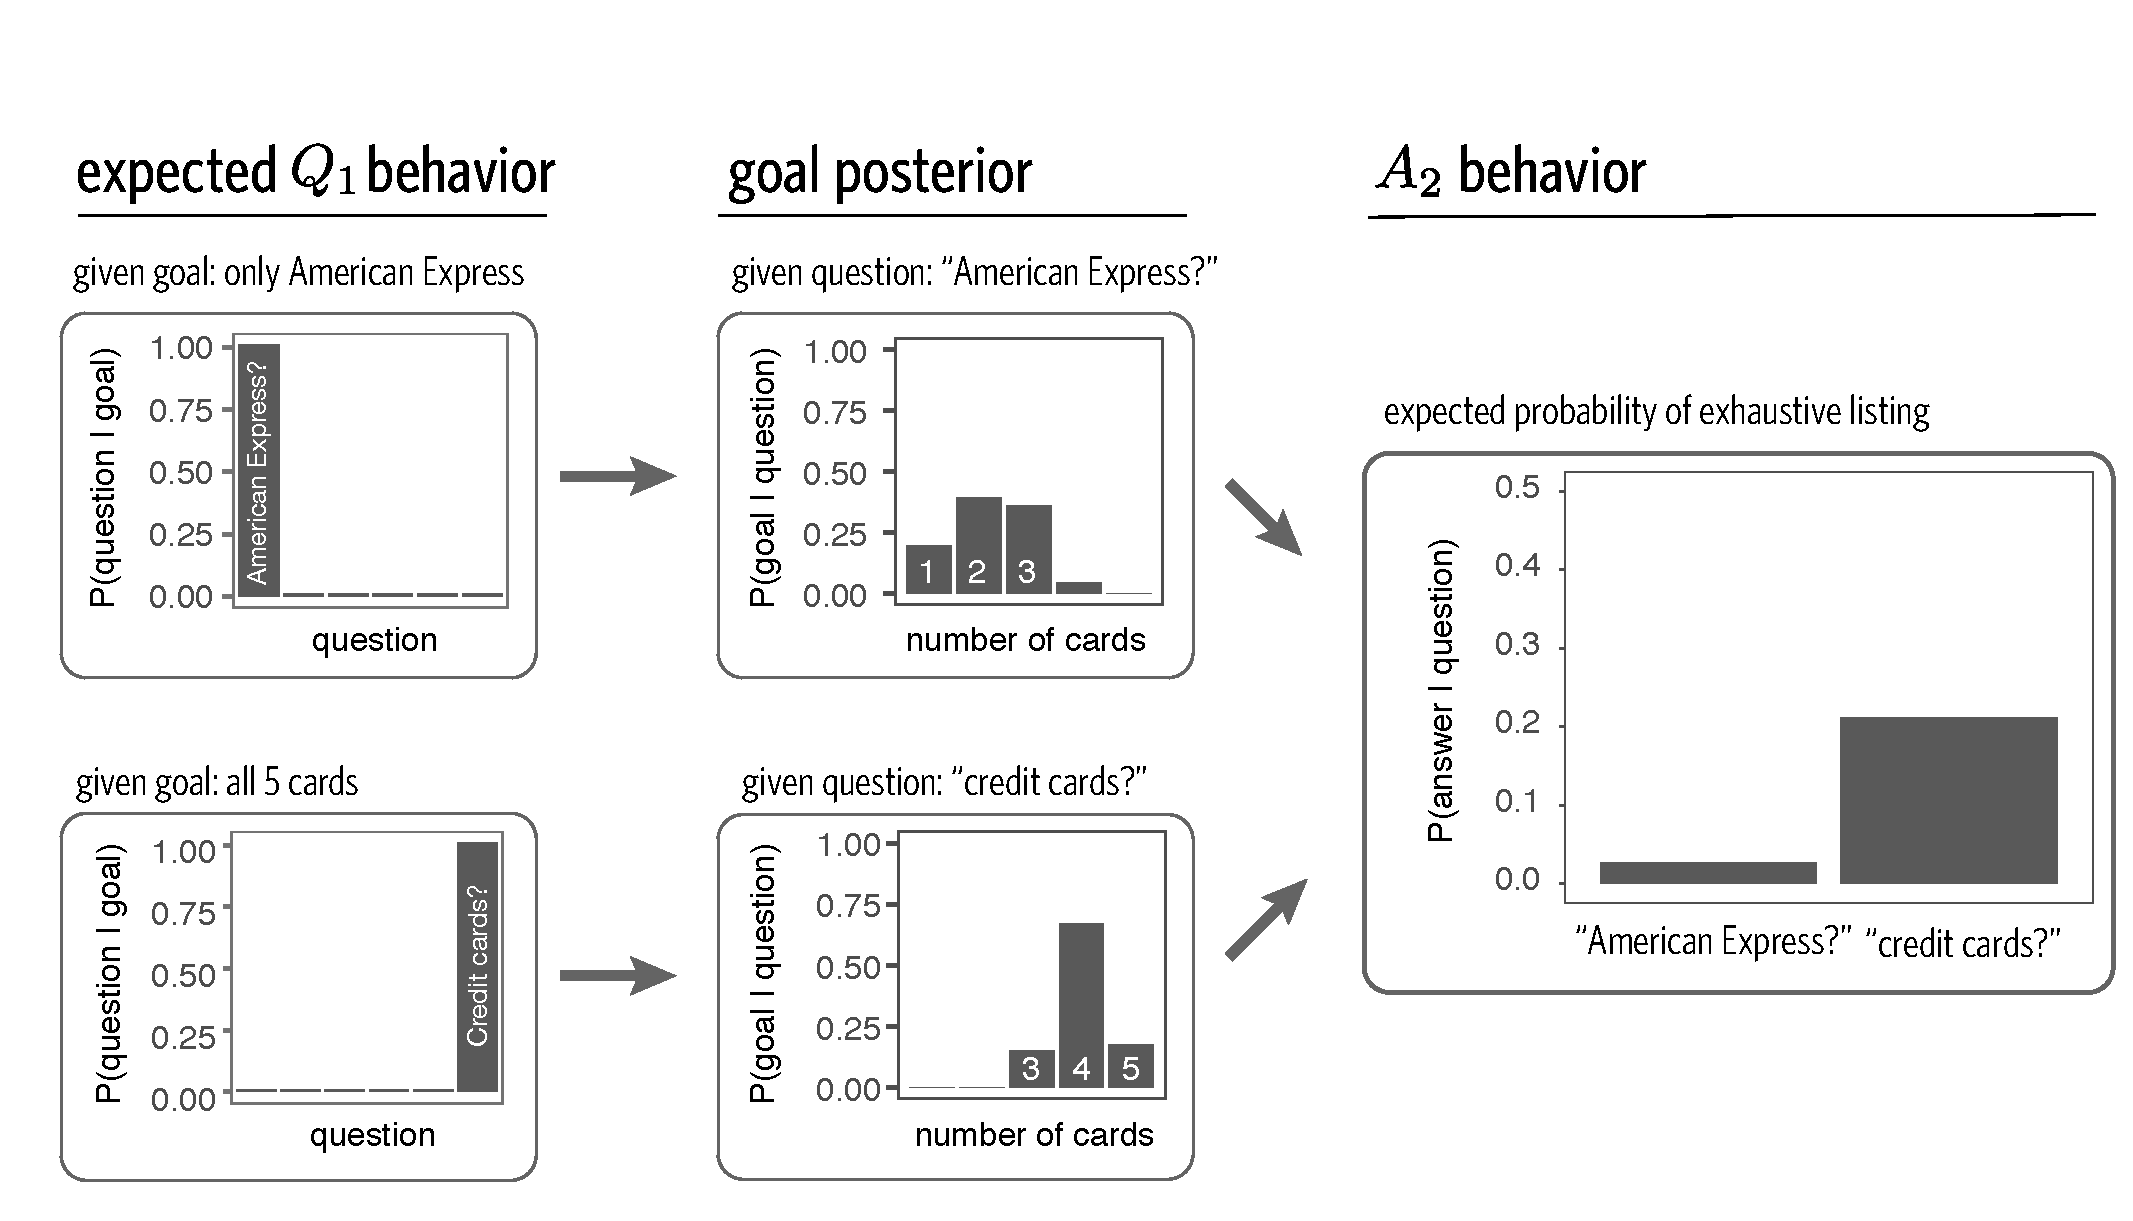
\includegraphics[scale=.5]{simulations/clarkExampleFig}
\end{center}
%\vspace{-1cm}
\caption{Illustration of how $A_2$ uses the questioner's utterance as a cue to their underlying goal and responds relevantly, thus producing the sensitivity reported by Clark (1979). We set the optimality parameter $\alpha_A = \alpha_Q = 50$ and cost $\beta = 5$. The middle column is the marginalized goal posterior showing the expected number of cards; right column is expected probability of exhaustive listing (vs. literal yes/no answer) marginalized over all possible worlds.}
\label{fig:clarkExample}
\end{figure*}

\subsection{Sensitivity to relationship between goal and question utterance}

% Our final scenario demonstrates the role of the questioner component in our pragmatic answerer model. Because the question space in the previous computational experiments only contained one element for simplicity, the pragmatic answerers' inferences were entirely based on the context and the QUD prior. One of the most interesting and novel predictions of the RSA model, however, is that the questioner's choice of utterance itself should guide a pragmatic answerer's inferences about likely underlying goals. The choice to ask one question instead of another provides information about the questioner's goal. While there are few previous experimental results using questioner behavior as the \emph{dependent variable}, there is some work manipulating the question asked as an \emph{independent variable} and testing how it affects answers.

The subtlest effects of answerer sensitivity go beyond the overt question utterance and context alone; given the same context, answerers may respond to one question according to its literal meaning but another using more indirect or overinformative statements. One of the key predictions of  $A_2$ is that these effects are due to different inferences about the questioner's \emph{underlying goals} on the basis of the questioner's choice of utterance itself. 

For our final case study, we consider Experiment 5 from \citeA{Clark79_IndirectSpeechActs}, which called restaurants and asked one of four yes/no questions about which \emph{credit cards} the restaurant accepted. We focus on three\footnote{
The fourth question was ``Do you accept any kinds of credit cards?'' We view Clark's results for this question as an example of M-implicature: by using a more costly utterance with the same literal meaning as question (3), the meaning becomes marked. Rational speech act models capture M-implicature by introducing \emph{lexical uncertainty} \cite{BergenGoodmanLevy12_Alternatives}, where both speaker and listener begin their inference with uncertainty over the literal meaning of utterances. % By jointly reasoning about an utterance's meaning and the world state the speaker is trying to convey, more costly utterances are mapped to meanings with lower prior probability, allowing a pragmatic inference that ``Do you accept any kinds of credit cards?'' most likely means something like ``What kinds of credit card do you accept?'' 
Because this is the only example of M-implicature that arises in this paper, and this is not the critical result from the experiment, we exclude it from our discussion.%believe that a presentation of the full lexical uncertainty model would be unnecessary and confusing to the reader.
}:
%%%
\begin{enumerate}
\item ``Do you accept MasterCard?'' 
\item ``Do you accept American Express?''
\item ``Do you accept credit cards?'' 
\end{enumerate}
%He analyzed the likelihood that the respondent gave a literal yes/no answer, compared to the likelihood of giving the exhaustive list of exactly which cards were accepted.  
\citeA{Clark79_IndirectSpeechActs} found that (1) and (2) were nearly always answered literally, with a `yes' or `no', while (3) was significantly more likely to be answered with full information (a list of al credit cards accepted). Which, if any, of our answerer models show this pattern of responses? % (see Table \ref{table:clark79exp5}). 
%As in the first case study above, we are only interested in the ratio of literal answers vs. over-informative answers $p_l = n_l/(n_l + n_i)$ and $p_i = n_i/(n_l + n_i)$, not in responses including both. 

We formalize the scenario as follows. The set of possible worlds $\mathcal{W}$ is given by the power set $\mathcal{P}(\mathcal{C})$, where $\mathcal{C} = \{$Visa, MasterCard, American Express, Diner's Club, and Carte Blanche$\}$, the set of five possible credit cards. %This power set contains all $2^5 = 32$ subsets of cards that the restaurant might accept. 
The prior distribution over worlds, $P(w)$, can in principle take into account the empirical likelihoods of restaurants accepting different cards, but we treat them as uniform to make the dynamics of our simulations clearer. % Clark reports these likelihoods to be 72, 71, 38, 12, and 10\% for Visa, Master Card, American Express, Diner's Club, and Carte Blanche, respectively. 

The question space $\mathcal{Q}$ contains the five basic questions (``Do you accept $c$?" with $c \in \mathcal{C}$ one of the five cards) in addition to ``Do you accept credit cards?'' For the literal semantics of the five basic questions, indexed by $c$, we use the function $q_c(w) = \delta_{c \in w}$, which projects worlds to a boolean corresponding to whether they accept card $c$ or not.
%partitions the space of possible worlds into two cells: one  in which card $c$ is accepted and another in which it is not accepted. 
The latter question $q_{any}(w)  = \delta_{|w| > 0}$ projects to a boolean corresponding to whether any cards are accepted at all. %The prior distribution $P(q)$ over these questions is proportional to question length, which happens to be uniform.

The answer space $\mathcal{A}$ includes lists of cards (e.g. ``the cards we accept are Visa and MasterCard''), which are interpreted exhaustively, and  `yes' and `no.' We take the denotations of these polar responses to depend on the literal meaning of the previous question: $a_{\text{yes}}(w;q) = \delta_{\textrm{\den{q}}(w)}$ and $a_{\text{no}}(w;q) = \delta_{\neg \textrm{\den{q}}(w)}$.
\ndg{the delta functions are a little sloppy: since they take a boolean but return a 0/1, here the typing is wrong. we can ignore this, or just get rid of the deltas since it's fine if all semantics is in booleans, not real.}
 %Thus, the restauranteur could respond to the question ``Do you accept Master Charge cards?" by saying ``Yes'' or by saying something like ``We accept Visa and Diner's Club." 
%As in our early case study of Clark's (1979) whiskey experiment, we assign prior probability $p = 0.5$ to ``yes''/``no'' type responses, and prior probability $p = 0.5$ to card type responses, with uniform distributions within each category. 

Finally, we take the possible goals, $\mathcal{G}$, of the questioner to be finding out whether the restaurant accepts at least one of a set of cards of interest (i.e.~``does the restaurant take any card in my wallet?''). This family of goals is parametrized by $\mathcal{C}_q \in \mathcal{W}$, the set of cards that the questioner is actually interested in: 
$g_{\mathcal{C}_q}(w) = \delta_{|\mathcal{C}_q \cap w | > 0}$.
%The prior $P(g)$ over goals is the same that governs the world prior. 
%\footnote{This corresponds to an assumption that restaurants accept cards proportional to the percentage of people being interested in those cards. This assumption was suggested by Clark (1979), but not used in his informal analysis).}. 
%Formally, for the goal $g_{\mathcal{C}_q}$, we define a projection to a boolean corresponding to whether the restaurant accepts at least one card in $\mathcal{C}_q$:
%$g_{\mathcal{C}_q}(w) = \delta_{|\mathcal{C}_q \cap w | > 0}$.

%For each possible question in the experiment, we tested the likelihood of our pragmatic answerer responding with a literal ``yes''/``no'' vs. an exhaustive list of accepted cards, marginalizing over all possible world states. For quantitative fit, we tuned a single rationality parameter $\alpha$, shared by all model components. For the results presented in Table \ref{table:clark79exp5}, we found the best quantitative fit when $\alpha \rightarrow \infty$. We use $\alpha = 10000$, since the predictions stabilize above this value. Recall that a high value of $\alpha$ corresponds to an agent that maximizes with respect to their probability distribution (i.e. always picks the utterance with highest probability, which is technically optimal)\footnote{Note that while we use deterministic QUDs for all scenarios in this paper, our implementation of the model in a probabilistic programming language makes it just as easy to use \emph{probabilistic} projections: mappings that partition the world space in different ways with different probabilities. If we instead use a family of goals $\mathcal{G}$ that samples uniformly from the cards of interest and project to 1 on worlds that contain \emph{the sampled card}, then we achieve the same results with a much lower $\alpha$. Probabilistic QUDs are currently non-standard in the semantics literature, and it will be interesting in future work to test the extent to which they provide a better pragmatic model}. 

% \begin{figure*}[t!]
%\begin{center}
%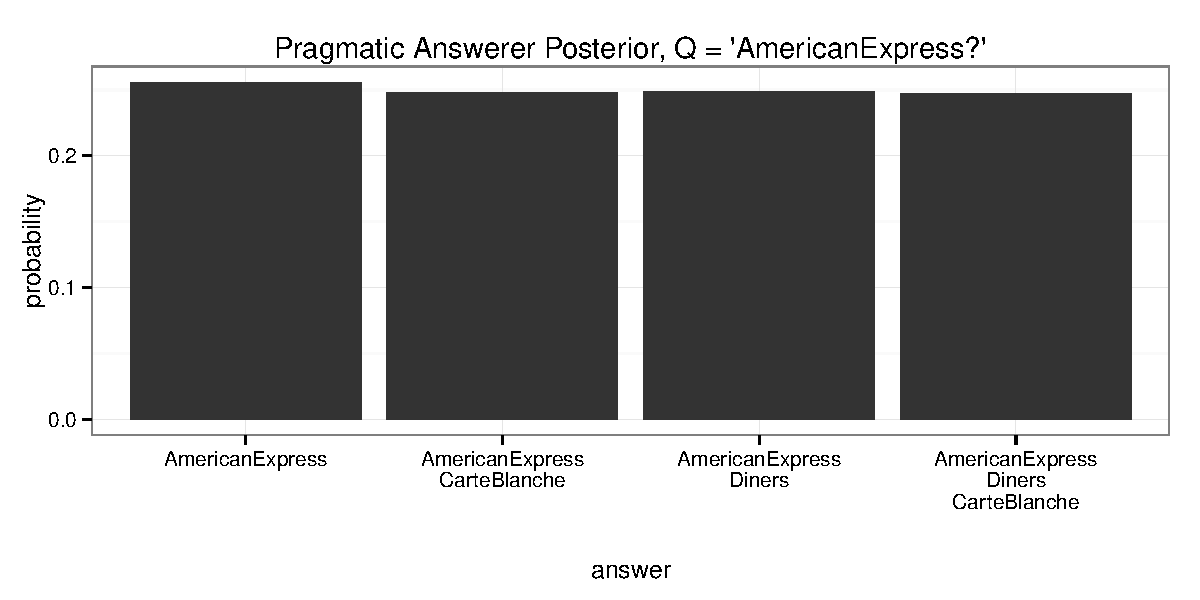
\includegraphics[scale = .6]{americanExpressPosterior.pdf}
%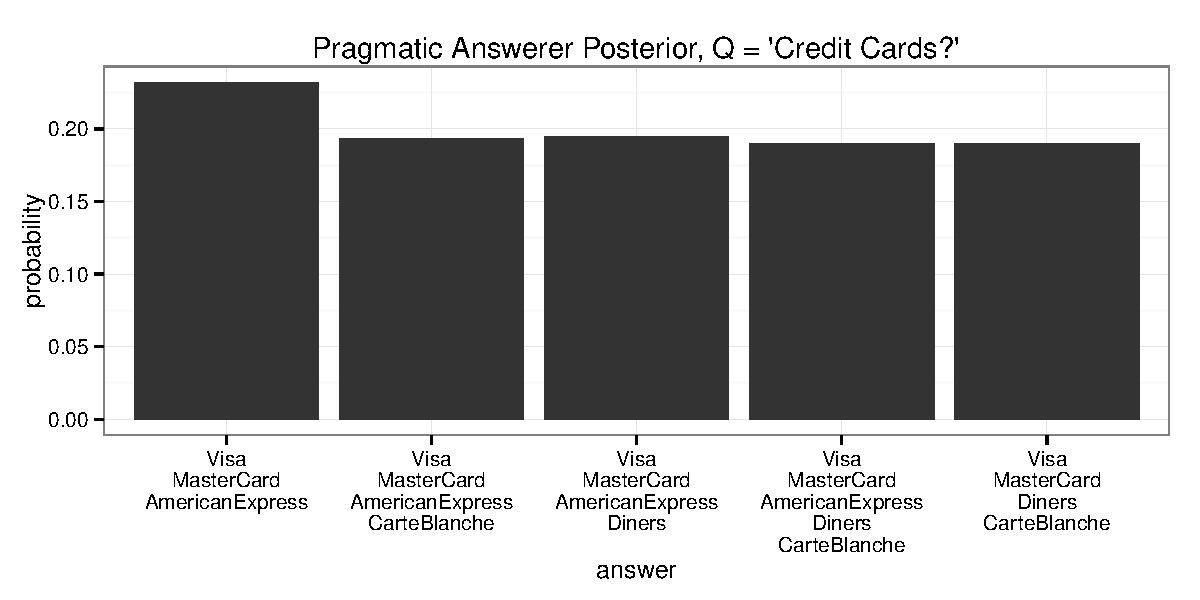
\includegraphics[scale = .6]{creditCardsPosterior.pdf}
%\end{center}
%\vspace{-.25cm}
%\caption{Comparison of questioner goal posteriors that the pragmatic answerer model infers after hearing two different question utterances in Clark (1979), Experiment 5. 
%\todo[inline]{There has to be a better way of presenting this result\dots}
%}
%\label{fig:clarkExperiment5posteriors}
%\end{figure*}

Because $A_0$ does not consider the question meaning, ``yes'' and ``no'' are not well-defined: the true list of cards is the most informative answer to any question, as it provides the exact identity of the true world. $A_1$, on the other hand, gives either a literal yes/no answer or exhaustive answer in proportion to their prior probability, regardless of which question is asked. Both answers provide complete information under the question projection.

By reasoning about the questioner's underlying goals, $A_2$ displays the pattern that \citeA{Clark79_IndirectSpeechActs} observed: a higher probability of giving a literal yes/no response to ``MasterCard?'' and ''American Express?'' than to "Credit cards?''. To understand \emph{why} $A_2$ behaves this way, we walk through the chain of pragmatic reasoning (Fig. \ref{fig:clarkExample}).

The key observation lies in the evidence provided by the question about the questioner's likely goal: $P(g | q) \propto P_{Q_1}(q|g)P(g)$. Consider two cases, beginning with the questioner's perspective  (left-most column of Fig. \ref{fig:clarkExample}). First, suppose $Q_1$ is only interested in an American Express card (goal $g_{\{AmEx\}}$). Any answer $A_1$ gives to $q_{AmEx}$ (the question ``American Express?'') would fully resolve her goal. ``Yes'' would yield certainty in accepting it and ``no'' in not accepting it. On the other hand, some answers to $q_{any}$ (``Credit cards?'') would not be resolving: if $A_1$ responded ``yes'', there would still be substantial uncertainty over whether the shop takes American Express in particular (for example, $A_1$ could informatively say ``yes'' if they only accepted Visa). A questioner with goal $g_{\{AmEx\}}$  is thus more likely to ask $q_{AmEx}$.


%We find that when the questioner asks ``Do you accept MasterCard?'', the pragmatic answerer gives a literal ``yes''/``no'' answer with probability $p = 0.92$ (compared to $p=1.00$ empirically). Similarly, when the questioner asks ``Do you accept American Express?'', the pragmatic answerer gives a literal answer with probability $p = 0.96$ (also compared to $p=1.00$ empirically). The small difference between these predicted response probabilities comes from the relative likelihoods of the different cards in the true world. However, when the questioner asks ``Do you accept credit cards?'', the probability of a literal response drops to $p = 0.76$ (compared to $p=0.73$ empirically). Our model output therefore provides a good fit to the original experiment data, both qualitatively and quantitatively.

%\todo[inline]{integrate this paragraph}
%Under the literal semantics of questions that $Q_1$ is assumed to be using, a negative answer to a more specific question (e.g. finding out that the store does not take MasterCard) would leave $Q_1$ with uncertainty about whether any of her other cards would be accepted. Meanwhile, both positive and negative answers to ``Credit cards?''  would be quite informative: a negative answer would leave her certain about  Knowing whether the shop takes \emph{any} cards (as opposed to no cards) is more informative than knowing whether or not they take a specific one. 


Now, suppose instead that $Q_1$ has a long list of cards (say, all five: $g_{all}$). A yes/no answer for any one card is not guaranteed to resolve her goal: if she asked $q_{AmEx}$ and got a ``no'', she is still uncertain whether another card on her list would be accepted. On the other hand, $q_{any}$ is expected to be highly informative under $A_1$; if she gets a ``no'', she is certain that no card on her list is accepted and if she gets a ``yes'', she is certain that one is. A questioner with goal $g_{all}$ is thus more likely to ask $q_{any}$.

This asymmetry in question behavior given different goals provides $A_2$ information about the goal given a question: he can invert this generative model to obtain a posterior $P(g | q)$ over goals (the center column of Fig.~\ref{fig:clarkExample} summarizes this goal distribution). By Bayes' rule, a singleton goal is more likely if the questioner asks $q_{AmEx}$ and a longer list of cards is more likely if she asks $q_{any}$. The latter goal is precisely the case where an exhaustive answer is most informative (left-most column of Fig.~\ref{fig:clarkExample}), thus leading to the empirical result: answerers are more likely to give indirect, exhaustive answers when asked ``Do you accept credit cards?'' 


%What makes $A_2$ \emph{pragmatic} is that the answerer will take into account the alternative questions a particular questioner \emph{could have} asked but didn't. Thus, a pragmatic answerer who hears the question ``Do you accept American Express?'' reasons that the questioner would have asked the other question if they were interested in a long list of cards. %Because they didn't ask that question, they must not have been interested in a long list of cards -- just American Express and perhaps a few less common cards (see Figure \ref{fig:clarkExperiment5posteriors}, top panel). The pragmatic answerer is then justified in preferring the resolving ``yes/no'' response; giving an exhaustive list of accepted credit cards is still a \emph{valid} answer, but useful only in a small number of worlds (e.g. where American Express is not accepted but Carte Blanche and/or Diner's card \emph{are} accepted).

% Similarly, when asked "Do you accept credit cards?'' the pragmatic answerer reasons that if the questioner were interested in a particular card $c$, they would have asked the more direct question ``Do you accept card $c$?'' and because they did not ask this question, it must not have been the goal. This inference also rules out goals where the questioner has one common card $c$ plus one or more rarer cards, since these goals also lead to the question ``Do you accept card $c$?'' With all these goals ruled out, we are left with five goals in which the caller has \emph{both} common cards (Visa and MasterCard) along with various other less common cards (see Figure \ref{fig:clarkExperiment5posteriors}, bottom panel). The answerer is uncertain as to which set of less common cards are owned. Thus, for any world where the restaurant does not accept Visa or MasterCard, an exhaustive list of accepted cards is determined to be the most informative answer on average. Note that these inferences are made purely on the basis of the questioner model's behavior under possible goals, rather than cues from context as in the previous simulations.

\subsection{Discussion}

In these case studies, we examined three empirical answerer-sensitivity effects that serve as desiderata for how a dialogue agent ought to interpret and respond to questions. 
They should be sensitive to the question utterance, the context, and the relationship between the questioner's goal and the utterance they produce to fulfill that goal.

A simple informative speaker $A_0$ was insensitive to all of these factors: it lacked a listener component that could induce any dependence on its partner's utterance. 
An informative answerer $A_1$ who also attempted to be \emph{relevant} with respect to the meaning of the question was sensitive to the question utterance, but it was unable to adapt its responses to different contexts or give more or less literal answers to different questions. 
Finally, a more sophisticated answerer $A_2$, who inferred the questioner's underlying goals and attempted to be directly relevant to those goals, qualitatively captured all three effects.
% in the same fashion \citeA{Clark79_IndirectSpeechActs} observed. %In the Appendix, we also show that only $A_2$ captures two additional answerer-sensitivity effects with similar characteristics from \citeA{GroenendijkStokhof84_SemanticsOfQuestions} and  \citeA{GibbsBryant08_OptimalRelevance}.

%can use these mechanisms to explain a range of sophisticated psycholinguistic phenomena, both qualitatively and quantitatively.

One concern with these results is that the answer distribution depends in each case on a stipulated space of alternative questions.
We chose simple, minimal sets to make the dynamics clear, but how robust are the results to the inclusion of additional alternatives?
To address this concern, we ran two additional analyses.
First, for our simulation evaluating sensitivity to context, we previously only included a single possible question (to isolate the effect of the context sentence).
Does this context effect disappear if a question directly corresponding to the other goal were available?
We re-ran our model after supplementing the set of possible questions with the alternative ``How much does a fifth of Jim Beam cost?'' which we assigned a literal meaning that is identical to the exact price goal, $g_{=}$.
We found that the existence of this alternative does slightly reduce the answerer's preference for responding with the exact price (from 62\% to 60\%, because $A_2$ reasons that if $Q_1$ really cared about the exact price, they would have asked this other question), but it has the same effect for the other context sentence, leaving the qualitative context effect unchanged.
%As the rationality parameter increases, this effect increasingly overwhelms the effect of the context prior, but 
\ndg{does this depend on cost of the new question? if so indicate, if not delete me.}

A similar question arises in the credit card scenario: if the most direct question, ``What cards do you accept?'', was a potential alternative, would it interfere with the answerer's sensitivity to the questions they were asked?
To explore this, we assigned this question a literal meaning that projects the world to the exact list of cards that are accepted and re-compute $A_2$'s behavior.
Again, we found that the qualitative effect of interest was robust to this change. 
%The key insight for understanding why lies in the observation that this question is good for all goals. 
Because $Q_1$ will consider this a good question regardless of their goal, failing to ask it is not particularly informative about the goal: the more informative signal, for $A_2$, about the goal is provided by the \emph{relative differences} in preferences for the other questions, which roughly puts us back in the case when we did not include this question in the set of possibilities.
We conclude that, at least in the most obviously worrisome cases, our model's qualitative pattern of behavior does not change with larger spaces of question alternatives, although the effect size may differ.
%Because the precise numerical output was already sensitive to the rationality parameters and numerical choices of answer costs, we .
%Our aim in these simulations was not to fit exact values but to demonstrate how qualitative effects emerge in the $A_2$ model.
% and the mathematical form of the various priors

%We set these components to be simple and natural in the context of the scenario being modeled, but there is still some concern over the amount of flexibility afforded to the modeler in making these choices. For example, the answer prior for both Clark studies uses a parameter to determine the answerer's baseline preference for `yes' and `no' responses versus prices or lists of card types. In both cases we set this parameter to be $p = 0.5$, but other numbers could have been chosen to achieve a better or worse quantitative fit. 

These case studies focus on answerer behavior and demonstrate how social reasoning explains prior experimental findings in a unified formal framework. 
However, our framework also generates novel predictions not addressed by existing experimental data.
Most conspicuously, there is a relative lack of data on how people \emph{choose questions} in the similar social scenarios---when the questioner knows her partner wants to be helpful but may not know ahead of time exactly what goal she is pursing.
We therefore designed a new experimental paradigm---the \emph{Hidden Goal} paradigm---to simultaneously probe questioner and answerer behavior under such conditions.
This paradigm allows us to rigorously compare our different models, and to empirically justify our modeling assumptions.

\section{The Hidden Goal paradigm}

The functional motivations for asking (epistemic) questions lie in two sources of informational asymmetry. 
Agents have both (1) private goals and (2) private knowledge about the world. 
If the questioner already knew the relevant information about the world, there would be no need to ask about it.
Similarly, if a cooperative answerer already knew the questioner's goal, they would just provide the necessary information without needing to hear a question.
Thus, studying how people ask and answer questions in dialogue requires an experimental paradigm that can induce and manipulate these two forms of uncertainty.

Prominent paradigms for studying question asking in the lab, including \emph{Battleship} \cite{RotheEtAl16_NaturalLanguageQuestions, rothe2018people} or \emph{20 Questions}-style games \cite{Siegler77_TwentyQuestions, cohen2016searching, NelsonDivjak___Meder14_GuessWho, RuggeriEtAl15_HierarchicalTwentyQs}, have been ideal for investigating how people select between different possible queries.
By withholding from the questioner the ground truth location of the ships in \emph{Battleship}, or the identity of the object that their partner is thinking of in \emph{20 Questions}, they effectively induce an asymmetry in knowledge about the world.

However, by design, the answerer in these paradigms knows the questioner's true goal with certainty (e.g. to ``find all battleships'') and is constrained to respond truthfully but otherwise uncooperatively.
This simplification---fixing a single goal and limiting the expected behavior of the answerer---is desirable for measuring question preferences over large, unbounded spaces \cite{cohen2016searching, rothe2017question} or probing developmental change in basic informational search \cite{RuggeriEtAl15_HierarchicalTwentyQs, ruggeri2016sources}, but severely limits the pragmatic interplay that is characteristic of real-world dialogue. 

\begin{figure*}[t!]
\begin{center}
\includegraphics[scale = .89]{Exp1/Exp1Task.pdf}
\end{center}
\caption{\footnotesize Task display and procedure for Experiment 1. (A) Questioner is privately assigned a goal object to find, but does not know which objects are behind which doors; answerer is privately shown the locations of objects but does not know which object the questioner is trying to find. Possible questions are shared. (B) Example of a single trial proceeding through 4 phases: goal assignment, question selection, answer selection, and location guess.}
\label{fig:expviews}
\end{figure*}


We propose the \emph{Hidden Goal} paradigm to address the challenge of creating the functional conditions for question and answer pragmatics in a controlled lab setting.
There are two key features that distinguish this paradigm from those used in prior work.
First, while preserving the asymmetry in world knowledge between questioner and answerer used in prior work, it also explicitly introduces an asymmetry in access to \emph{goals}.
We privately assign one of several possible goals to the questioner and withhold information about the identity of this goal from the answerer. 
Second, it establishes a \emph{joint task} shared by both participants---the answerer is only rewarded when the questioner meets their goal---thus creating the need for cooperation in combining these different sources of private knowledge. 

%First, while our case studies were drawn from extensive experimental work on \emph{answerer} behavior, data on questioner pragmatics is scare.
% directly tested whether people behave as the questioner models predict, or compared the different levels of questioner models against one another. 
% To do so, we must collect data on which question a questioner prefers to ask given a particular goal. 
%Second, we must provide empirical evidence for the assumptions we make about internal model choices: for instance, the priors and spaces of alternative questions, answers, or goals in a particular scenario. 
%Finally, validate the predicted goal inference. 

%To satisfy these three requirements, we designed a reference game to simultaneously collect data on question-asking behavior \emph{and} answering behavior in interaction, carefully controlling or measuring priors and utterance sets. 
%Since \citeA{Wittgenstein09_PhilosophicalInvestigations}, reference games have provided a simple but productive testbed for eliciting pragmatic behavior: one participant must choose an utterance to communicate the identity of a target object to their partner in a shared context. 

In the remainder of the paper, we present three behavioral experiments in this paradigm that provide a more rigorous evaluation of both questioner and answerer models in our framework.
Each experiment additionally demonstrates how the core computational mechanisms of our theory can be elegantly composed with other linguistic and cognitive primitives to capture more sophisticated question and answer behaviors.
In Exp.~1, we extend our model with an underlying formal account of definite reference in questions (e.g. ``where is \emph{the} dog?'') which uses graded knowledge of concept typicality.
In Exp.~2, we show how the model extends to hierarchically structured spaces of goals.
And finally, in Exp.~3, we show how the same framework straightforwardly extends to multi-round dialogue, where the answer to one question affects the next.

\section{Experiment 1: \\ Definite reference and conceptual knowledge}

%%%
As a first quantitative test of our models, we designed a cooperative guessing game that relies on knowledge of concept structure. \ndg{"concept structure" is kind of vague.. maybe something like ontological relations (e.g. a dalmatian is a dog)?}
% This game served as a minimal case of the Hidden Goal paradigm.
On each trial, four objects are hidden behind four doors.
One player -- the \emph{questioner} -- is assigned one of the objects to find as a private goal but does not know which object is behind which door.
The other player -- the \emph{answerer} -- knows each object's true location but does not know which one the questioner is looking for (Fig. \ref{fig:expviews}A). 
To succeed in the face of this knowledge asymmetry, the questioner must first ask a question (i.e. \emph{where is the\dots?}), then the answerer must respond helpfully so that the questioner can guess the location of their goal object more accurately (Fig. \ref{fig:expviews}B).

Critically, we manipulated the sets of goals, questions, and answers across trials to create a number of different scenarios where our models make distinguishable predictions.
To do so, we exploited the hierarchical conceptual structure provided by nominal referring expressions.
For example, a questioner could ask about the ``Dalmatian,'' ``dog,'' ``pet,'' or ``animal'' and all could plausibly describe an image of a Dalmatian in the answerer's view \cite{Brown58_HowShallAThingBeCalled,GrafEtAl16_BasicLevel}. 
However, among these labels, only the super-ordinate label ``animal'' could describe an image of a whale.
These conceptual relationships interact with common knowledge of alternative questions and answers to license different pragmatic inferences.

\begin{figure*}[th!]
\begin{center}
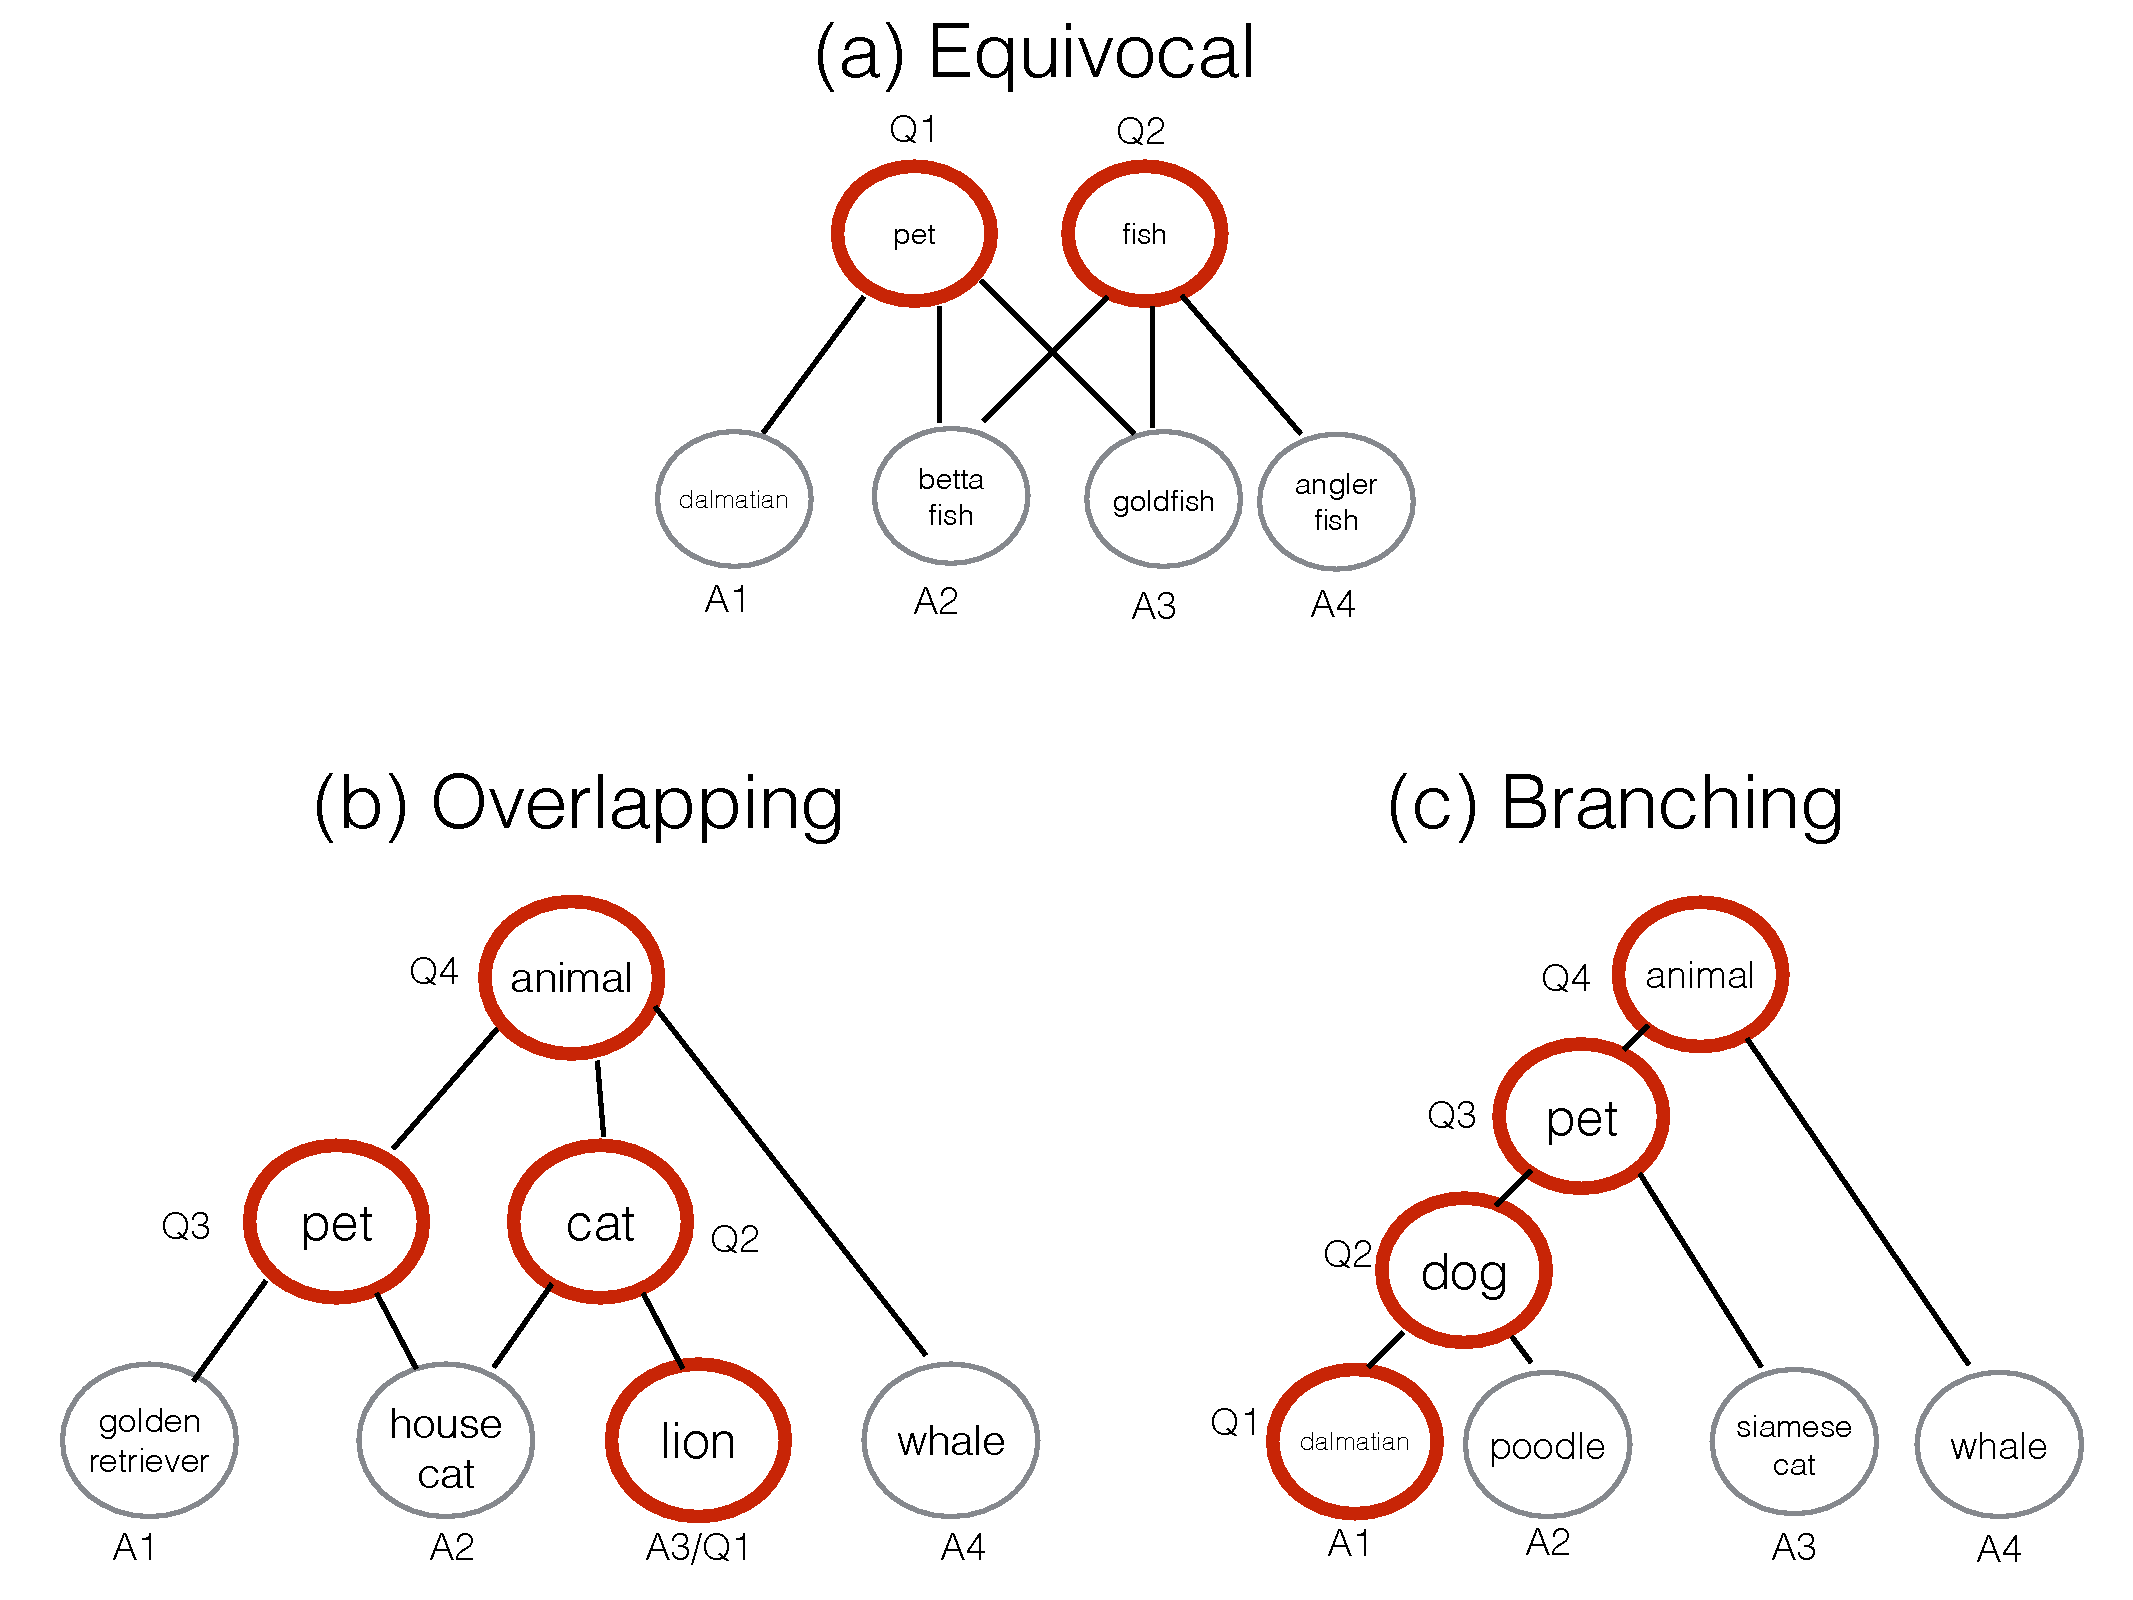
\includegraphics[scale = .5]{Exp1/hierarchyStructureExamples.pdf}
\end{center}
\caption{\footnotesize  Example of each condition of conceptual hierarchy used in our experiment. Example stimuli are shown for the \emph{animals} domain, but the other conceptual domains were structurally identical.}
\label{fig:hierarchyStructures}
\end{figure*}

\subsection{Methods}
\subsubsection{Participants} 
200 participants from Amazon's Mechanical Turk were recruited and paired into teams of two.
We excluded 50 participants due to a server crash that terminated the task before completion, and
excluded two additional games because participants reported that they were not native English speakers. 
This left 74 unique completed games (148 participants).

\subsubsection{Stimuli} 

To support quantitative model comparison, we needed to elicit graded behavior under a variety of different scenarios.
We thus constructed twelve items by crossing four conceptual domains (\emph{animals}, \emph{plants}, \emph{places}, and \emph{artifacts}) with three concept hierarchy structures (\emph{nested}, \emph{overlapping}, and \emph{equivocal}; see Figure \ref{fig:hierarchyStructures}).
Each item consisted of four objects and four labels, such that different labels referred to different subsets of objects at different levels of abstraction. 
The four objects served as possible goals and answers, while the labels served as possible questions\footnote{A document containing these stimuli for all items is available online at \scriptsize\url{https://osf.io/cjs85/}}.
The different concept hierarchy structures were intended to serve as conditions driving qualitatively different model predictions, while the conceptual domains were intended to support item-level generalizability within each condition (i.e. to ensure that a particular idiosyncratic choice of images or labels is not driving the effect).

%The objects in context on a given trial belong to a conceptual hierarchy (see Fig. \ref{fig:hierarchyStructures} for several examples).
%As discussed in detail below, our models make qualitatively and quantitatively different predictions about (1) which of these levels the questioner will choose in different contexts and (2) how answerers will respond to underspecified questions like ``Where is the dog?'' when there are multiple dogs in context.

\subsubsection{Procedure}

\begin{figure*}[tbh]
\begin{center}
\includegraphics[scale = .9]{Exp1/QualitativePredictions.pdf}
\end{center}
\caption{\footnotesize  Qualitative model predictions and results for (A) answerers in nested condition and (B) questioners in overlapping condition. Highlighted rows indicate clearest qualitative differences. Response counts are aggregated across the conceptual domains.}
\label{fig:exp1qualitative}
\end{figure*}

After passing a short comprehension quiz on the game instructions, participants were randomly assigned to the role of questioner or answerer and paired with another participant in a shared virtual environment using the infrastructure described in \citeA{Hawkins15_RealTimeWebExperiments}. 
Some aspects of each participant's environment were denoted as private (i.e. the questioner's goal and the answerer's knowledge of object locations) while others were explicitly flagged as common ground (i.e. the sets of possible questions and objects).
%The questioner and answerer interfaces are displayed in Figure \ref{fig:expviews}. %Information was presented on the left side of the screen, and players used the right side as a workspace to view goals, ask questions, and respond with answers. 
%It was important to sets were presented alternatives are fixed and held in common ground for all participants. 
Fixing these sets and making them explicit as common ground allowed us to avoid ad hoc assumptions about these sets in our model formulation, and also reduced the memory load on participants.


We constructed the trial sequence such that each participant provided one response for each of the twelve items, in a random order.
Each trial proceeded through four phases. 
First, the questioner was randomly assigned one of the four possible goals by a spinning wheel animation.
They then used a drag-and-drop interface to select one of the four questions to send.
Upon seeing this question appear, the answerer responded with a location (``The X is behind door Y'') by dragging the object they wanted to reveal into a box. 
Each of these drag-and-drop actions was rendered for the other participant in real time to emphasize that they were playing with a real human partner.
Finally, after receiving the answer, the questioner clicked on one of the gates to make their guess. 
Both players received feedback about the outcome of the guess: the questioner saw the true locations of the objects, and the answerer saw the questioner's true private goal. 

\subsection{Qualitative results}

Before proceeding to quantitative model comparisons, we highlight several key patterns in the behavioral data where models make qualitatively different predictions. 
This allows us to \emph{falsify} certain models on the basis of failing to predict these qualitative patterns \cite{palminteri2017importance}.
Because these predictions are based purely on the hierarchy structures, we treat the four domains as distinct items in our analyses but continue using examples from the ``animal'' domain for readability.

\subsubsection{Answerer behavior}
The most straightforward qualitative prediction distinguishing our answerer models concerns the \emph{nested} condition. 
This condition was characterized by four successively more specific labels, ranging from the super-ordinate ``animal'' to the sub-ordinate ``Dalmatian.'' 
At each layer of conceptual nesting, one of the objects in context was excluded: ``animal'' is true of all four objects, ``pet'' is true of three, and so on.
The aggregated answerer response distribution across domains is shown for all possible questions in Fig.~\ref{fig:exp1qualitative}A.

Some answerer behavior is straightforwardly predicted by both $A_1$ and $A_2$: when asked ``Where is the \emph{Dalmatian}?'', 100\% of participants revealed the location of the Dalmatian.
Other questions, however, lead to sharp qualitative differences between models.
Suppose the questioner asks ``Where is the \emph{animal}?''. 
Neither $A_0$ nor $A_1$ have a preference over which of the animals to provide information about, because all four satisfy the literal meaning of the question. 
Human participants, on the other hand, displayed a strong preference across domains: 94\% provided the location of the ``whale,'' the object that isn't queried by any of the other questions.

We statistically tested the non-uniformity of this distribution while accounting for domain-level variability by running a log-linear mixed-effects model with random effects for domain\footnote{Because of the small number of responses per participant, we were unable to also estimate participant-level random effects. We considered controlling for domain more important, however --- although there high agreement in responses across domains overall, the `place' domain was a notable outlier due to a confusing choice of images (see Appendix Table 1).}. 
Specifically, we used a Poisson linking function to predict the (log) count data for each response level, as implemented in \texttt{lme4} \cite{bates2014fitting}.
Our null model contained only a fixed intercept, and random intercepts for each domain, capturing the qualitative prediction of $A_0$ and $A_1$ that all response levels share the same frequency.
We compared this to an alternative model adding an additional regressor that was dummy-coded 1 for ``whale'' and 0 for the other levels, allowing flexibility to break the symmetry.
Because these models are nested, we used a likelihood-ratio test comparison accounting for additional degrees of freedom. 
We found that the intercept-only model was strongly rejected in favor of the non-uniform model, $\chi^2(3) = 181, p < 0.001$.
%Most simply, we collapsed response counts across the domains and conducted a chi-squared goodness of fit test, finding significant deviation from a uniform distribution, $\chi^2(3) = 210.8, p < 0.001$ (see Fig. \ref{fig:exp1qualitative}A).

This non-uniform pattern is only consistent with the predictions of $A_2$. 
To understand why, consider the inference that can be made about the underlying goal from hearing the utterance ``Where is the animal?''.
$A_2$ reasons that if the questioner were looking for the Dalmatian, they would be more likely to ask ``Where is the Dalmatian?''. 
If looking for the other dog, the poodle, they would have asked ``Where is the dog?''
More generally, they would have been more likely to ask a more direct question under any goal except the ``whale,'' and the fact that they \emph{didn't} ask one of these more direct questions is evidence that they didn't have these goals.
Having inferred that the most likely goal is the whale, $A_2$ gives the most informative, relevant answer: the location of the whale.

\subsubsection{Questioner behavior}
Next, we turn to a subtler qualitative pattern in the ``overlapping'' condition, which was designed to distinguish between our \emph{questioner} models. 
The aggregated counts of participants asking each possible question in this condition are shown in Fig. \ref{fig:exp1qualitative}B. 
One goal in particular leads to qualitatively diverging predictions across models: suppose the questioner is assigned the ``house cat'' as their goal object (the row highlighted in green). 
$Q_0$ is equally likely to ask any of the four questions in this scenario, since $A_0$ ignores their utterance anyway. 
$Q_1$, in turn, is evenly split between the two parents in the tree -- ``Pet?'' and ``Cat?'' --- it reasons that $A_1$ would have a 50\% chance of responding with the house cat's location in either case. 
Empirically, we observed that 64\% of questioners asked ``Cat?'' while only 25\% asked ``Pet?''

We again used a mixed-effects regression model to account for domain-level variability when testing whether these probabilities deviated from uniform.
Our simplest model only contains a fixed intercept, forcing all responses to be generated from the same parameter.
Our second model, representing $Q_1$'s qualitative predictions, adds a categorical predictor coded 1 for ``Cat?'' and ``Pet?'' and -1 for the other two responses, thus forcing the former two responses to share a single parameter.
Our final model added an orthogonal contrast allowing ``Cat?'' and ``Pet?'' to be different (i.e. 1 for ``Cat?'', -1 for ``Pet?''). 
All of these models contained domain-level random effects for each fixed-effect regressor.
We found in a nested likelihood-ratio test that the second model was significantly preferred to the intercept-only model, $\chi^2(3) = 49, p < 0.001$, but that the third model allowing the ``Cat?'' and ``Pet?'' to differ was significantly preferred over the model forcing them to be the same, $\chi^2(4) = 26, p < 0.001$.
This allows us to falsify $Q_0$ and $Q_1$ because they fail to capture this qualitative asymmetry.

$Q_2$, on the other hand, successfully predicts this asymmetry (see Fig. \ref{fig:exp1qualitative}B) because it takes into account the goal inferences $A_2$ would make after hearing her question. 
Once $A_2$ hears ``Cat?'' he will infer, using the same Gricean logic described above, that because the more specific ``Lion?'' is an available alternative for the questioner, she would have \emph{directly} asked about it if it were her goal. 
Because she didn't, he infers that she must be interested the other cat (her true goal). 
``Pet?'' on the other hand, gives no clue to her goals and is therefore less preferred. 
This critical condition thus provides qualitative evidence for $Q_2$: in some cases, questioners consider the answerer's inference about their goals when selecting their question. 

%
%\begin{figure}[t!]
%\begin{center}
%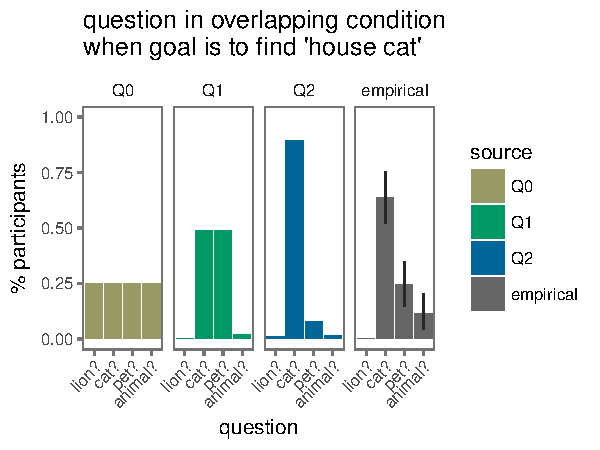
\includegraphics[scale=.9]{OverlappingModelComparison.pdf}
%\end{center}
%\caption{.}
%\label{fig:Exp4ZoomedIn}
%\end{figure}


%We find that the pragmatic model $Q_2$ makes the correct qualitative prediction -- the empirical probability of asking ``Cat?'' ($\hat{p} = 0.64$) is significantly different from the  probability of asking ``Pet?'' ($\hat{p} = 0.25$; bootstrapped $95\%$ CI on difference: $[0.17, 0.58]$). 

%Thus, in examining the results below we will collapse across domains for simplicity of analysis. 
%Still, it is worth noting that the ``place'' domain has the lowest inter-domain correlations for both questioners and answerers, indicating that it may be an outlier -- we will return to this point in the discussion below.  Next, we step through the response patterns for each hierarchy type. For concreteness, though all statistical tests were conducted on data pooled across domains, we report our results in terms of the `animal' domain instead of the abstract goal, question, and answer labels (see Figure \ref{fig:exp4res} for the full response distributions).
%
%\begin{figure*}[t!]
%\begin{center}
%\includegraphics[scale = .75]{Exp2QuestResults}
%\includegraphics[scale = .75]{Exp2AnsResults}
%\end{center}
%\caption{Results and model fits, for the best-performing questioner (left) and answerer (right) models, collapsing over the different domains. Error bars represent bootstrapped 95\% confidence intervals.\todo[inline]{Judith: axes difficult to read. Maybe just use animal labels here? Or move to supplemental?}}
%\label{fig:exp4res}
%\end{figure*}

%In the `overlapping' condition (Figure \ref{fig:hierarchyStructures}(b)), questioners preferentially asked about the `lion' when looking for the lion, $\chi^2(3) = 205, p < 0.001$; about the `cat' when looking for the Siamese cat, $\chi^2(3) = 63, p < 0.001$, even though the lion is also a cat; about the `pet' when looking for the dalmatian, $\chi^2(3) = 232, p < 0.001$, even though the Siamese cat is also a pet; and about the `animal' when looking for the whale, $\chi^2(3) = 213, p < 0.001$. Answerers preferentially revealed the lion when asked about the `lion,' $\chi^2(3) = 229, p < 0.001$, the Siamese cat when asked about the `cat,' $\chi^2(3) = 59, p < 0.001$, the dalmatian when asked about the `pet,' $\chi^2(3) = 120, p < 0.001$, and the whale when asked about the `animal,' $\chi^2(3) = 187, p < 0.001$. 

%In the `branching' hierarchy (Figure \ref{fig:hierarchyStructures}(c)), we found that questioners strongly prefer to ask about the `dalmatian' when trying to find the dalmatian, $\chi^2(3) = 190, p < 0.001$, about the `dog' when trying to find the poodle, $\chi^2(3) = 152, p < 0.001$, about the `pet' when trying to find the siamese cat, $\chi^2(3) = 168, p < 0.001$, and about the `animal' when trying to find the whale, $\chi^2(3) = 210, p < 0.001$. %Answerers respond in kind. , and in an earlier version of the multi-player study we report in this section.

To summarize, our non-pragmatic models cannot account for key qualitative phenomena while our pragmatic models ($A_2$ and $Q_2$) make the correct predictions. 
Next, we show that our pragmatic models also provide better overall quantitative fits to the raw behavioral data. 
Before describing the results of our model comparison, we formalize the task setup in our modeling framework. 

\subsection{Quantitative model comparison}


% Please add the following required packages to your document preamble:
% \usepackage{booktabs}
% \usepackage{multirow}

\subsubsection{Setup} 
Corresponding to the structure of our experiment design, we take the set of possible worlds $\mathcal{W}$ on a given trial to be the set of possible permutations of the four objects to the four locations (yielding $4! = 24$ possibilities). 
Because we explicitly instructed questioners to find the location of a particular object, we then take the space of goals $\mathcal{G}$ to be the set of goal projections $$g_o(w) = \textrm{loc}(o,w)$$ where $\textrm{loc(o,w)}$ is a simple function looking up the location of object $o$ in world $w$. 
Similarly, the answer space $\mathcal{A}$ is the set of constructions ``The $o$ is behind gate $i$.'' which evaluate to true in worlds where $o$ is at location $i$ and false otherwise.
We assume uniform prior probability over worlds, goals, questions, and answers. 

%The formal semantics of the questions in our experiment  several classic problems in linguistics.
%The semantics of questions in this domain is 
%To populate our question space $\mathcal{Q}$, we must specify the explicit meaning of the question ``Where is the $x$?'' for each of the four labels allowed in a given trial (see Fig. \ref{fig:hierarchyStructures}). 
Specifying the formal semantics of the question space $\mathcal{Q}$ draws upon ideas from linguistics. 
The denotation of a noun phrase containing a definite article is only defined if there is a unique, salient object that the noun picks out in the world; pragmatically, the use of a definite article \emph{presupposes} the uniqueness or identifiability of some object in shared context \cite{Lewis79_Scorekeeping, clark1983common, Roberts03_UniquenessDefiniteNounPhrases}. 
Thus we take the meaning of each question $q$ to be: 
$$\textrm{\den{Where is the x?}} = q_{x}(w) = i_x$$ where $i_x$ is the \emph{identifiable} object of category $x$. 
In contexts where there are multiple objects of category $x$, the definite article is interpreted by sampling an object from a prior identifiability distribution over objects in the labelled category: $i_x \sim \mathcal{I}(o | x)$. 
This distribution may depend on distinctive visual properties, the typicality of the object for the category \cite{Rosch75}, world knowledge about which labels people tend to use to refer to different objects, and other information in common ground \cite{ClarkMarshall1981}.
To estimate the combined weight of these influences on interpretation, we estimated the empirical identifiability prior from an independent elicitation task.

\subsubsection{Eliciting empirical identifiability priors}
In prior work, there have been two approaches to setting model-internal prior distributions in a principled manner.
The first is to treat these internal distributions as additional free parameters and jointly infer them from the behavioral data along with other parameters of interest \cite<e.g.>{TesslerGoodman16_Generics, tauber2017bayesian}. 
The second is to use an independent task to empirically elicit these priors from a separate population of participants, and then use this (parameter-free) distribution in the model \cite<e.g>{KaoWuBergenGoodman14_NonliteralNumberWords}.
Here, we take a hybrid approach. 
We elicit empirical identifiability priors from an external sample, as in the second approach, but then infer the extent to which these empirical priors are actually necessary for explaining participants' question and answer behavior in our model comparison.

We thus designed a simple elicitation task using the stimuli from our communication task.
On each trial, we presented participants with a set of four pictures and a label $X$ and were asked to ``Click \emph{the} $X$.''
Each participant was given one trial for each of the twelve items used above; to obtain the label $X$, we sampled one of the four possible category nouns that could be used in questions. 
In this way, no participant saw the same set of objects more than once. 
%The order of trials and positions of pictures within trials were randomized.
Of 192 participants recruited from Amazon's Mechanical Turk, 13 participants were excluded after reporting a non-English native language, and 15 more were excluded due to self-reported confusion over the instructions. 
This left data for 164 participants.
To form an empirical identifiability distribution $\mathcal{I}(o | x)$ that can be used in the model, we computed the proportion of participants that clicked on each of the objects $o$ for each label $x$. 

Before formally testing the importance of these empirical priors in our model comparison, we conducted a simple test of the null hypothesis that participants use a uniform prior over within-category objects when interpreting the definite article. 
We performed Pearson $\chi^2$ goodness of fit tests on the response distribution for each label: a total of 32 tests. 
We found that 69\% of these tests rejected the null hypothesis of uniformity at a (Bonferroni-corrected) significance level of $\alpha = 0.05/32 = 0.002$ indicating that the identifiability distribution often deviates from uniform: not all members of a category are equally likely to be identified as the referent of the definite description.

\subsubsection{Results of model comparison}

%How does correcting this assumption affect our quantitative model predictions? 
%The empirical saliency distributions we collected can be directly substituted in for $\mathcal{S}(o|x)$ when defining the literal semantics of ``Where is \emph{the}\dots?'' questions. 


%We assume uniform prior probability over worlds, goals, questions, and answers. 
%This finishes the specification of the three Questioner models and three Answerer models for our experimental situation.
For a rigorous model comparison among our different questioner and answerer models, we conducted a Bayesian data analysis \cite{LeeWagenmakers14_BDA}. 
First, because utterances did not differ in cost, we remove the cost term of the model for simplicity by setting $\beta=0$.
%We introduce a discrete hyperparameter $\gamma \in \{0, 1, 2\}$  determining which model to use, and jointly infer this parameter along with the continuous rationality parameter $\alpha$.
Additionally, to test whether a model using our empirically-measured identifiability prior provides a better fit to the data than a uniform prior, we add an additional parameter $w \in [0,1]$ which interpolates between them.
In other words, we assume participants use some mixture between the pure uniform \ndg{uniform over objects consistent with noun? clarify.} and empirical priors but we have uncertainty over the mixture weight.
We place uninformative priors over these parameters,
$\alpha_A   \sim  \textrm{unif}(0,40)$, 
$\alpha_Q   \sim  \textrm{unif}(0,40)$, 
$w \sim \textrm{unif}(0, 1)$.

We estimated the marginal likelihood of our raw answerer data under $A_0$, $A_1$, and $A_2$, and of our questioner data under $Q_0$, $Q_1$, and $Q_2$.
Additionally, for each of these models, we constructed a lesioned variant that did not use the empirical identifiability priors (i.e. $w=0$).
Our model comparison thus includes six questioner models and six answerer models.
To estimate marginal likelihoods, we used annealed importance sampling \cite<AIS;>{neal2001annealed} and averaged estimates across 16 chains of 10,000 MCMC steps each to obtain stable estimates for each model. 

%After marginalizing over values of $\alpha$ and $w$, the posterior $P(\gamma | \textrm{data})$ can be interpreted as the relative evidence for each model \cite{KruschkeVanPaemel15_OxfordHandbook}.
Results of our model comparison are shown in Table \ref{tab:exp1likelihoods}. 
We can immediately rule out $A_0$ and $Q_0$, which predict a uniform distribution of responses within each condition and performed many orders of magnitude worse than the other models.
Among the remaining full answerer models, we found overwhelming evidence for $A_2$ relative to $A_1$ (BF~$\approx~4~\times~10^{92}$).  
For our full questioner models, we found substantial evidence for $Q_2$ relative to $Q_1$ (BF~$\approx4\times~10^{7}$). 


\begin{table}[]
\begin{center}
\begin{tabular}{@{}llrr@{}}
\toprule
 &  & \multicolumn{1}{l}{\begin{tabular}[c]{@{}l@{}}uniform\\ identifiability\end{tabular}} & \multicolumn{1}{l}{\begin{tabular}[c]{@{}l@{}}empirical\\ identifiability\end{tabular}} \\ \midrule
\multirow{3}{*}{\begin{tabular}[c]{@{}l@{}}answerer\\ models\end{tabular}} & $A_0$ & -1231.0 & -1231.0 \\ \cmidrule(l){2-4} 
 & $A_1$ & -848.5 & -767.6 \\ \cmidrule(l){2-4} 
 & $A_2$ & -587.9 & \textbf{-554.3} \\ \midrule
\multirow{3}{*}{\begin{tabular}[c]{@{}l@{}}questioner\\ models\end{tabular}} & $Q_0$ & -1025.9 & -1025.9 \\ \cmidrule(l){2-4} 
 & $Q_1$ & -344.2 & -329.3 \\ \cmidrule(l){2-4} 
 & $Q_2$ & -342.9 & \textbf{-311.8} \\ \bottomrule
\end{tabular}
\vspace{1em}
\end{center}
\caption{\footnotesize Results of quantitative model comparison for Exp.~1; marginal likelihoods shown on log scale.}
\label{tab:exp1likelihoods}
\end{table}


Next, having established support for $A_2$ and $Q_2$, we examine their lesioned variants to test whether the introduction of empirical identifiability distributions improved our predictions. 
Again using Bayes Factors, which automatically penalize our full model for its additional flexibility, we found strong evidence against the $w=0$ model for both the answerer (BF~$\approx4\times~10^{14}$) and questioner ($3.2 \times 10^{13}$), suggesting that participants account for non-uniform knowledge about salience and conceptual typicality when interpreting the definite article.

Finally, to examine parameter posteriors and predictives for each model, we performed inference using MCMC.
We used a burn-in of 4000 steps and lag of 12 to obtain 500 posterior samples for each model.
We find that the posterior predictives for the best-fitting answerer and questioner models explain a substantial proportion of the item-wise variance across domain and hierarchy type: $R^2 = .92$ and $R^2 = .98$, respectively (see Fig. \ref{fig:exp1predictives}). 
The MAP parameters are $\alpha_A = 36, \alpha_Q = 6, w = 0.4$ for the best performing questioner model and $\alpha_A = 3.5, \alpha_Q = 21, w = 0.6$ for the best-performing answerer model.

\begin{figure*}[tb]
\begin{center}
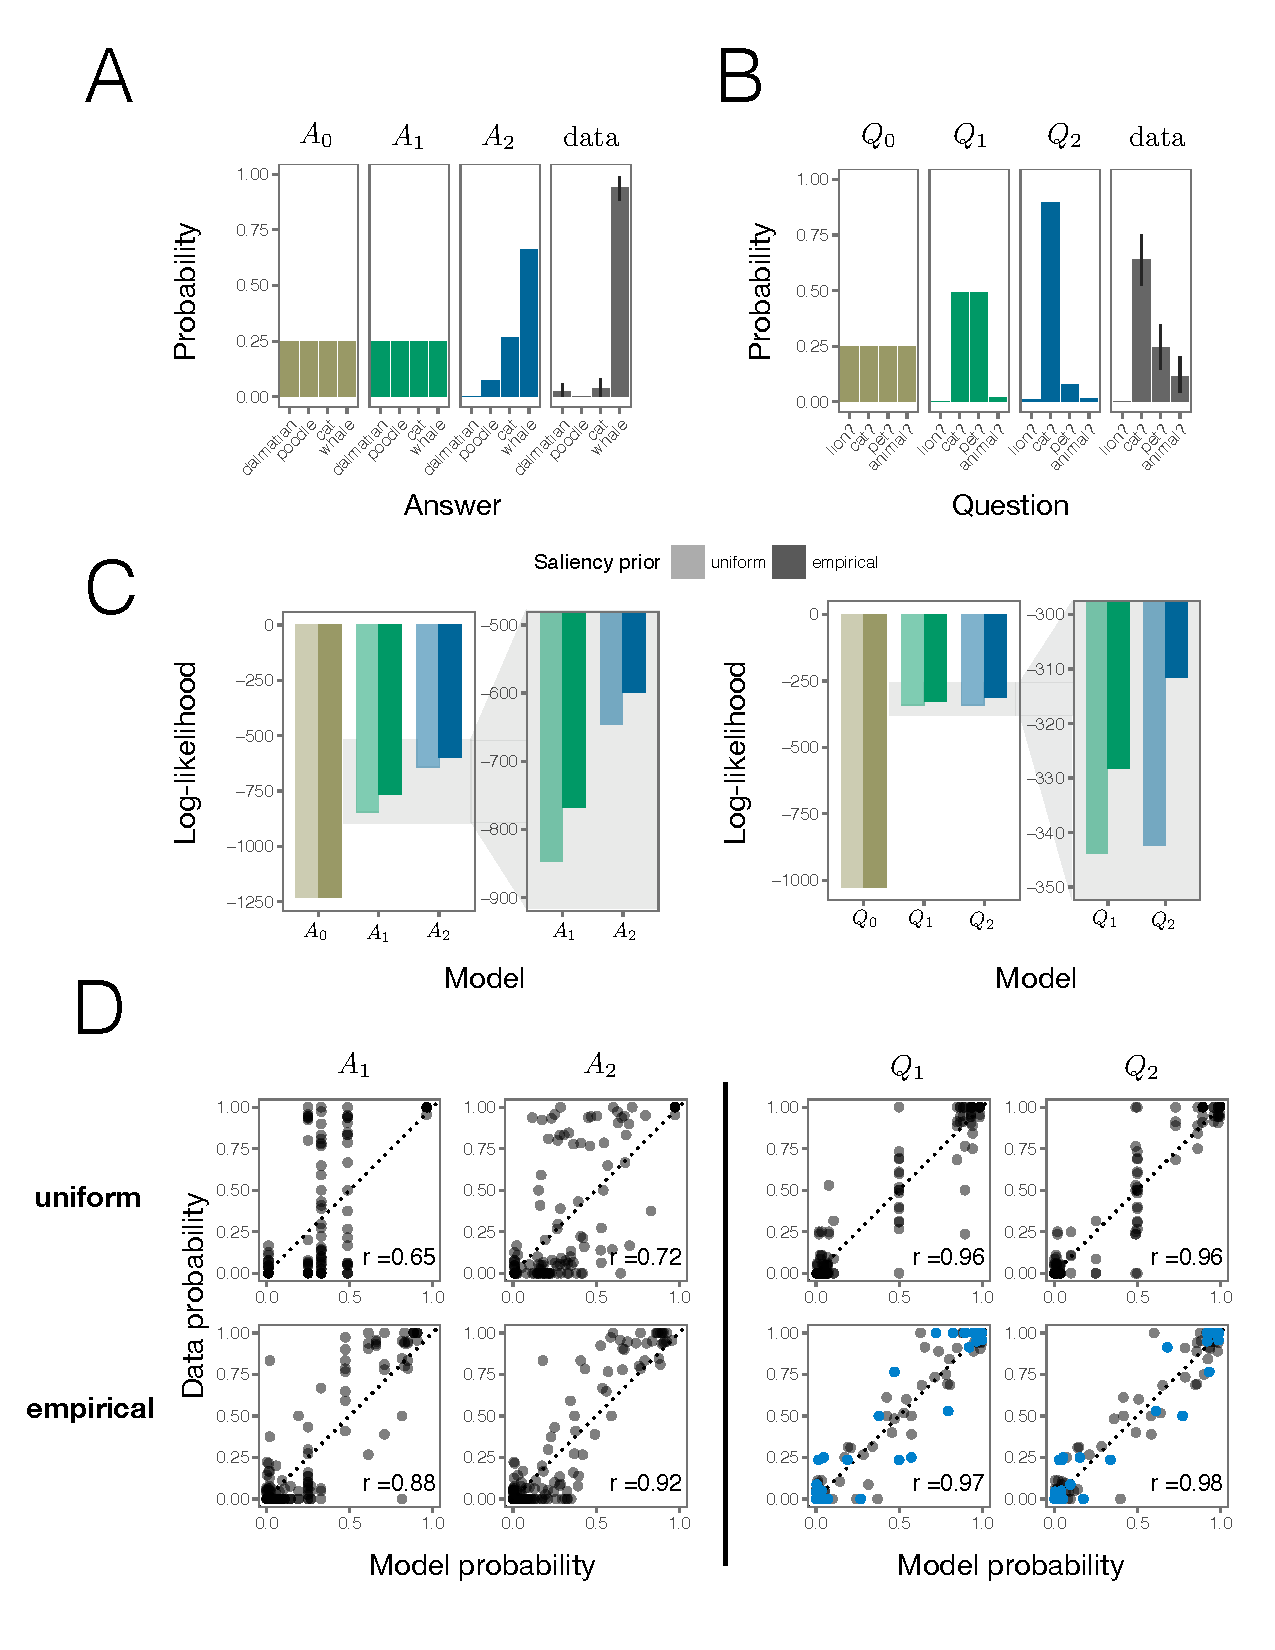
\includegraphics[scale = .77]{Exp1/ResultsFig.pdf}
\end{center}
\caption{Posterior predictives for each model (excluding $A_0$ and $Q_0$) given data from Experiment 1 compared to empirical data.}
%\vspace{-1cm}
\label{fig:exp1predictives}
\end{figure*}

%
%\begin{figure*}[t!]
%\begin{center}
%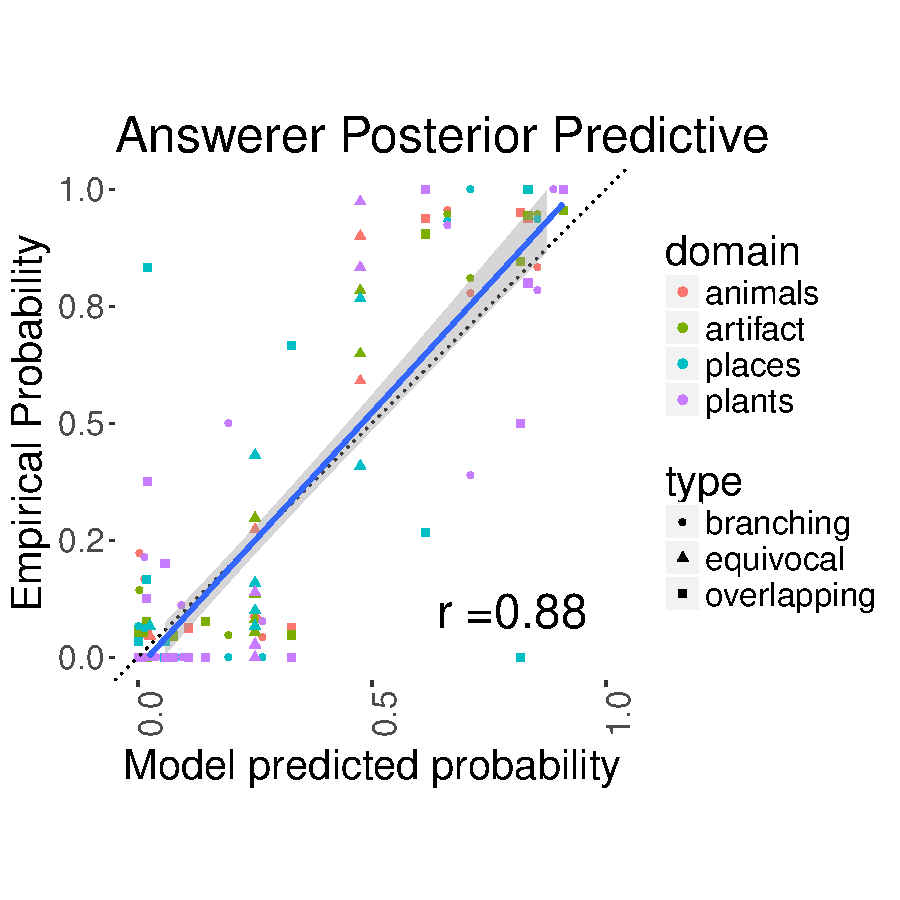
\includegraphics[scale=.5]{betaZeroAnswerer_Predictives}
%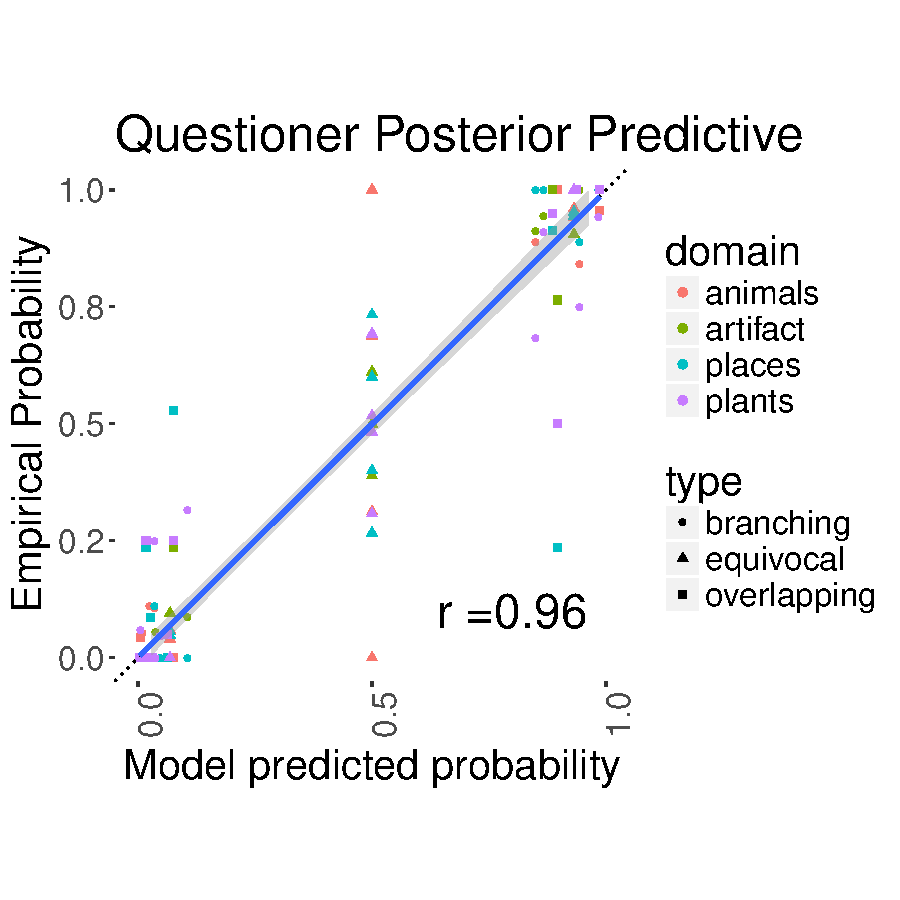
\includegraphics[scale=.5]{betaZeroQuestioner_Predictives}
%\end{center}
%\caption{Full space of models, and their correlations with the data, broken down by item and type.}
%\label{fig:answererPredictives}
%\end{figure*}


%

%

%\subsection{Discussion}

%%We also identified four shortcomings of Experiment 1. First, despite the success in distinguishing between answerer models, our data are not sufficient to distinguish between the explicit and pragmatic \emph{questioner} models. The two models did not make significantly different predictions for this experiment (and both are sufficient to account for the data). 
%
%
%

%First, we found additional evidence that $A_2$ answerer can account for essential qualitative features of the response data. For example, the explicit answerer predicts a uniform distribution over responses to the `animal?' question in the branching hierarchy. All four of the objects are animals and under the assumption that all four are equally salient, the question meaning projection is equally likely to pick out any of them. Contrary to these predictions, we found that answerers overwhelmingly preferred the response ``whale'' to the other three responses, which is accurately predicted by the Gricean dynamics of the pragmatic model. If the questioner were interested in any animal other than the whale, they would have asked a different question; since they didn't, they must have meant the whale. Like our final case study, this task required the answerer to use the questioner's utterance as a signal of their underlying goals.

%Additionally, we were able to test the predictions of the \emph{questioner} component of the model for the first time. We found that at an aggregate level, both $Q_1$ and $Q_2$ accurately predict what questions an agent will pick when faced with a particular goal. However, our results for the overlapping hierarchy in particular show that the pragmatic model is necessary to account for some critical aspects of the data. 

%% NOTE ABOUT OUTLIER, if necessary... 
%The ``place'' domain that we flagged as a potential outlier earlier in the results is the only domain that does not show the pattern of responses predicted by the pragmatic questioner model. This is likely due to the choice of images displayed to participants: the two ``parent'' nodes of the critical goal are ``bar'' and ``restaurant,'' and we represented the intersection of these two categories as a hotel lobby. However, the image we chose placed emphasis in the bar in the hotel, which likely biased participants toward the ``bar'' response instead of the ``restaurant response'' predicted by the pragmatic model. 

%Finally, we made certain assumptions in modeling our hierarchies, such as the assumption that participants do not consider whales to be pets despite the fact that it's technically possible. 

%We address these issues by collecting independent estimates of participants' saliency knowledge in interpreting definite articles. 
%We then recompute our model's predictions using empirical saliency priors, in place of our previous assumption of uniform saliency within a category. We conduct a new Bayesian data analysis using these new predictions to test (1) whether our models more appropriately capture item-level variability and (2) whether the pragmatic models still provides a better fit after controlling for typicality knowledge.

\subsection{Discussion}

%In three case studies, we first established that among our answerer models only $A_2$, which goes beyond the literal meaning of the question to infer and address underlying \emph{goals}, could account for classic qualitative answerer-sensitivity effects. 
In Exp.~1, we presented both answerer and questioner models with the  \emph{qualitative} and \emph{quantitative} challenge of accounting for trial-level variance in a Hidden Goal task. 
We found strong converging support for $A_2$ relative to our other answerer models and, for the first time, tested the predictions of our questioner models. 
While both $Q_1$ and $Q_2$ provided good predictive fits to our question-asking data, only $Q_2$ could account for asymmetries in the critical \emph{overlapping} condition and was therefore also preferred in a Bayesian model comparison. 
We also found that incorporating realistic identifiability priors to handle the definite article provided a substantially better fit to our data. 

There are two main reasons why it was important to incorporate these priors into our model.
First, failures to account for non-uniform factors like conceptual typicality could potentially invalidate the conclusions of our model comparison. 
For example, we expect a house cat to be a much more typical exemplar of the category `cat' than a lion. 
Hence, participants may not be choosing the house cat in this item for pragmatic reasons; they may just be expecting the definite description to identify the more typical member of the category. 
If this were the case, including common knowledge about typicality should improve the predictions of $A_1$ and $Q_1$, thus potentially `explaining away' any benefit of deeper pragmatics. 
After accounting for this potential confound, we still found strong evidence for $A_2$ and $Q_2$ over simpler models.

Second, without the empirical priors, $A_2$ and $Q_2$ fail to capture graded responses across different domains. 
This is especially striking in the `equivocal' condition where models using a uniform prior predict no preference in questioner behavior: if asking about the goldfish, which is both a ``pet'' and a ``fish,'' then the symmetry of the alternatives provides no reason to favor one label over the other. 
Instead, we found a high degree of variability across domains. 
For example, when questioners were trying to find a pet goldfish, 85\% of participants preferred the label `fish' to the label `pet,' even though both are technically true. 
In the `artifacts' domain, on the other hand, questioners had no preference between asking about the `seat' or `metal thing' when the objects (metal chairs) fell into both categories.

To understand how our elicited identifiability distribution helped to explain these data, consider that a Dalmatian is a far more typical and salient member of the `pet' category than a goldfish \cite{Rosch75}. 
Hence a questioner considering this knowledge as common ground would know that asking ``Where is the pet?'' would tend to elicit information about the Dalmatian, not the goldfish. 
If they were looking for information about the goldfish, they would then prefer to ask about the `fish' category, where a goldfish is a highly typical example. 
In these cases, we expect that typicality strongly guides interpretation of the embedded definite article in questions.

Our results in the overlapping condition also raise a broader question about depth of recursive reasoning in RSA models.
The predicted asymmetry between ``cat?'' and ``pet?'' that we used to qualitatively distinguish our $Q_1$ and $Q_2$ models is a \emph{second-order implicature}: it only emerges for models with chains of more than two embedded agents (i.e.~$Q_2$ but not $Q_1$).
Previous attempts to test such second-order implicatures outside the question-answer setting have found mixed evidence. 
For example, \citeA{franke2016reasoning} used a hierarchical analysis to conclude that only one participant (out of 50) was accurately described as a second-order speaker in an ad-hoc implicature task \cite<see also>{frank2017rational}.
We expect our data also represent a heterogeneous population of questioners and answerers, but it remains an open question for future work to investigate which aspects of the task facilitated this higher incidence of second-order inferences.
One hypothesis is that the use of natural images and familiar conceptual relationships removed certain cognitive demands imposed by the \emph{ad hoc} binary properties used in prior reference games.
A different possibility is that second-order reasoning is commonly needed for asking questions (but not for implicatures) and thus average language users exhibit this competence more in the question-answer setting.

Our model for Exp.~1 also served as a first demonstration of the ``composability'' of our computational framework with other formal proposals in linguistics and cognitive science.
Our model framework derives question and answer pragmatics from choices about literal question and answer semantics, world states, and goals. This allowed us to neatly accommodate definite reference and typicality effects in questions by importing proposals about definiteness developed in linguistics and philosophy.
In other words, the core computational framework itself did not need to be extended, only applied to the appropriate space of questions. 
In Exp.~2, we design a more targeted experiment to test our pragmatic questioner $Q_2$ and show that our model can similarly accommodate more structured \emph{goals}.

\section{Experiment 2: Structured goals}
\begin{figure*}[th!]
\begin{center}
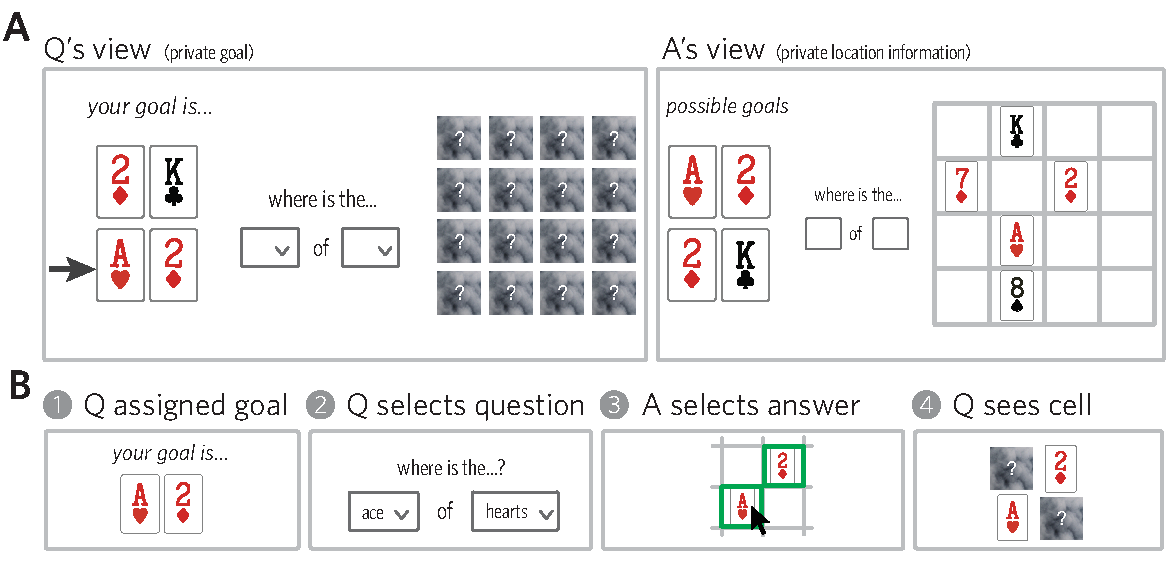
\includegraphics[scale = .9]{Exp2/task.pdf}
\end{center}
\caption{(A) Task displays and (B) procedure for Experiment 2. \ndg{in A can't tell that goal sets are grouped by rows (was this clear in expt?). maybe add a separating line or a little more space?}}
%\vspace{-1cm}
\label{fig:exp2task}
\end{figure*}

The construct of a goal has a long history in psychology \cite{miller1960plans, Schank:1977hh, austin1996goal}.
The simplest spaces of goals, like those used in Exp.~1, are discrete sets of projections on the world state.
For example, in the Stroop task commonly used to study cognitive mechanisms of goal-directed behavior, the goal is either to (1) read the presented word or (2) name the color in which they are written \cite{miller2001integrative}.
However, for more complex behaviors, it is often useful to represent goals in \emph{hierarchically structured} spaces \cite{badre2008cognitive,botvinick2008hierarchical}: we often need to achieve multiple subgoals in pursuit of a larger, more abstract goal. 
These more structured representations have also been key to explaining third-party goal inferences in Bayesian models of theory of mind \cite{BakerSaxeTenenbaum09_ActionUnderstandingInversePlanning}. 
For example, if we know an agent takes the same route home every day, but one day we observe them veering off of this route toward the grocery store, we simply infer that they intend to run this errand as a subgoal of their ultimate goal of getting home. 

The hierarchical structure of goals has also long been recognized in linguistic theories of questions in discourse  \cite{Kuppevelt95_TopicalityDiscourse,Roberts96_InformationStructureDiscourse,Buring03_DtreesBeansBaccents,Groenendijk99_LogicOfInterrogation,rojas2014discourse}.
For instance, if a traveler asks \emph{Are there window seat tickets to Berlin at 7:00?} and there are no such tickets available, it would be more helpful for the travel agent to respond \emph{the next available tickets are for 10:00} than \emph{no} \cite{rojas2013roadsigns}.
This has been understood as a recognition by the agent that the specific flight and seat preference mentioned by the traveler are subgoals in a hierarchy below the broader goal of getting to Berlin. 

Structured goals of this type are naturally accommodated by our framework. 
To show this, we designed a simple Hidden Goal collection game inspired by recent experiments in multi-task reinforcement learning \cite{oh2017zero, andreas2017modular}.
Furthermore, this task provides an additional, stronger test of the pragmatic questioner model $Q_2$.


As in Exp.~1, participants were either assigned the role of questioner or answerer, the questioner was given a private goal, and the answerer was given private information that was necessary for the questioner to fulfill this goal.
Unlike Exp.~1, however, each goal was a \emph{combination} of multiple objects that must be collected rather than a single object.
More specifically, the questioner was privately assigned a hand of playing cards to find (Fig. \ref{fig:exp2task}A, left). 
The cards were scattered around a grid, and only the answerer had visibility of where the cards were located (Fig. \ref{fig:exp2task}A, right).
The possible hands of cards the questioner might be assigned to collect were shared in common ground.

These multi-object goals induce a hierarchy where the ultimate goal of collecting the full set was decomposed into subgoals of finding each individual object in the set.
A pragmatic answerer, then, ought to infer and relevantly respond not only to the questioner's current subgoal but also their likely ultimate goal.
A pragmatic questioner, in turn, ought to be sensitive to which questions best signal the ultimate goal, beyond any particular subgoal.


\subsection{Methods}
\subsubsection{Participants}

We recruited 62 participants from Amazon Mechanical Turk to play a communication game.
We excluded 4 participants who disconnected before completion, 10 participants who failed pre-specified catch trials (see below), and 3 additional participants who self-reported confusion about the instructions.
This left 45 participants in our final sample, each of whom provided responses in both the questioner role and the answerer role.

\subsubsection{Stimuli}

Stimuli were constructed from a standard deck of 52 playing cards (4 suits $\times$ 13 ranks). 
For each trial, we randomly sampled between 5 and 9 cards from the desk. 
These cards were randomly assigned to locations in the grid. 

We constructed the space of goal ``combos'' on each trial in two different ways, leading to two conditions where our questioner models made qualitatively different predictions.
In the \emph{baseline} condition, we sampled two disjoint sets containing two cards each. 
In this case, both models predict that the questioner should have no preference over which card to ask about.
In the \emph{overlapping} condition, we again sampled two sets containing two cards each but ensured that one card appears in both sets. 
Here, our pragmatic model predicts that the questioner will avoid asking about this card; although it is a necessary subgoal, it would provide an ambiguous signal to a pragmatic answerer about the ultimate goal.

Finally, we constructed catch trials using single-object goals. 
Because there is only one card that must be found to complete the hand, questioners ought to ask about this card and answerers hearing this question ought to (at least) reveal the requested card.
If the questioner asked about a different card, or the answerer failed to reveal the card that was asked about, we took this as a grounds for exclusion due to inattentiveness.

\subsubsection{Procedure}

Each trial proceeded through the same four phases as Exp.~1. 
Questioners were first assigned a ``combo'' to complete out of a shared list of possible alternatives and used dropdown menus to choose a suit and rank to ask about (e.g. ``Where is the king of hearts?'').
Upon seeing this question, the answerer selected either one or two cards to reveal to the questioner and the questioner was then shown the locations of these cards.

If all of the cards in their combo were revealed, participants advanced to the next trial; if not, the questioner was prompted to try again.
It was always possible to complete the combo in a single exchange.
To incentivize performance, we gave a bonus when the exact cards in the combo were revealed on their first try. 

The trial sequence was constructed such that each participant saw each of the three trial types (baseline, overlapping, and catch trials) once as questioner and once as answerer for a total of six trials.
We grouped trials into two blocks, one for each role, with the sequence of conditions randomized within each block.
The starting role was counterbalanced across participants.

Unlike Exp.~1, which used a real-time multi-player methodology to ensure participants knew they were playing with a real partner, we decided in this experiment that the benefit of such minimal interaction was not worth the loss in control over the input given to participants.
Instead, participants were paired with an artificial agent that played the opposite role.
When in the questioner role, this agent selected question stimulus with maximum probability according to $Q_2$. 
This choice ensured that we densely sampled answer responses in the cases where the answerer models made diverging predictions.
In the answerer role, the artificial agent similarly responded according to $A_2$, which was intended to minimize participant frustration.

Using our models directly in the task admittedly presents a potential for `contamination' where participants imitate or learn from the model's behavior. 
We addressed this concern in two ways. 
First, the experiment is limited to only six trials, minimizing the potential for learning.
Second, because we counterbalanced the order in which roles were assigned, we will empirically test whether patterns of responses differed for participants who had already seen their partner respond in a role.

\subsection{Predictions and results}

\subsubsection{Model setup}

\ndg{let's discuss the math in this section...}

Exp.~2 was designed to provide a strong \emph{qualitative} test of the questioner models in a scenario with more structured goals.
We formalize the notion of a goal hierarchy by extending the goal space $\mathcal{G}$ from a set of possible goal projections $\{g_i\}$ to a set of ordered pairs $\{g_{ij}\} = \{(g_i, g_i^{(j)})\}$ where $g_i$ represents an ultimate goal and $g_i^{(j)}$ represents a subgoal of $g_i$. 
In the case of Exp.~2, $g_i$ represents the goal of finding an entire combo $i$ --- the projection from the world $w$ to the list of locations of all cards in the combo --- while $g_i^{(j)}$ represents the simpler goal of finding just the single $j$th card in the $i$th combo. 


\begin{figure*}[th!]
\begin{center}
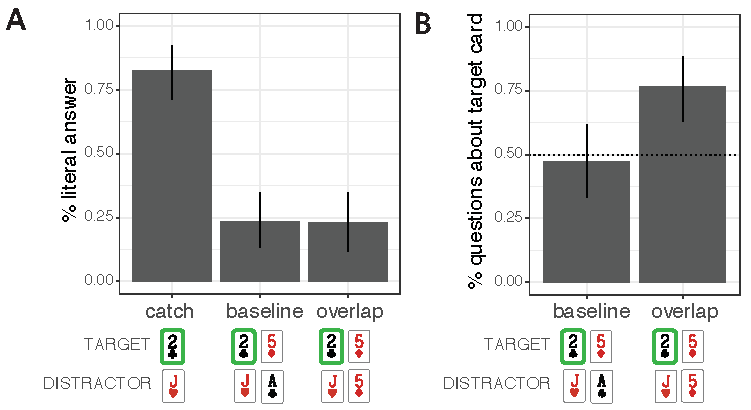
\includegraphics[scale = 1]{Exp2/qualitativeResults.pdf}
\end{center}
\caption{Results for Exp.~2. (A) Answerers are more likely to go beyond the literal question and reveal additional cards in the baseline and overlap conditions. (B) Questioners are more likely to ask about the non-overlapping card relative to baseline. Dotted line is chance, and error bars are bootstrapped 95\% CIs.}
%\vspace{-1cm}
\label{fig:exp2results}
\end{figure*}

The primary computational consequences of introducing a hierarchical goal space emerge from the pragmatic answerer $A_2$. 
Upon hearing a question, $A_2$ must jointly infer the ultimate goal along with the current subgoal.
First, we assume that a questioner acting under an ordered pair $g_{ij} = (g_i, g_i^{(j)})$ attempts to gain information towards both goals:
$$P_{Q}(q | g_{ij}) = \prod_{g\in \{g_i, g_i^{(j)}\}} P(q | g)$$
\ndg{this is not normalized. is this actually what's implemented? it's a kind of strange assumption compared to eg adding the utilities of the two sub-goals (which is different because of normalization).}
In other words, a question is preferred if it is both good for the current subgoal and the ultimate goal.
% of finding the entire privately assigned combo $i$.
Combining this assumption about the questioner $Q_1$ with the dependence between subgoal and ultimate goal, $A_2$'s goal inference factors as:
$$\begin{array}{rcl}
P(g_{ij} | q) & \propto & P(q | g_{ij})P(g_{ij}) \\
 & = & P(q | g_i)P(g_i) \cdot P(q | g_i^{(j)}) P(g_i^{(j)} | g_i)
 \end{array}$$
Given a posterior over the goal tuple $g_{ij}$, we then assume the answerer attempts to be informative with respect to both goals in the tuple: 
$$U_{A_2}(a; q, w) = \sum_{g_{ij} \in \mathcal{G}} P(g_{ij}|q) \sum_{g\in \{g_i, g_i^{(j)}\}}\widehat{P^g_I}(w|\,a)$$
 \ndg{hmm is there a clearer way to describe this? does it follow from the tuple projection? also, missing log}
While this presentation was written in terms of ordered pairs, it straightforwardly extends to deeper goal hierarchies represented as $n$-tuples. 
The simpler goal spaces considered earlier in the paper are special cases of this more general formulation taking goal tuples to be singletons.

Given this generalization of the model to more structured goal spaces, we can derive predictions for Exp.~2. 
The world space $\mathcal{W}$ consisted of all assignments of cards to locations.
Questions in the question space $\mathcal{Q}$ were of the same form as in Exp.~1 (``Where is the X?''), but because X was always constrained to be a unique card, issues of multiple identifiability do not arise. 
Finally, the answer space $\mathcal{A}$ consisted of any combination of one or two card locations, which evaluate to true in worlds where the card or cards are in fact at the location that was mentioned, and false otherwise.



\subsubsection{Answerer results}

Although the different conditions of the experiment were primarily designed as a stronger qualitative test of the questioner model, it also provides another opportunity to test the answerer models. 
To begin, consider the simple catch trials, where each goal contained only one card.
Here, both $A_1$ and $A_2$ make the same prediction: that participants will reveal the single card that was asked about with high probability and, with lower probability, they may be ``overinformative'' by revealing both the card that was asked about along with some other card.
Indeed, we found that 83\% of participants responded literally with the exact card asked about, while the remaining 17\% gave overinformative responses (Fig. \ref{fig:exp2results}A).
The precise probability the models put on such overinformative responses depends on the optimality parameter $\alpha$ and a cost parameter penalizing longer answers; at a cost penalty of $1$, the empirical response distribution is obtained with moderate values of $\alpha=3$ for $A_2$ and $\alpha = 3.5$ for $A_1$.

In the \emph{baseline} and \emph{overlapping} conditions, however, $A_1$ and $A_2$ make diverging predictions. 
$A_1$ treats these conditions the same as the catch trial, since it attempts to be directly informative with respect to the goal inherent in the question, and all questions are about a single card.
$A_2$, on the other hand, goes beyond the literal question to infer that the questioner asked about just one subgoal of one of the ultimate goals.
When asked about a card that appears in one goal combo but not the other, $A_2$ infers with high probability which of the two ultimate goals is most likely the hidden goal. 
It is thus much more likely to respond with \emph{both cards} than about only the single card that was asked about (or any other combination of cards). 
We found that only 23\% of participants gave literal answers in each of these conditions, which is significantly different than the proportion (83\%) in catch trials, $\chi^2(1) = 35, p < 0.001$, Fig. \ref{fig:exp2results}A.
The empirical response distributions for these conditions are thus consistent with the predictions of $A_2$ and strongly falsify $A_1$.

\subsubsection{Questioner results}

Next, we turn to questioner behavior, the primary focus of Exp.~2.
The $Q_1$ and $Q_2$ models make qualitatively different predictions about which questions participants chose in the \emph{overlap} and \emph{baseline} conditions.
$Q_1$ predicts no difference in behavior across these two conditions.
Because it reasons that $A_1$ will always provide a literal or (indiscriminately) overinformative response, as we saw in the previous section, then asking about either card is equally useful for completing the target combo.

The pragmatic questioner $Q_2$, on the other hand, recognizes that certain questions may provide better signals about the ultimate goal than others.
In particular, for the \emph{overlap} condition, $Q_2$ reasons that if they asked about the card appearing in both combos, $A_2$ would not be able to infer which of the two combos is their ultimate goal.
If they instead asked about the unique card, however, $A_2$ would infer their true goal with high probability and subsequently be more likely to reveal the needed information.
Thus, $Q_2$ predicts that participants will prefer to ask about the unique card.
The \emph{baseline} condition serves as a control where both cards are unique, hence both questioner models predict no preference over the two cards.

We found that 77\% of participants asked about the unique card in the overlap condition, which is significantly different from the null probability of 50\% predicted by $Q_1$, $\chi^2(1) = 11.3, p < 0.001$. 
Meanwhile, the proportion of participants (48\%) who asked about the card in the same position in baseline trials did not differ from chance: the Bayes Factor for binomial proportions  \cite{morey2016philosophy, morey2015package} shows weak evidence in favor of the null, $BF = 0.37$, Fig. \ref{fig:exp2results}B. 
This qualitative pattern of responses is consistent with the predictions of $Q_2$ but cannot be explained by $Q_1$.

It was possible, however, that this pattern was driven by participants who had already seen their partner ask about the unique card on a previous trial and were copying their behavior. 
To address this concern, we examined these response patterns for the subset of participants who were assigned the role of the questioner on the first half of trials and thus had no opportunity to learn from their partner: 18 of these 21 participants (87\%) asked about the unique card, which remained significantly different from chance: $\chi^2(1) = 9.3, p = 0.002$.

\subsection{Discussion}

Exp.~2 was motivated by two primary aims: to provide a stronger evaluation for the questioner models, and to demonstrate how our core framework generalizes to more structured spaces of goals.
To meet these challenges, we designed a Hidden Goal task where questioners were privately assigned a set of \emph{multiple} objects to find, inducing a hierarchy of subgoals.
By manipulating whether objects overlapped or differed across sets in the space of possible goals, we constructed scenarios where our different models made sharply different predictions. 

\ndg{somewhere should indicate why the obvious application of the model, where goals are just the location of the complete set, doesn't work.}

We found that answerers reasoned beyond the literal subgoal prompted by the question to respond helpfully to the inferred ultimate goal in the hierarchy.
Questioners, in turn, chose to ask about the objects that would most clearly signal their ultimate goal to their partner, even though these different questions would have equal expected information gain under traditional models. 

\ndg{let's condense the next three paragraphs? they are kind of wordy and aside...}

The minimal goal hierarchy studied in Exp.~2 is a key first step toward formally addressing more structured spaces of goals in cognitive models of question asking and answering. 
However, handling more complex goal structures will require composing our core computational framework with additional mechanisms.
In particular, we relied on the simplifying assumption of different subgoals being \emph{conditionally independent} given their parent in the hierarchy. 
This assumption justified the representation of subgoals as ordered pairs with their parent, as well as the decomposition of the utility such that each subgoal equally contributes to the ultimate goal. 

This assumption is clearly violated in certain real-world cases.
For example, the overarching goal of making coffee decomposes into subgoals of turning on the faucet, boiling water, grinding beans, and so on \cite{jackendoff2007language}. 
These subgoals unfold in time, introducing sequential dependencies.
If we are trying to make coffee in an unfamiliar kitchen, certain questions may only be useful once earlier subgoals have been satisfied, leading to more or less optimal sequences of questions.
Conversely, answerers may take advantage of schematic knowledge of this sequential structure to anticipate subsequent subgoals: if a questioner asks ``Where do you keep your coffee beans?'', they are likely earlier in the process than if they asked ``Do you have a mug?'' 

Deciding how to ask and answer questions in the presence of such sequential dependences in the goal space likely requires a \emph{planning} mechanism over a persistent state.
Planning may also be necessary for integrating the pragmatics of question asking and answering into longer dialogue sequences, as it has been for other domains \cite<e.g.>{bramley2015conservative}.
While introducing such a planning mechanism into our model is outside the scope of this paper\footnote{The optimality of asking questions based on global planning policies, compared to locally `greedy' policies, is not yet well-understood even in the non-social case of querying an oracle, though see \cite{nelson_meder_jones_2018} for recent theoretical progress.}, our final experiment aims to set a foundation for future work by (1) introducing a notion of persistent state into the model and (2) investigating several pragmatic phenomena that emerge from iterating our model forward in time in a step-wise manner.
%In the next section, we set the foundation for future work on more extended dialogue by investigating certain features of multi-round dialogue that do not require planning.

\section{Experiment 3: Extended dialogue}

In our computational framework, an answerer updates their beliefs about the questioner's goals after hearing a question, and a questioner updates their beliefs about the world state after hearing an answer. 
In principle, this step can be repeated multiple times until the questioner's goal is resolved, allowing for an extended sequence of questions and answers: the questioner's posterior over worlds after hearing an answer to their first question becomes the prior for selecting their second, and so on.

\ndg{somewhere (maybe earlier or maybe discussion for this section) should mention khani etal, and indicate some differences.}

In Exp.~3, we developed a final task in the Hidden Goal paradigm to investigate how the pragmatics of asking and answering questions unfolded over multiple exchanges.
This task was designed with several desiderata in mind.
First, we needed a larger and more natural space of goals that wouldn't always possible to satisfy in a single round.
This would allow us to test our models' predictions about how the answer to one question may influence the choice of a subsequent question, or how the answerer's beliefs about the questioner's goal may shift after hearing additional questions.
Second, although $A_2$'s internal goal inference mechanism was implicit in the success of our model predictions in Exps.~1 and 2, we sought explicit validation of this model component by directly eliciting answerers' beliefs about the questioner's goal.

\begin{figure*}[tbh!]
\begin{center}
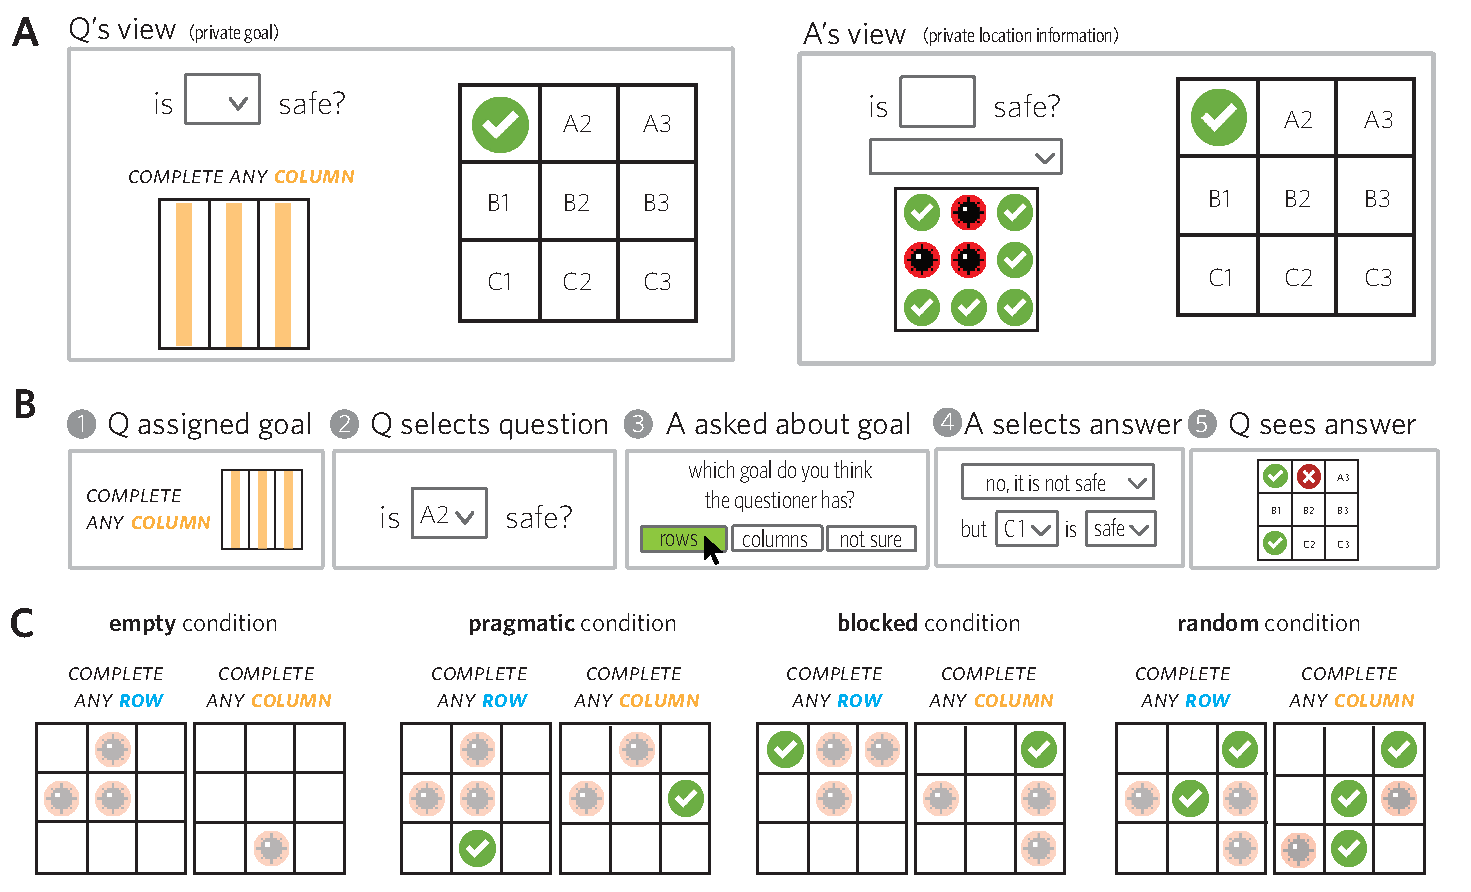
\includegraphics[scale = .7]{Exp3/spatialDemo.pdf}
\end{center}
\caption{(A-B) Task design and procedure for Experiment 3. Answerers are shown a private map with bomb locations, while questioners are assigned a private goal. Both participants see a common board over which extended dialogues can take place. (C) Examples of initial board states in different conditions. \ndg{maybe indicate in B that this then repeats?}}
%\vspace{-1cm}
\label{fig:exp3task}
\end{figure*}

The \emph{Don't Explode} task is a cooperative communication game inspired by Battleship and Minesweeper (see Fig. \ref{fig:exp3task}). 
Participants are presented with a shared $3 \times 3$ grid and told that some tiles are safe but others contain bombs.
One player---the questioner---is privately assigned a particular goal pattern they must complete by revealing tiles.
The other player---the answerer---is given a map showing where the bombs are.
As in our previous experiments in this paradigm, the answerer has uncertainty about the questioner's goal, and the questioner has uncertainty about the map.
To succeed, then, the questioner must ask questions (e.g. \emph{Is tile X safe?}) and the answerer choose what information to reveal in response.

\subsection{Methods}

\subsubsection{Participants}

We recruited 124 participants from Amazon Mechanical Turk, 21 of whom were excluded for disconnecting before the end of the task. 
This left 104 participants in our final sample, yielding a dataset of 1774 question trials and 1801 answer trials. 
All participants were self-reported native English speakers.

\subsubsection{Stimuli}

Each trial was defined by three stimulus choices: (1) a choice of goal, (2) an underlying `map' assigning bombs to locations, and (3) an `initial state' indicating which tiles were shown as safe to both players at the outset of the trial.
By manipulating the state of the initial grid, we generated a large number of items where our models make different predictions. 

Goals were sampled from a space of two ultimate objectives: complete any \emph{row} or complete any \emph{column} (see Fig. \ref{fig:exp3task}A).
Because these goals are logical disjunctions, they could be satisfied in as many ways as there are rows or columns, inducing a hierarchical goal space with each row/column as a possible subgoal the questioner could pursue.
This goal space was intended to be intuitive for participants, given its resemblance to the win conditions of well-known games like Tic-Tac-Toe or Connect Four.

Underlying bomb maps were sampled from the space of all assignments of bombs to locations,  subject to the constraint that it was possible to win given either goal. 
We included this constraint so that the arrangement of bombs did not give the answerer any cues to the questioner's goal.
Finally, the initial state of the shared board was chosen from four different conditions to create a variety of different scenarios (see Fig. \ref{fig:exp3task}C for examples).
Cells in the shared board were labeled with coordinates (A1, A2, $\dots$ ) for easy reference.
\begin{itemize}
\item In the \emph{empty} condition, no tiles were included in the initial state.
\item In the \emph{pragmatic} condition, a single tile was included in the initial state. This tile was chosen from a completely safe row or column, depending on the goal.%, such that asking another question in that row or column would provide a clear signal of the goal and allow the answerer to complete the goal after a single question.
\item The \emph{blocked} condition was similar to the pragmatic condition, except a bomb was placed in the row or column partially completed by the initially revealed cell. %This set the grounds for a scenario where questioners may have to adjust their subgoal upon hearing a response.
\item The \emph{random} condition randomly sampled a subset of safe tiles from the map, under the constraint that they did not fully complete a row or column. 
\end{itemize}

\subsubsection{Procedure}

The task procedure was adapted from that of Exps.~1 and 2 to support extended exchanges. 
First, questioners were shown their assigned goal and selected a cell label from a dropdown menu to ask a question of the form ``Is X safe?''. 
Answerers selected a yes/no answer to this question and were presented with the option to either send more information or to continue with only this yes/no answer.
If they chose to send more information, we showed dropdown menus with all possible cells, allowing for responses like ``no, X is not safe, but Y is.''
Finally, this answer was shown to the questioner.
If the new information fulfilled the goal, participants advanced to the next trial.
If the goal was not fulfilled, the questioner was prompted to ask another question, and the cycle repeated.
Participants received a bonus on each trial related to the number of exchanges taken before completing the goal: one cent was subtracted from a total of \$0.05 for each additional question.%, down to a minimum of \$0.00.

We elicited the answerer's beliefs about the hidden goal after they saw the questioner's message but before they made their response.
Three response options (``rows,'' ``columns,'' or ``not sure'') were provided to the prompt ``Which goal do you think your partner has?'' 
No feedback was provided for this response.
For the other responses, answerers were prevented from sending blatantly false information (e.g. saying there was a bomb when there was no bomb), and questioners were prevented from asking about tiles that had already been revealed.

Participants alternated between the roles of questioner and answerer for a sequence of 20 trials. 
To acquaint participants how the task worked, all trial sequences began with two practice trials, followed by four random trials.
Practice trials were constructed by including two of the three cells of a goal-relevant column or row in the initial state. 
It should have been clear from a basic understanding of the instructions that the questioner needed to ask about the third cell and the answerer ought to reveal it. 
After these initial six trials, we constructed a scrambled sequence where each condition appeared once in each role and these critical trials were interspersed with more random trials.
As in Exp.~2, participants were paired with an artificial agent playing the opposite role. 
This agent acted according to our $Q_2$ and $A_2$ models, with the optimality parameter set high ($\alpha = 100$). 

\subsection{Results}

\subsubsection{Model setup}

The key innovation required to account for extended sequences is an explicit representation $s_t$ of the \emph{discourse state} at a given time. 
In general, the discourse state could contain prior utterances and any non-linguistic observations about the agent's partner or context.
In this experiment all information was updated and maintained visually, so it is sufficient to take as $s_t$ the literal state of the game board shared in common ground at time $t$.

Each state is then associated with a conditional belief distribution over the world, $P(w | s_t)$.\footnote{This notion of a belief state can in principle be used to define a Markov Decision Process, where different question or answer selections lead to anticipated transitions in beliefs. This connection suggests a future avenue toward embedding our pragmatic agents in a planning framework. \ndg{move this comment to discussion, connect to khani etal}}
In our experiment, computing this distribution simply entailed removing any world states from the prior that are incompatible with the current revealed state and re-normalizing.
Now, when a questioner is selecting a question in state $s_t$, rather than taking expected information gain relative to the initial prior $P(w)$, they use their current beliefs $P(w | s_t)$ as the baseline.
Moreover, since the discourse state $s_t$ is in common ground, we assume this alternative prior is used throughout internal levels of recursion, e.g. that $A_1$ also attempts to be informative with respect to this prior.

Beyond introducing state to handle extended exchanges, the task details for this experiment were formalized similarly to the previous experiments.
The world prior was uniform across all $2^9$ assignments of bombs to tiles. 
The question space contained the 9 options available to participants in the experiment, where ``Is A1 safe?'' is represented as a projection from the full world to the status of the queried tile. 
The answer space contained both the literal answers ``yes, it is safe'' and ``no, it is not safe,'' as well as longer answers that additionally mentioned the state of another tile, e.g. ``yes, it is safe but A3 is not.''

Goals were again represented hierarchically, with a joint representation containing rows vs.~columns at the super-ordinate level and \emph{which} row or column at the subordinate level.
The super-ordinate row (column) goals projected worlds to arrays of three booleans representing which rows (columns) contained bombs and which did not.
The subgoal representing a particular row (column) projected worlds to a single boolean representing whether that particular row (column) contained bombs.

\subsubsection{Hidden goal inferences}


\begin{figure}[t!]
\begin{center}
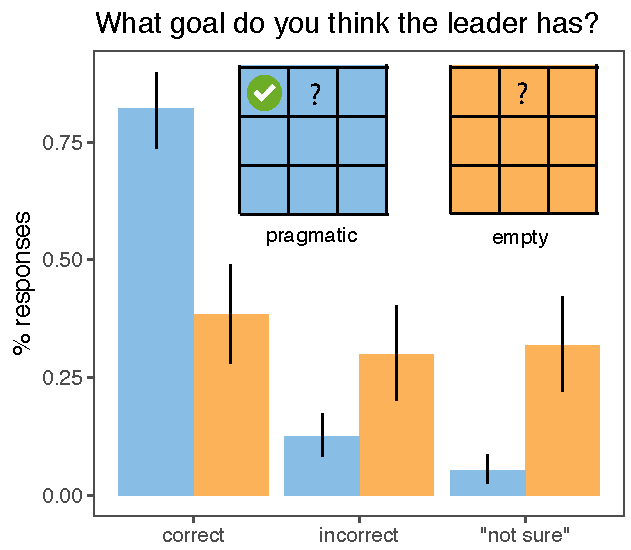
\includegraphics[scale = .8]{Exp3/spatialGoalInference_final.pdf}
\end{center}
\caption{Goal inferences shift with additional questions. Curves are the proportions of empirical answerer responses to ``Which goal do you think your partner has?''  after hearing the $k$th question. Error ribbons are bootstrapped 95\% CIs.}
%\vspace{-1cm}
\label{fig:exp3goalinference}
\end{figure}


\begin{figure*}[t!]
\begin{center}
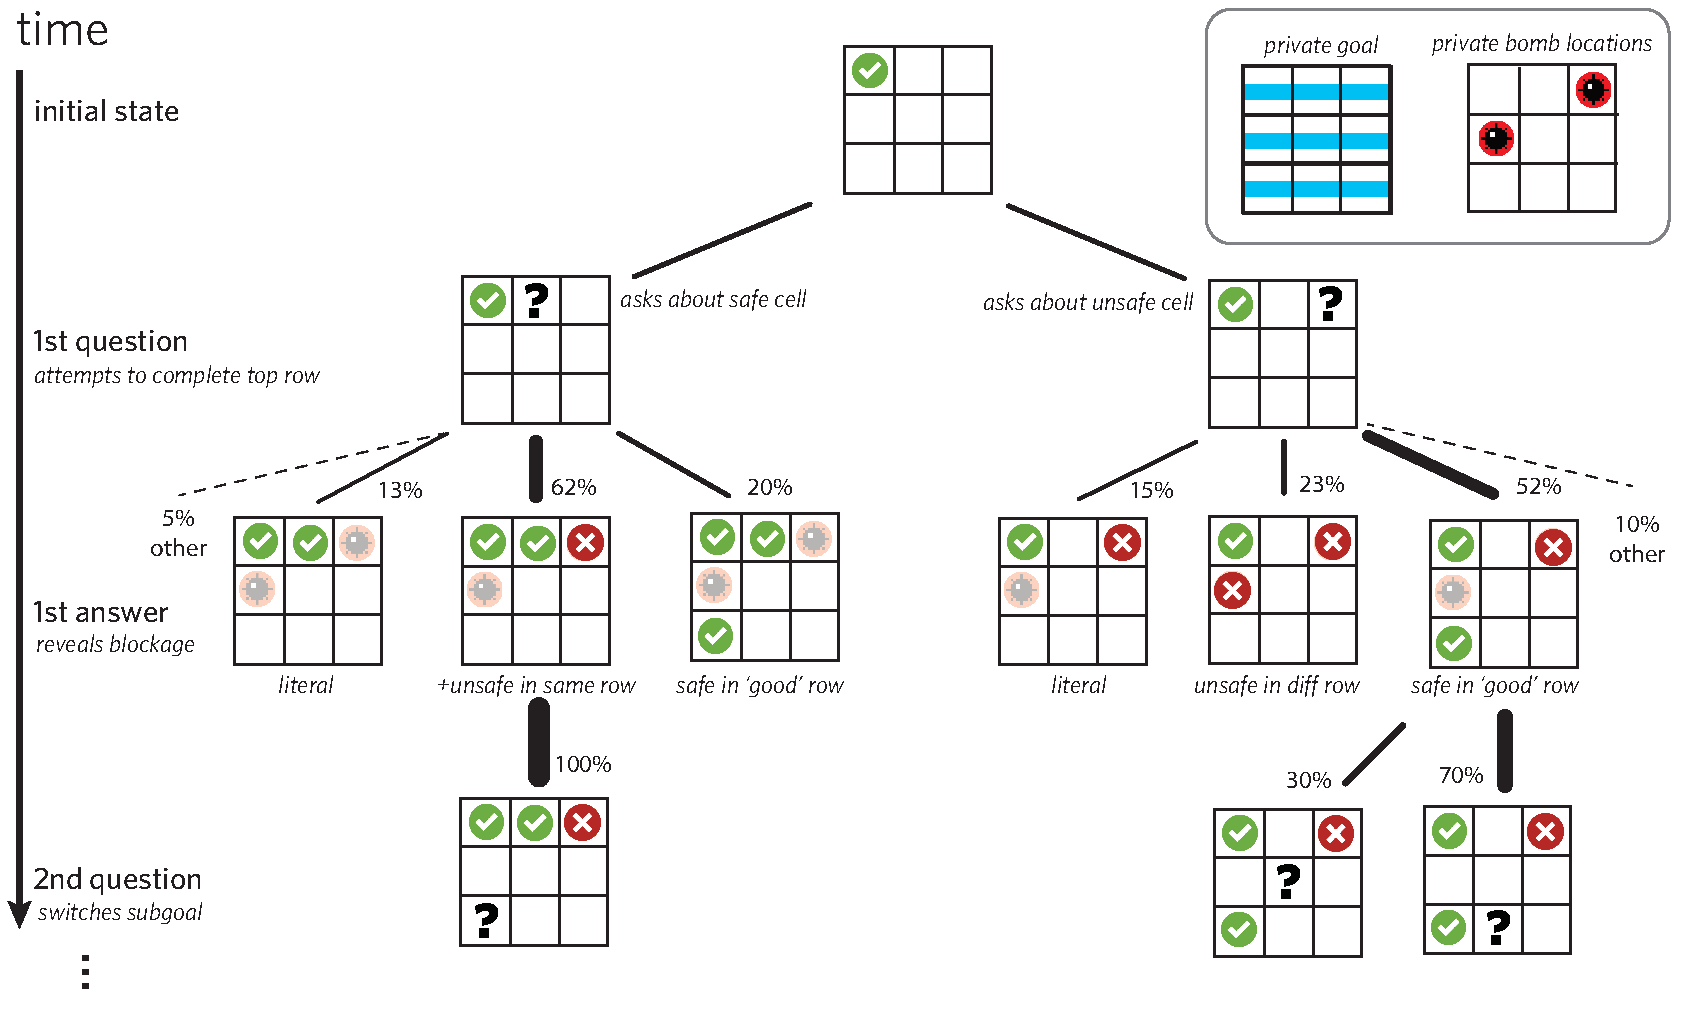
\includegraphics[scale = .6]{Exp3/blocked.pdf}
\end{center}
\caption{Decision tree of questions and answers in `blocked' condition as dialogue unfolds. Response probabilities are empirical estimates; line width is proportional to response probability.}
%\vspace{-1cm}
\label{fig:blocked}
\end{figure*}


A primary internal mechanism driving pragmatic behavior in our models is $A_2$'s Bayesian inference about the questioner's goal conditioned on the question. 
While the overall success of $A_2$ in predicting answerer behavior in Exps.~1 and 2 provided indirect evidence for this mechanism, the elicitation step included in our design provides the opportunity for a more direct test of the answerer's beliefs about the goal.
Do participants' inferences about the questioner's true goal match those internally predicted by the model?

We examined participants' goal inferences in the \emph{empty} condition, which was designed to measure the changes in answerer's beliefs about the hidden goal over repeated exchanges. 
$A_2$ predicts that the first question should provide no information about the hidden goal: $Q_1$ is equally likely to ask about any cell under either goal.
In the context of the information revealed in the first exchange, however, the $A_2$ model predicts that the second question ought to license stronger inferences.
We compared these shifts in the empty condition against those in the \emph{pragmatic} condition, which served as a baseline.
In the pragmatic condition, the $A_2$ model predicts that sufficient context is already available from the initial state to make a strong goal inference.

We aggregated data across the two possible goals by classifying responses as `correct' if they matched the true goal and `incorrect' if they differed.
We found that after the first question in the ``empty'' condition, participants were roughly at chance between the response options, only guessing the true goal with 39\% accuracy\footnote{Apparently some proportion of participants simply guessed instead of using the ``not sure'' option, which received 31\% of responses.}.
After the second question, however, they were able to infer the true goal with 82\% accuracy (see Fig. \ref{fig:exp3goalinference}).
The distribution over the response variables changed significantly from the first to second question, $\chi^2(2) = 31, p < 0.001$.

Furthermore, answerers' goal inferences after the second question in the empty condition were close to those observed after the \emph{first} question in the baseline pragmatic condition (82\%), where we initialized participants with similar information in common ground.
These results provide a direct validation of the internal mechanism of goal inference.
Answerers systematically use context to make accurate inferences about their partner's goals, whether that context is provided in the initial common ground or by earlier question-answer exchanges.

\subsubsection{Questioner behavior across multiple exchanges}

Just as the answerer's beliefs about the hidden goal shifted with each question, the questioner's beliefs about the world ought to shift with each answer. 
In particular, this shifting belief state provides a mechanism for the answer to one question to affect the selection of a follow-up question.
%In particular, shifting beliefs about the world should  questioners may prefer different follow-up questions depending on the answer to their first question, 
%To evaluate this prediction, we consider how dialogue unfolded in the \emph{blocked} condition.
The \emph{blocked} condition was designed precisely to empirically elicit such sequences, providing a key test of our model's ability to handle the updating state.
In this condition, questioners are faced with a setback: there was a hidden bomb in the row or column that would provide the shortest path to goal completion.
Answerers in this condition therefore needed to decide how to most helpfully reveal this setback, while questioners needed to decide how to use this initial answer to proceed in future exchanges.

In Fig. \ref{fig:blocked}, we show a schematic view of how dialogue unfolded in an example blocked trial.
Given the initial common ground that the top-left tile was safe, and their private goal to complete any row, questioners began by either asking about A2 or A3.
\ndg{the next few sentences don't make sense...}
The modal empirical answer (62\%) was to confirm that A2 was safe, but additionally reveal that A3 was not safe.
In the first case, the modal empirical \emph{answer} (52\%) was to confirm that A3 contained a bomb, and then give additional information about a safe tile in a completable row (e.g. C1 or C2).  
In both cases, when it was the questioner's turn to ask a second question, they were faced with a much different epistemic state than at the outset---one that suggested pursuing a different subgoal, and that differed depending on their first question. 
This updating sequence of questions and answers qualitatively matches that of the $Q_2$ and $A_2$ models.

\begin{table}[]
\begin{center}
\begin{tabular}{@{}llr@{}}
\toprule
\multirow{2}{*}{answerers} & $A_1$ & -1890 \\ \cmidrule(l){2-3} 
 & $A_2$ & \textbf{-1380} \\ \midrule
\multirow{2}{*}{questioners} & $Q_1$ & -1136  \\ \cmidrule(l){2-3} 
 & $Q_2$ & \textbf{-1135} \\ \bottomrule
\end{tabular}
\end{center}
\caption{Results of quantitative model comparison for Exp. 3; marginal likelihoods shown on log scale. \ndg{are these marginal likelihood or maximum?}}
\label{table:exp3likelihoods}
\end{table}

\subsection{Quantitative model comparison}

While the primary aim of Exp.~3 was to demonstrate how our model framework can be straightforwardly extended to repeated question-answer exchanges, these data also provided an opportunity to conduct an additional model comparison over a wide variety of items.

All models have exactly three parameters: a cost weight $\beta$ and optimality parameters for the questioner and answerer, $\{\alpha_Q$, $\alpha_A\}$.
Because evaluating marginal likelihoods over this parameter space was computationally intractable, we use the Bayesian Information Criterion (BIC) instead of the Bayes Factor. 
\ndg{why was AIS not feasible here? Or a simpler grid or importance sampling integration? Since number of params is matched you don't really need to think of this as BIC -- could just say we use max likelihood as a point estimate of marginal likelihood (as in the BIC approach).}
%This measure is defined: $$BIC = -2 \ln \hat{L} + \ln(n) k $$ where $\ln \hat{L}$ is the maximum log likelihood, $k$ is the number of parameters, and $n$ is the number of observations. 
Because the models we are comparing share the same parameters, the differences in BIC between models depends only on the \emph{maximum} of the likelihood function.
We thus evaluated the maximum likelihood of our data, excluding the first six practice trials of each game, under the following parameter ranges:
$$
\begin{array}{rcl}
\alpha_Q & \sim & \textrm{unif}(0, 59) \\
\alpha_A & \sim & \textrm{unif}(0, 19) \\
\beta & \sim & \textrm{unif}(0, 3)
\end{array}
$$

Because Exp.~3 was not designed to distinguish our questioner models (unlike Exp.~1-2), we expected that $Q_1$ and $Q_2$ would made similar predictions for most trials. 
Indeed, the difference in the maximum log-likelihood for the two models was only $d=0.68$, indicating a rough parity in fit.
These predictions, however, provided a good overall fit to human responses (see Fig. \ref{fig:exp3predictives}).

For answerers, on the other hand, we found that the pragmatic model $A_2$ was able to fit the answerer data substantially better than $A_1$ (see Table \ref{table:exp3likelihoods}).
$A_2$ was maximized at $\alpha_Q = 59; \alpha_A = 2.7, \beta = 0.9$ while $A_1$ attained its maximum fit at $\alpha_Q = 1, \alpha_A = 11, \beta = 0.1$. 
The posterior predictives for $A_2$ are shown in  Fig. \ref{fig:exp3predictives}, also indicating an excellent overall fit to human responses.

\begin{figure}[t!]
\begin{center}
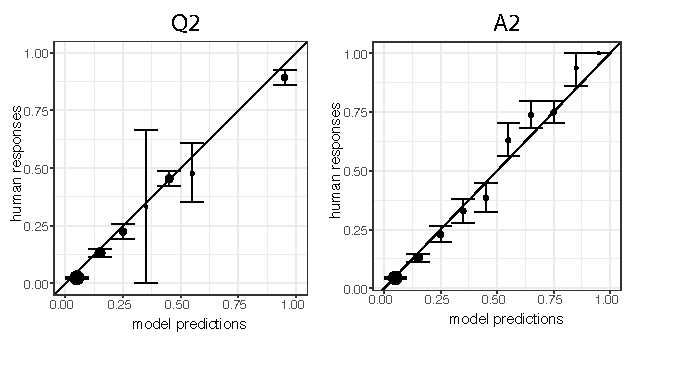
\includegraphics[scale = .8]{Exp3/predictives.pdf}
\end{center}
\caption{Posterior predictives for each model, binned to intervals of length 1/10.}
%\vspace{-1cm}
\label{fig:exp3predictives}
\end{figure}


%\begin{figure*}[tbh!]
%\begin{center}
%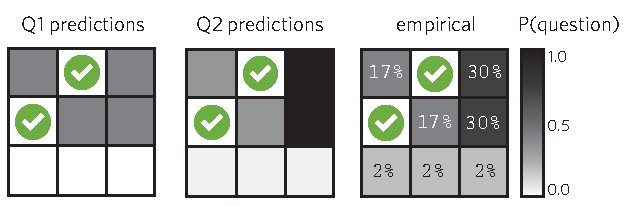
\includegraphics[scale = .7]{Exp3/spatialQualitativeQuestioner.pdf}
%\end{center}
%\caption{Posterior predictives for each model, which indicate good overall fit (excluding $A_0$ and $Q_0$). Blue dots on $Q$ plots indicate overlapping condition.}
%%\vspace{-1cm}
%\label{fig:exp1predictives}
%\end{figure*}

% \subsection{Discussion}
%To generalize to dialogues lasting longer than a single exchange, we must specify the way in which the contributions of questioner and answerer affect the \emph{context} in which later utterances operate, and the longer-term planning needed for agents to reason effectively about such interactions.

%\cite<e.g>{khani2018planning,young2013pomdp,gao2019neural}

\section{General discussion}
\label{sec:gd}

%\todo[inline]{Might split this into subsections?}
% \subsection{Summary of what we did}

Asking questions is one of our most efficient and reliable means of learning about the world. 
Yet we do not often pose these questions to an impartial oracle; we ask other agents, in dialogue. In this paper, we jointly consider the decision problems faced by socially aware questioner and answerer agents. 
Questioners must plan over the possible answers they are likely to receive from their partner and seek to maximize the future reduction in their own uncertainty. 
Answerers, in turn, seek to informatively and relevantly address the underlying goals most likely to have motivated the question. 

%\todo[inline]{Refactor next paragraph to separate out stuff that's included in the model from external stuff}
We provided several lines of evidence supporting this theory---formalized in our $A_2$ and $Q_2$ models---over asocial questioners and answerers. 
In a series of answerer simulations, we showed that only $A_2$ could qualitatively account for classic answerer-sensitivity effects from \citeA{Clark79_IndirectSpeechActs}: answers depend critically upon the question utterance, the context in which a question is asked, and the relationship between the questioner's underlying goal and their question. 
We then found strong qualitative and quantitative evidence for both $A_2$ and $Q_2$ from three dialogue experiments in our \emph{Hidden Goal} paradigm, which further demonstrated the extensibility of our core framework. %as well as strong quantitative evidence from a rigorous model comparison on trial-by-trial data. By  in this experiment, we also observed systematic use of indirect questions, as predicted by $Q_1$ and $Q_2$. However, only $Q_2$, who relies on higher-order pragmatic reasoning about what goals an answerer would infer from their question utterance, could account for the critical overlapping condition. 
%Finally, enriching the semantics of ``Where is \emph{the}\dots?'' questions to use more realistic saliency priors both eliminated a potential confound and also significantly improved our quantitative fit. %, questioners relied on higher-order pragmatic reasoning about what inferences an answerer would make about their own underlying goals when deciding what question to ask, but a Bayesian model comparison showed that the simpler explicit model is sufficient to explain the vast majority of our data.

%In the case of our Experiment 1 hierarchy, there exists a simple, heuristic strategy that produces the same pattern of responses as our model without requiring any social inference. Suppose questioners saw their goal on a given trial and ruled out labels that do not apply (e.g. a `cat' is neither a `dalmatian' nor a `dog'), then picked the most specific of the remaining labels (`pet' picks out a smaller set of objects than `animal'). Whether through use of this heuristic strategy or pragmatic inference (as our model suggests), questioners strongly converged on a single mapping from goals to question utterances. 

% Note that this behavior also could not be explained by the heuristic strategy raised in the earlier experiments: if questioners just ruled out labels that did not apply (e.g. ``lion''), they would have no mechanism for deciding between the two equally-good parent labels (``pet'' and ``cat'') to pick out their goal. 

A central theoretical advance of the proposed framework is the synthesis of current (OED) approaches to optimal question asking, in active learning, with the generic social reasoning mechanisms proposed by the Rational Speech Act approach to language use. 
In addition to embedding the former approaches into a social context, this work moves RSA models beyond the production or interpretation of single utterances (in context) to consider the dynamics of simple dialogs where both listening and speaking---linguistic input and output---must be integrated within the same agent. 
In the remainder of the discussion we address several broader issues raised by our framework and note a number of avenues for future work.

\subsection{What is the meaning of a question?}

While our framework draws extensively from previous theoretical accounts of question and answer semantics, the division of labor between semantics and pragmatics in our proposed model leads to a subtly different perspective on the meaning of a question. 
These differences stem from two psychologically meaningful distinctions at the core of our model.
The first disentangles the literal meaning of a question from any particular set of possible answers and instead associates it with a specific goal that it raises or signals for an answerer.
The second disentangles the space of possible latent goals in the questioner's mind from the one associated with the interrogative signal they choose to provide.
Together, these distinctions allow us to \emph{derive} context-sensitivity at the pragmatic level via social reasoning that grounds out in context-independent meanings.

This idea differs somewhat from the context-sensitive literal meanings suggested by \citeA{VanRooy03_QuestioningDecisionProblems}.
As previously described, Van Rooy argued that the meaning of a question ought to be underspecified and resolved only through the contextual parameter of the questioner's decision problem.
Once we explicitly address the issue of how the answerer actually \emph{infers} this decision problem from hearing the question (and from other context), it becomes unnecessary to additionally posit underspecified literal question meaning.\footnote{RSA models have handled vague or underspecified literal meanings by introducing a free variable into the meaning that is determined by the speaker and inferred by the pragmatic listener \cite<e.g>{LassiterGoodman15_AdjectivalVagueness,TesslerGoodman16_Generics}\ndg{cite bergen levy goodman}. An implementation of van Rooy's proposal would require the free variable in the literal meaning to be the derived from the questioner's private goal itself. It is unclear whether this mechanism would lead to appropriate interactions between context and question interpretation.}
Because we take a goal to be the same type of object as a classic partition-based question meaning \cite{GroenendijkStokhof84_SemanticsOfQuestions}, we can implement its meaning in a literal answerer who identifies the goal directly from the question.

In this way, the meaning of a question in our framework resonates with dynamic accounts of question meaning \cite<e.g>{Groenendijk99_LogicOfInterrogation}, as well as recent proposals for an inquisitive semantics \cite{ciardelli2018inquisitive}, where the formal content of a question is simply the ``issue'' it raises into the context.
Our proposal that the meaning of an interrogative sentence shifts the hearer's beliefs about the questioner's goals can be seen as a probabilistic analogue to the notion of \emph{inquisitive content} as implemented in formal logic.
%Similarly, our proposal that  is  to o from standard informational content. 
% roughly corresponding to our distinction between the  while declarative sentences shift beliefs about the state of the world.
In both cases, defining literal question semantics directly in terms of their inquisitive content rather than possible answers imposes a crucial \emph{modularity} at the semantic level of the model. 
This modularity frees higher-level pragmatic considerations to handle the problem of how questioners actually think their partner will generate answers given a question, which may or may not correspond to the literal resolution conditions.

The connection to inquisitive semantics is an intriguing area for further exploration. % and we see the broader correspondence between probabilistic and logic-based notions of inquisitive content .
For example, a fundamental insight of inquisitive semantics is that declarative sentences sometimes \emph{also} have inquisitive content.
While we have made the simplifying assumption that declarative utterances are purely informative, the RSA framework could also support this ``hybrid'' notion.
For example, previous RSA models have explained the use of non-literal language like hyperbole, irony, and metaphor in declarative sentences by the same mechanism we invoked here: providing information about the speaker's goal \cite{KaoEtAl2014-Cogsci,KaoGoodman15_IronyCogSci,KaoWuBergenGoodman14_NonliteralNumberWords}.
A subtler difference, however, lies in the correspondence between the projection function we have used to define goals and the ``issue'' formalism in inquisitive semantics, which is not as strict. 
Thus, the class of functions used to represent a goal in our framework may need to be expanded to properly handle embedded questions, entailment, and disjunction \cite{ciardelli2018inquisitive}.


%\subsection{Limitations of the model}

%We emphasize that all our models are situated firmly at the computational level \cite{Marr10_Vision} -- these models formalize hypotheses about the problem being solved by questioners and answerers in dialogue, and they make quantitative predictions about expected behavior under different assumptions. However, we do not propose that people are actively running a recursive probability calculation online every time they ask a question; further work is needed at the algorithmic and mechanistic levels to understand exactly what cognitive and neural processes give rise to the computations we predict, especially when it comes to integrating information across discourse contexts. 

%While these results provide strong evidence for our claim that question-asking and answering is grounded in sophisticated social reasoning, it is worth more closely examining some choices we made in formulating our Rational Speech Act model. For example, as in previous studies using RSA, we assume that the recursive reasoning process giving rise to pragmatic interpretations grounds out in a base case of literal semantics. We only consider two levels of recursion above this base case, but we could in principle consider a fixed-point at infinity \cite{Franke13_GameTheoryPragmatics}. Alternatively, social reasoning could be grounded not in iterated reasoning but in a joint project or shared intention established by other means \cite{Clark96_UsingLanguage, TomaselloCarpenter___Moll05_IntentionsCulturalCognition}. While we suspect the question-answer domain is not particularly informative for distinguishing between these formulations, we note that additional levels of reasoning tend not to qualitatively change RSA predictions and that our model contains elements of the latter proposal in its assumption that questioners and answerers share priors, sets of alternatives, and semantic meanings in common ground \cite<see>[for further discussion]{LassiterGoodman15_AdjectivalVagueness} 

 
\subsection{The correspondence between questions and goals}

A straightforward consequence of defining the meaning of a question to be the same kind of object as a goal, is that our $Q_2$ model predicts that people will ask the question most directly corresponding to their private goal if it accessible and easy to produce.
After all, it would be the clearest signal.
So why would a questioner ever ask a question that didn't directly correspond to their underlying goal? 
Our dissociation of question meanings and latent goals raises the interesting possibility that the set of questions that is easy to verbally express is effectively a \emph{subset} of the possible latent goals one might have: there may not exist a question utterance literally encoding every underlying goal an agent may need to address, thus the need for pragmatics.

More specifically, we were motivated by real-world cases where the interrogative sentence with a meaning more closely corresponding to the underlying goal would be longer or more confusing to produce. 
For instance, when trying to meet up in a city, people regularly get away with asking the bare question ``Where are you?'' when they could directly signal the relevant coarse-graining, e.g. ``At the intersection of which two streets are you currently located, and which direction are you heading?'' \cite{Potts12_CardsDialogueCorpus}.
While we leave a careful formal account of ``Where are you?'' in our framework for future work, it seems natural for the literal meaning to be the finest-grained goal of locating the hearer's exact point in space, such that higher levels of pragmatic recursion coarsen it to the appropriate level.
Pragmatic questioners will prefer the less costly utterance if they can expect the answerer to recover the intended coarser goal.
Issues of cost may enter \emph{answers} to ``Where are you?'' as well, since giving a precise GPS coordinate is presumably costlier than more coarse-grained and easily retrievable spatial referring expressions.

Empirically, it was challenging to naturally capture such cost differences for our controlled experiments; instead, we imposed this cost artificially by disallowing the most direct questions for some scenarios. 
Under this constraint, we were able to test the model's preferences among alternative questions.
%We would observe similar model predictions if we had included these disallowed questions in the model's question set $\mathcal{Q}$ but given them higher production costs.
This does not invalidate our model comparison, but it does leave open for future work the empirical challenge of designing a lab task that can naturally modulate the cost of the direct question. 
Other empirical paradigms for question-asking also tend to impose strict constraints on allowable questions for similar reasons. 
In games like Battleship or 20 Questions, the truly optimal questions would be ``Where are all of your ships?'' or ``Which object are you thinking of?''

%\todo[inline]{Revamp this para... Say our work may shed new light on why not generating perfectly optimal questions may not be a problem in social interaction; if they're used to relying on the answerer to make inferences, they may go for a cognitively cheaper question that still effectively signals the goal. so people may still be cognitively limited in their ability to generate questions but these less informative questions may be `resource-rational' given social expectations of cooperativity (see our ToM paper?)}
These considerations may also shed new theoretical light on recent results by \citeA{rothe2018people} finding that in games like Battleship, people often fail to ask maximally informative natural language questions (although they \emph{can} accurately rank the informativity of pre-generated questions). 
By embedding questioning in a social, communicative context \cite<see also>{ShaftoGoodmanFrank12_LearningFromOthers, ShaftoGoodmanGriffiths14_Pedagogical}, our framework suggests that this behavior may in fact be resource-rational under the conditions where most questioning takes place \cite{GriffithsLiederGoodman15_LevelsOfAnalysis}.
If the maximally informative questions are longer and more syntactically or conceptually complex (e.g. ``At what location is the top left part of the purple ship?''), they may also be more cognitively demanding to generate.
When assuming a cooperative pragmatic answerer, however, a less costly question may be just as effective for signaling the goal and getting a helpful answer.

\subsection{Computational challenges}

How do our assumptions scale up to less constrained interactions? 
We suspect that the simple, discrete sets of goals used in our models above may need to be generalized to continuous spaces and broader mixtures of discourse topics \cite{BleiNgJordan03_LDA, GriffithsSteyversTenenbaum07_Topics}. 
The computational challenges associated with such complex goal spaces may contribute to the difficulties young children face in answering broad, sentence-focus questions like ``what's happening?'' \cite{SalomoLievenTomasello13_ChildrenAnsweringQuestions}. 
%Similarly, to generalize beyond the tightly controlled sets of alternative questions and answers used in our models above, we may need to consider empirical frequencies or simple deletions and edits from the given question to automatically generate sets of alternatives \cite<e.g.>{GibsonBergenPiantadosi13_RationalIntegrationNoisy}. 

As a broader point, our framework offers a rational analysis of the social inferences involved in asking and answering questions, which only adds to the many important algorithmic questions already raised by rational model of inquiry \citeA{coenen2018asking}.
For instance, we could use without modification the sophisticated and open-ended grammar of questions developed by \citeA{rothe2017question} as the prior for the question set $\mathcal{Q}$ in our pragmatic framework, but this would turn the literal questioner agent $Q_1$ into an infinite distribution, leading to very difficult inference at higher levels of recursion.
Similarly, taking an analytic expectation over all possible worlds quickly becomes intractable as the size of the world space $\mathcal{W}$ grows.
We used exact enumeration for all of our results for theoretical precision, but it is clear that an algorithmic account must address how these computations can be effectively approximated, perhaps via Monte Carlo integration of approximation by neural networks.

%\todo[inline]{finally, note that even though we offered a rational analysis of what is required to solve this problem through Bayesian reasoning, aspects of the computation such as the goal prediction problem may be approximated by a feed-forward neural network}

%\todo[inline]{Maybe here is a good place to address R2's concern about `hand-coding' meanings, and not being falsifiable? e.g. this raises concerns that our model could fit \emph{any} question-answer data by choosing the appropriate set of priors. Indeed, we regard all of these choices as scientific hypotheses, not free parameters. For the experiments presented in the rest of this paper, we test these hypotheses or fix them via our experiment design. The choices in the computational experiments above were simply intended to be reasonable enough to illustrate how our model framework accommodates various results from the literature on question-answer pragmatics.}

\subsection{Applications to other question phenomena}

While the applications throughout this paper have primarily focused on canonical \emph{epistemic} questions in a cooperative context, our framework also provides a tool set for formalizing pragmatic accounts of other question phenomena. 
We briefly highlight four potential applications: rhetorical questions, pedagogical questions, politeness, and uncooperative interrogation.

First, rhetorical questions are characterized by being either completely obvious or completely unanswerable (\emph{What's going to happen to these kids when they grow up?}).
A pragmatic answerer hearing such a question in our framework would reason that a questioner is unlikely to have chosen it with the epistemic goal of getting information and instead must have another goal in mind such as signaling common ground or expressing affect \cite{KaoWuBergenGoodman14_NonliteralNumberWords}. 
In this way, one could derive the assertive force of rhetorical questions from pragmatic principles \cite<see>{Rohde06_rhetorical}.

Second, consider how we could account for pedagogical questions asked by parents or educators \cite{MaradlouGinzburg14_SemDial, Gall70_QuestionsInTeaching}. 
A math instructor asking a question like ``what is $2+2$?'' already knows the answer, so what utility could there be in asking? 
Instead of trying to reduce their own epistemic uncertainty over the result of the math problem, perhaps the teacher is instead trying to reduce their uncertainty over the child's knowledge state. 
If we introduced such uncertainty about the answerer's background knowledge in our model and gave the questioner the goal of determining this background knowledge, it would be rational to ask targeted questions that would expose the answerer's knowledge. 

Third, we return to indirect speech acts like ``Do you know where I can find a restroom?'' 
These indirect forms of questions are often analyzed as being motivated by \emph{politeness}, since they pinpoint likely obstacles to answering \cite{FrancikClark85_RequestsOvercomeObstacles} and give answerers an easy way to opt out \cite{brown1987politeness}.
The same politeness considerations may influence answerer behavior as well. 
For instance, when people do give literal answers they may use more words than necessary to avoid seeming curt or unhelpful \cite<see also>{chaudhry2019thanking}. 
%are often something like `yes, I do' or `no, but good luck!' One way to think about this is that the questioner has some uncertainty over the answerer's relative balance between utterance cost and helpfulness, and questioners will jointly infer this. 
Such politeness considerations have been formally incorporated into RSA models as a kind of goal that takes into account social and presentational utilities \cite{yoon2016talking}, which could be straightforwardly incorporated into a questioner model.

Finally, although we have assumed basic prosociality and transparency in our agents, some of the most intriguing question-answering scenarios flout this expectation. 
In politics or court of law, for instance, it is sometimes in the answerer's best interest to be minimally informative while still appearing to address the literal semantics of the question.
Indeed, a key legal question is whether such ``bad-faith'' literal answers can constitute perjury \cite{SolanTiersma05_SpeakingOfCrime}. 
In other cases, questioners may want to conceal or deceive the answerer about their true goals while still obtaining information (e.g. when gathering information to buy a gift.)
To understand behavior in these cases it may be necessary to adjust the utility to \emph{minimize} the reduction in uncertainty, or to assume the answerer is further down the recursion hierarchy than we found to be empirically the case in our experiments.
% , or to identify when an answerer is being uncooperative, 


\subsection{Conclusion}
Humans are experts at inferring the intentions of other agents from their actions \cite{TomaselloCarpenter___Moll05_IntentionsCulturalCognition, BakerSaxeTenenbaum09_ActionUnderstandingInversePlanning}. Given simple motion cues, for example, we are able to reliably discern high-level goals such as chasing, fighting, courting, or playing \cite{BarrettToddMillerBlythe05_IntentionFromMotionCues, HeiderSimmel44_Animacy}. A long tradition in psycholinguistics has shown that this expertise extends to speech acts.  Behind every question lies a goal or intention. This could be an intention to obtain an explicit piece of information (``Where can I get a newspaper?''), signal some common ground (``Did you see the game last night?''), test the answerer's knowledge (``If I add these numbers together, what do I get?''), politely request the audience to take some action (``Could you pass the salt?''), or just to make open-ended small talk (``How was your weekend?''). These wildly different intentions seem to warrant different kinds of answers. %, even if the explicit question is expressed using the same words
By formalizing the recursive utilities of questioner and answerer agents and the computational principles by which agents infer each other's intentions from verbal behavior, our framework provides a foundation for re-situating question asking and answering in its social context.

\section{\bf Acknowledgments}
\small
\noindent We thank Leon Bergen, Judith Degen, Andreas Stuhlm\"uller, Arianna Yuan, MH Tessler, Dan Lassiter, and Judith Fan for thoughtful conversations and comments. This work was supported by ONR grants N00014-13-1-0788 and N00014-13-10341. RXDH was supported by the Stanford Graduate Fellowship and the National Science Foundation Graduate Research Fellowship under Grant No. DGE-114747.

\bibliography{qa}
\bibliographystyle{apacite}


\begin{table*}[t!]
\centering
\begin{tabular}{ p{1.5cm} | r | r | r | r |||||| r | r | r | r |}
& \multicolumn{4}{c||||||}{Questioners} & \multicolumn{4}{c}{Answerers} \\
&             animal &     place &     plant &  artifact &            animal &     place &     plant &  artifact \\
\hline
animal &   1.00 &  0.91 & 0.94 & 0.94 & 1.00 & 0.78 & 0.92 &  0.97 \\
\hline
place &    0.91 &  1.00 & 0.96 & 0.95 & 0.78 & 1.00 &  0.78 & 0.78 \\
\hline
plant &    0.94 & 0.96 & 1.00 & 0.97 & 0.92  & 0.78 &  1.00 & 0.91\\
\hline
artifact & 0.94 & 0.95 & 0.97 & 1.00 & 0.97 & 0.78 &  0.91 & 1.00\\
\end{tabular}
\\[1.5pt]
\caption{Appendix: Inter-domain correlations on corresponding response rates} 
\label{table:experiment4correlations}
\end{table*}

%\section{Appendix}
%
%\subsection{Groenendijk and Stokhof (1984)}
%%\begin{figure*}[t!]
%%\begin{center}
%%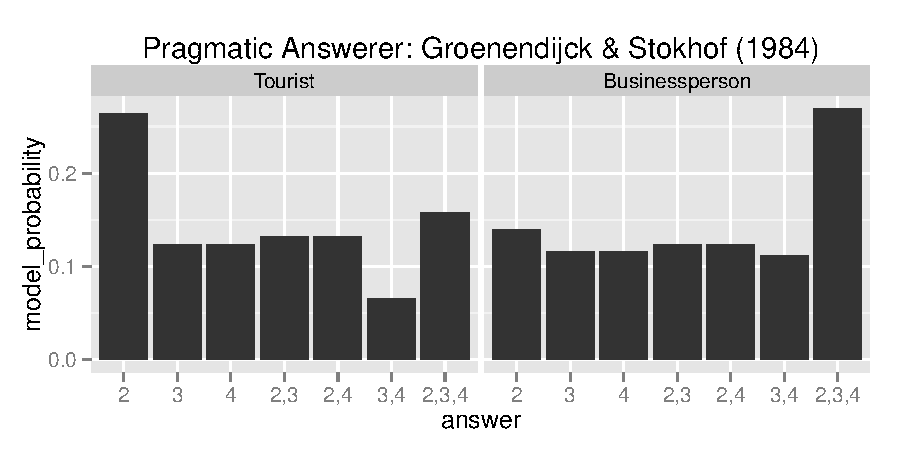
\includegraphics[scale = 1]{groenendijckPlot.pdf}
%%\end{center}
%%\vspace{-.25cm}
%%\caption{Results for our computational experiments implementing the Groenendijck \& Stokhof (1984) \emph{mention-some} problem.}
%%\label{fig:cafeExperimentResults}
%%\end{figure*}
%
%%Here, we consider the classic puzzle of \emph{mention-some} and \emph{mention-all} readings of wh-questions  \cite{GroenendijkStokhof84_SemanticsOfQuestions}. 
%Some \emph{wh-}questions, like ``Who is coming to dinner tonight?'' are intended to elicit an \emph{exhaustive} list of the entities that are answers. For ostensibly similar questions, like ``Where can I find a bathroom in this building?'', a mention of a single location would be sufficient. Many recent theoretical explanations of this phenomenon in the linguistics literature appeal to questioner goals \cite<e.g.>{SchulzVanRooij06_ExhaustiveInterpretation, Ginzburg95_ResolvingQuestions}, which is easily formalized in our model as a context-prior. 
%
%We focus on a question like ``Where do they sell Italian newspapers in Amsterdam?'' that can intuitively be ambiguous between these meanings depending on who is asking: if it is a tourist, they probably just want to know the nearest place, but if it is a businessperson trying to build a newspaper distribution network, they likely want the whole list \cite<see>{GroenendijkStokhof84_SemanticsOfQuestions}. The puzzle is  one of disambiguation\footnote{Our modeling framework is compatible with another account where the `mention-some' reading is derived from the exhaustive reading via implicature \cite<e.g.>[Chapter 6]{George11_Dissertation}, but this debate lies outside the scope of this paper}: how can the same question take on different meaning in different contexts? According to our account, this happens via an inference about the questioner's underlying goal. This explanation relies on the same mechanism as the previous section, but shows how the model can operate over more complex world states and arbitrarily large spaces of possible answers.
%
%Our world space $\mathcal{W}$ consists of all possible assignments of properties to a set of four cafes in town. Each cafe has two properties: its distance from the speaker and whether or not it sells Italian newspapers. There are two possible goals (or QUDs) $g \in \mathcal{G}$: $g_{n}$, learning the identity of the \emph{lowest-cost} cafe selling a newspaper, and $g_{a}$, learning the identity of \emph{all} cafes selling a newspaper. Both of these are represented by projections on world states, mapping a list of cafes to the single cafe selling newspapers with the lowest distance -- assuming that additional distance incurs additional cost -- or to the sublist that sell newspapers, respectively. \ndg{why talk about cost, rather than just saying closest?} The space of answers $\mathcal{A}$ is the infinite set containing all conjunctions of locations. \ndg{is that infinite? up to redundancy it's large but finite?} Again, our question space $\mathcal{Q}$ consists of a single question: ``Where can one buy an Italian newspaper?'' \ndg{what literal meaning do we assign to this question?}
%
%For the prior $P(a)$ over answer utterances, we use a geometric distribution, which is common over spaces where probabilities should naturally scale with some count. Let $\ell(a)$ be the number of locations named in the answer (e.g. $\ell(\textrm{`none'})~=~0, \ell(\textrm{`cafe 1'})~=~1$, etc). Then the probability of an answer $a$ is given by:
%
%$$P(a) \propto (1 - p)^{\ell(a)}p$$
%In our computational experiment, we fix $p = 0.8$. 
%This simple distribution has two advantageous properties: 
%\begin{enumerate}[(1)]
%\item the probability mass assigned to a given utterance length -- operationalized as number of conjunctions -- by the geometric distribution is spread evenly across different answers of that length.
%\item we naturally assign longer answers successively lower probability, reflecting their higher cost of utterance. \end{enumerate}
%
%\ndg{i think we can a say a lot less about this prior: just that we assume the cost of an answer is proportional to it's length, hence the prior is proportional to $\exp(length)$...}
%
%
%We model the non-verbal context as affecting the questioner's goal prior $P(g)$: if they are a tourist on the street then there's a high chance that they are interested in buying a single newspaper, and hence knowing the identity of the closest shop that sells Italian newspapers ($P(g_n | c) = 0.99$); if they're a businessperson in a boardroom, then there's a high chance that they are interested in the exhaustive list of all of the Italian newspaper locations ($P(g_a | c) = 0.99$).
%
%%\footnote{Note that this formulation of the problem differs slightly from the one given by \citeA{GroenendijkStokhof84_SemanticsOfQuestions}, although they easily map onto one another. In the original formulation, the \emph{answer} is fixed and the \emph{meaning} of the answer must be inferred to either be mention-some or mention-all. In our formulation, the meaning of each answer is unique and fixed, but the answerer must choose among a set of different possible answers. The same inferential machinery that our questioner uses to reason about which answer utterance the answerer will give could also be used to reason about which \emph{meaning} the answerer intends by their fixed utterance. The only difference is that the questioner would have uncertainty over a set of possible meanings instead of uncertainty over a set of possible answer utterances. We chose the latter because it more closely resembles the other scenarios we are modeling.}
%
%It is unclear where these goals and goal priors may come from in real-world situations: it is likely tied to background knowledge about tourists, newspapers, and the business world, as well as past experience in social situations. While these deeper explanations lie outside the scope of our model, we still have explanatory power in showing how goals interact with other terms, and how the prior differ across scenarios. 
%
% \begin{figure*}[t!]

%\ndg{i didn't re-read this appendix... there seem to be old comments of mine left?}

%\begin{figure*}[t!]
%\begin{center}
%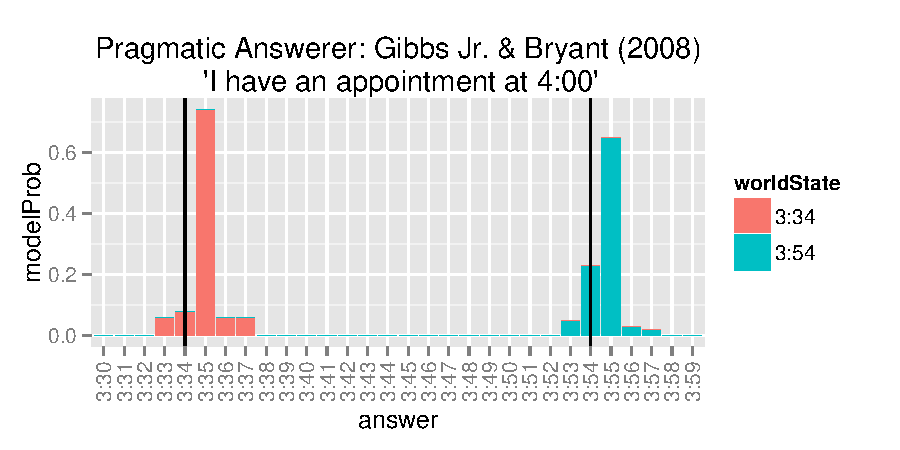
\includegraphics[scale = 1]{timeExpResults.pdf}
%\end{center}
%\vspace{-.25cm}
%\caption{Results for our computational experiments replicating Gibbs Jr. and Bryant (2008). Vertical lines represent the true world state.}
%\label{fig:timeExperimentResults}
%\end{figure*}
%
%\subsubsection{Results}
%
%For concreteness, we set the true world to be the following :
%
%\begin{lstlisting}
%world = {`cafe1' : [3, false],
%         `cafe2' : [1, true],
%         `cafe3' : [3, true],
%         `cafe4' : [3, true]}
%\end{lstlisting}
%meaning that `cafe1' is three blocks away from the speaker and does \emph{not} sell Italian newspapers, `cafe2' is one block away and \emph{does} sell Italian newspapers, and so on. We used \emph{likely-first enumeration} over the answerer model, stopping after 1000 executions of the infinite answer space (longer answers were assigned vanishingly small probability). We find that the highest probability response given the ``tourist'' context is the single location ``cafe2.'' When worlds consistent with this utterance (i.e. where cafe2 truly sells an Italian newspaper) have been projected to the closest location, the actual closest location has high probability, thus informatively fulfilling the contextually more likely goal $g_n$. Note that longer responses are unlikely for two converging reasons: they're less likely under the geometric answer prior and also may mislead the questioner into thinking another location is the closest. 
%
%Given the ``businessperson'' context, however, the highest probability response is the conjunction ``cafe2 and cafe3 and cafe4.'' This is the exhaustive answer, informatively fulfilling the contextually more likely goal $g_a$ of knowing the location of all cafes selling Italian newspapers. Shorter answers are less likely; they are consistent with more possible worlds in the projected space, hence the projection of the true world has lower probability. 
%
%\ndg{it occurs to me that if you ignored the question and just took the goal to be the qud you'd get the same results. maybe we'd like to have a more likely a priori goal that get's dis-preferred after hearing the question? for instance the identity goal could be a priori more likely, but then becomes less plausible after hearing the question about italian papers?}
%
%%The literal and explicit answerers, as in the Clark scenario, do not have the means of making inferences about the questioner's underlying goals. Thus, both models incorrectly predicted that the context would not affect the preferred response. The literal answerer predicted that all combinations of cafes 2, 3, and 4 would be given in proportion to their prior likelihood (with no special preference given to the closest one). The explicit answerer predicted that the exhaustive answer would be preferred in all contexts (as this is literal semantics we encoded for the question). 
%Crucially, the only difference between our model of this scenario and the Clark scenario is the richer representations of multi-dimensional world states, and the larger (unbounded) space of answers. The model itself was unchanged; we only enriched the content of its inputs. The mechanism by which goals were inferred in both cases, however, was the same: a direct function of verbal or non-verbal context. Next, we turn to a case where the world state itself provides a clue to the questioner's goal.
%%%%%
%
%
%\subsection{Gibbs Jr. \& Bryant (2008): Experiment 3}
%
%It has been shown in previous work that speakers typically round their answers to the nearest 5 minute interval when asked `Do you have the time?'', even when they're wearing a digital watch \cite{DerHenstCarlesSperber02_RelevanceTellingTime}.  \citeA{GibbsBryant08_OptimalRelevance} replicated this result, and then performed a follow-up study on analog-watch wearers where they preceded their question by the context ``I have a meeting at 4:00.'' 
%
%They found that the tendency to round times decreased as a function of the time remaining until the stated deadline: the group asked 30-16 minutes before the stated appointment rounded their responses 79\% of the time, while the group asked 14 minutes or closer to the appointment rounded significantly less (62\%). They explained this result by appealing to the questioner's goals: while an approximate time is sufficiently informative with respect to most goals, such as knowing how much time is left before heading to an appointment, a questioner who is running late may need to gauge how quickly they should move, whether they should call and warn about being late, or make other such decisions, in which case a precise time is highly relevant. 
%\begin{table*}[t]
%\centering
%\begin{tabular}{ p{2cm} | r |||||| r }
%&  \% round (Empirical) &  \% round (Model) \\
%\hline
%Early group &  0.79 & 0.77 \\
%\hline
%Late group     &0.62  & 0.60 \\
%\end{tabular}
%\\[1.5pt]
%\caption{Comparison of our model predictions with data from Gibbs Jr. and Bryan (2008). Shows the proportion of rounding in response to ``I have an appointment at 4:00. Do you have the time?'' for two groups: an ``early group'' where the appointment was in 30-15 minutes and a ``late group'' where the appointment was in less than 15 minutes.} 
%\label{table:gibbsJrExp3}
%\end{table*}
%
%To set up this scenario in our model, we take the world space to be the set of possible times, which we limit to a half hour interval (as in the experiment): $\mathcal{W}~=~\{\textrm{3:30}, \textrm{3:31}, \dots, \textrm{3:59}\}$. Unlike in the previous two case studies, where there were only two contrasting goals and two contexts that make each goal more or less likely, we now use a larger, parametrized goal space and a single context stating the time of the appointment that is held fixed across different conditions of the experiment. 
%
%This goal space $\mathcal{G}$ includes the trivial projection $g_0(w) = w$, corresponding to the context-independent goal of learning the true time, in addition to a set of goals parameterized by a threshold time $\tau$, representing the point at which the agent believes they are running late to their appointment (likely based on expectations about travel time, social norms concerning lateness, and other exogenous factors). If the agent has goal $g_\tau$ for a given $\tau$, then for times $t < \tau,$ the agent only cares about the approximate time, rounded to the nearest 5 minute increment, in order to know roughly how much time they have before leaving. For times $t > \tau$, the agent cares about the exact time in order to make the kind of decisions described above. Formally,
%
%\DeclarePairedDelimiter{\floor}{\lfloor}{\rfloor}
%
%$$g_\tau(w) = \left\{
%\begin{array}{rcl}
%w & & w \ge \tau\\
%5\floor{\frac{w}{5} + \frac{1}{2}} & & w < \tau;  \\
%\end{array}
%\right.
%$$
%where $\floor{w}$ returns the \emph{floor} of an integer and all operations are assumed to act on the minutes component of a time $w$. For example, the goal $g_{3:50}$ with the threshold set at $\tau = $3:50 corresponds to a projection function that rounds input worlds earlier than 3:50 and does not round worlds later than 3:50. This would be the case if the agent knew they would need to leave around 3:50 in order to make it to an appointment on time. 
%
%The goal prior $P(g_\tau)$ assigns probability $p=0.25$ to the context-independent goal $g_0$ of wanting to know the exact time. The remaining probability mass is divided across different threshold goals ($\tau \in \{$ 3:31, 3:32, \dots, 3:59 $\}$) according to the following rule: the likelihood of each goal $g_\tau$ is inversely proportional to the distance (in minutes) between the threshold $\tau$ and the given appointment time $c$, reflecting the intuition that the questioner will be more likely to be running late, and therefore in need of the exact time, as it approaches the appointment time:
%
%$$P(g_0) = 0.25$$
%$$P(g_\tau; c) = \frac{0.75}{\sum_{i=1}^{29}i}(30 - |\tau - c|)$$
%
%The set of answers is the set of times that could be given (e.g. 3:30, 3:31, \dots, 4:00), with multiples of 5 preferred:
%$$P(t) = \left\{
%\begin{array}{lcl}
%0.125 & & t \equiv 0 \mod 5 \\
%0.01 & & \textrm{otherwise} \\
%\end{array}
%\right.
%$$ As \citeA{GibbsBryant08_OptimalRelevance} point out, their participants all wore analog watches, hence precise answers have higher cost. In fact, an earlier study in the same paper showed that in the absence of any context, participants wearing analog watches responded with rounded answers 90\% of the time, so this prior is realistic. 
%
%For our answers, we use exact number semantics: the response ``3:35'' evaluates to true in worlds where the time is in fact 3:35, and false otherwise. While we suppressed \emph{a priori} false answers for convenience in other case studies (they would be naturally be assigned vanishingly small probability anyway), note that we cannot do so here: answerers must be allowed to make \emph{a priori} false utterances that get reinterpreted by the listener to be true under the QUD \cite<see>{KaoWuBergenGoodman14_NonliteralNumberWords}. 
%
%%\todo[inline]{return to this in the discussion}
%
% \subsubsection{Results}
% 
%To compare our model's performance against the `early group' and `late group' conditions in \citeA{GibbsBryant08_OptimalRelevance}, we ran two simulations. In both, the context is ``I have an appointment at 4:00.'' In the first, the true world state is between 3:30 and 3:45 (the `early' condition); in the second, the true world state is between 3:45 and 3:59 (the `late' condition). In each condition, we ran our pragmatic answerer model for all true worlds in the appropriate range of times, and report the average probability of responding with a rounded answer. Our results are compared against empirical data from Gibbs Jr. and Bryant \citeyear{GibbsBryant08_OptimalRelevance} in Table \ref{table:gibbsJrExp3}. 
%
%To more closely analyze what is driving our model's performance in these two conditions, we examine the answer behavior for two specific world states: one from the `early group' (3:34) and one from the `late group' (3:54). Answer probabilities for these two conditions are shown in Figure \ref{fig:timeExperimentResults}. We found that our pragmatic answerer model rounds the 3:34 to 3:35 in the `early' condition with probability $p = 0.74$, but rounds 3:54 to 3:55 with lower probability $p = 0.65$ in the `late' condition. 
%
%The goal prior is the key component of the model governing this difference. Note that that (1) \emph{all} states in the pre-image of the rounding projection from the true time $t_0$ are assigned lower probability than the rounded time $g_\tau(t_0)$, due to the influence of goals $g_\tau$ with thresholds $\tau > t_0$ and (2) the true time $t_0$ is assigned relatively higher probability than the other non-rounded times, due to the influence of the pure goal $g_0$ and goals $g_\tau$ with thresholds $\tau < t_0$. This dynamic, paired with the upward-skewed prior on goal priors discussed above, causes the `late' condition to assign a much higher relative probability to the true time, than the `early' condition. The pragmatic answerer thus accurately captures the empirical results both qualitatively and quantitatively. 

%Our literal and explicit answerer models fail to capture these contextual differences, as they do not reason about the space of underlying goals (which justify rounding) and always give the exact time. The literal answerer always gives the exact time because it is the only property of the world, which they are attempting to be informative about without regard to the question. The explicit answerer always gives the exact time because it uses the explicit question meaning, which simply asks for the time.

%\todo[inline]{rdh: Actually, in the experiment the question was ``Do you have the time?'' to which the literal and explicit answers would be ``yes'' or ``no'', right? We don't allow these responses in our model because they're not what we're interested in (i.e. \emph{no one} responded this way), but they are the kinds of answers our literal and explicit answerers would give}

\end{document}  
